%%Below is the guy I stole this template from, because it is great
%%%%%%%%%%%%%%%%%%%%%%%%%%%%%% -*- Mode: Latex -*- %%%%%%%%%%%%%%%%%%%%%%%%%%%%
%% uhtest-body.tex -- 
%% Author          : Robert Brewer
%% Created On      : Fri Oct  2 16:30:37 1998
%%%%%%%%%%%%%%%%%%%%%%%%%%%%%%%%%%%%%%%%%%%%%%%%%%%%%%%%%%%%%%%%%%%%%%%%%%%%%%%
%%   Copyright (C) 1998 Robert Brewer
%%%%%%%%%%%%%%%%%%%%%%%%%%%%%%%%%%%%%%%%%%%%%%%%%%%%%%%%%%%%%%%%%%%%%%%%%%%%%%%
%% 

%% And then I'll add stuff for myself as well
%% uhtest-body.tex -- 
%% Author          : Benjamin Rotter
%% Created On      : Fri January 24th 2017
%% Last Modified By: Benjamin Rotter
%%%%%%%%%%%%%%%%%%%%%%%%%%%%%%%%%%%%%%%%%%%%%%%%%%%%%%%%%%%%%%%%%%%%%%%%%%%%%%%
%%   Copyright (C) 2017 Benjamin Rotter
%%%%%%%%%%%%%%%%%%%%%%%%%%%%%%%%%%%%%%%%%%%%%%%%%%%%%%%%%%%%%%%%%%%%%%%%%%%%%%%
%% 



%%%%%%%%%%%% 1 %%%%%%%%%%%
\chapter{Introduction and Motivation}
		The universe is vast, surprising, and has just begun to be explored by humanity.  As telescopes become larger and more sensitive, we as a species can peer further away from our tiny blue speck with increasing clarity.  However, the absorption of high energy photons in the interstellar medium from fundamental physics interactions clouds much of the energetic universe from our gaze.  Nevertheless, there is a constant flux of hadronic particles incident on earth from various cosmic accelerators that do not suffer as severely from attenuation over universe scale distances.  These messenger particles provide a new window into regions of the universe that were previously inaccessible.
%%%%%%%%%%%%%%%%%%%%%%%
\section{Cosmological Theory}
	\subsection{Cosmic Ray Detection History}
	Cosmic rays (CRs) were first observed over a century ago, when an unexpected increase in ionizing radiation was observed as altitude increased (Figure \ref{fig:HessKol}).  Previously, it was expected that terrestrially measured radiation was caused by radioactive decays within the earth's crust, however this additional radiative component was indicative of a source far from the Earth.\cite{HessCosmicRay}  This discovery spawned a search for the sources of these particles raining down from the heavens.  In the subsequent hundred years, hundreds of experiments have taken up the task of measuring and characterizing cosmic rays incident on the atmosphere, utilizing a variety of techniques.\cite{Olive:2016xmw}  The search for cosmic accelerators able to produce the highest energy cosmic rays that have been experimentally measured remains an unsolved problem in physics that persists to today. 
	
\begin{figure}
\centering
	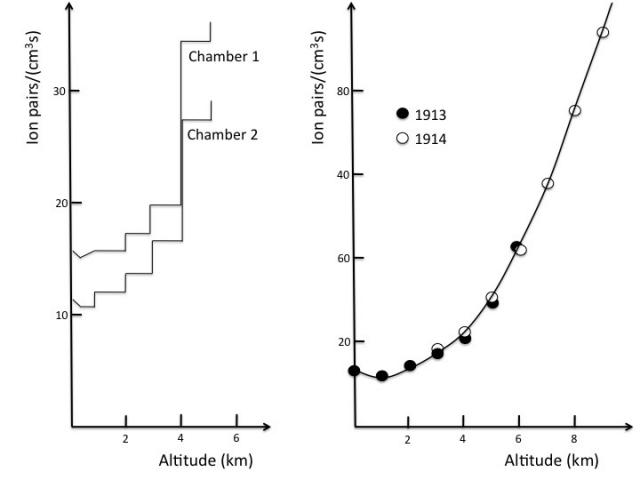
\includegraphics[width=0.7\textwidth]{figures/HessKol}
	\caption{Measurements of increasing ionizing radiation as a function of energy, by Hess in 1912 (left) and Kolhörster in 1913 (right), which provided strong evidence for an extra-terrestrial particle flux
	\cite{HessKolPic} }
\label{fig:HessKol}
\end{figure}
	
	\subsection{Cosmic Ray Physics and Cosmology}
	While the sources of cosmic rays remain unknown, their nature opens up the doors to many novel measurements of cosmological phenomenon that occur at extreme distances and energies.  Much of the universe is opaque to the traditional astronomical messenger particle, the photon, at high energies.  High energy gamma rays undergo electron-positron pair production in the presence of a magnetic field, effectively halting their travel before they can reach earth.(Figure \ref{fig:observableUniverse})\cite{RevModPhys.41.581}.  Additionally, the energies of some particles detected by cosmic ray observatories, on the order of $10^20$eV, dwarf the energies produced at terrestrial particle accelerators.  These particles can shed light on the world in the ultra high energy (UHE) regime.

\begin{figure}
\centering
	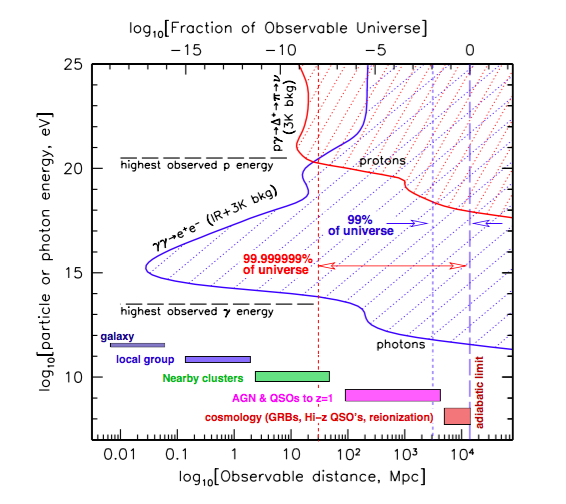
\includegraphics[width=\textwidth]{figures/ObservableUniverse}
	\caption{Interaction distances for photons and protons.  Shaded regions represent regions of the universe which are opaque to an astronomical particle. Credit to Dr. Peter Gorham for this plot.}
\label{fig:observableUniverse}
\end{figure}
	
	The observed energy spectrum of these hadronic particles introduces additional puzzles. As energy increases, the number of candidate sources for cosmic rays diminishes, leaving few to no intra-galactic candidates.\cite{RevModPhys.71.S33}  Flux density as a function of energy, shown in Figure \ref{fig:cosmicrayflux} is well measured up to the EeV energy scale with modern experiments, however in the UHE region, those particles with energies above $10^{18}$eV, statistical limitations caused by the incredibly low flux, on the order of 1/km$^2$/century, prevent accurate pointing to source locations.  Additional measurements are required to determine the transition between CRs emanating from galactic and extra-galactic sources.

	Using cosmic rays as a astronomical messenger particle presents new difficulties as well.  At lower energies, charged particles such as cosmic rays will have their courses altered by the Lorentz force while transiting the magnetic fields of stellar objects. Subsequently, inverting their incoming detection vector will no longer yield accurate pointing back to the source accelerator.  This is depicted in Figure \ref{fig:CosmicRayDeviation}.  Higher energy cosmic rays are proportionally less effected by magnetic fields due their increased rigidity, however, once more, the extremely low event statistics make it impossible to point to objects with any level of certainty. 
	
	The composition of cosmic rays at the highest energies remains under investigation as well.  An extensive air shower produced from a CR interacting with an atmospheric molecule has identical secondary detection characteristics whether the initial source particle was heavy ions or protons.  Recent measurements studying the maximum shower depth of air showers suggests a mixed composition, and possibly a hint at a transition from galactic to extragalactic source accelerator at EeV energies.\cite{AugerXmax}\cite{AugerXmaxDiscussion} Additional experimental observations of these cosmological particles will yield a better understanding of both the structure of matter and energy within the universe at large, as well as fundamental physics processes energetically unachievable from existing collider experiments.  The creation and propagation of ultra high energy cosmic rays through the universe opens a window to understanding of extreme high energy physics.

		
\noindent
\begin{figure}
\centering
	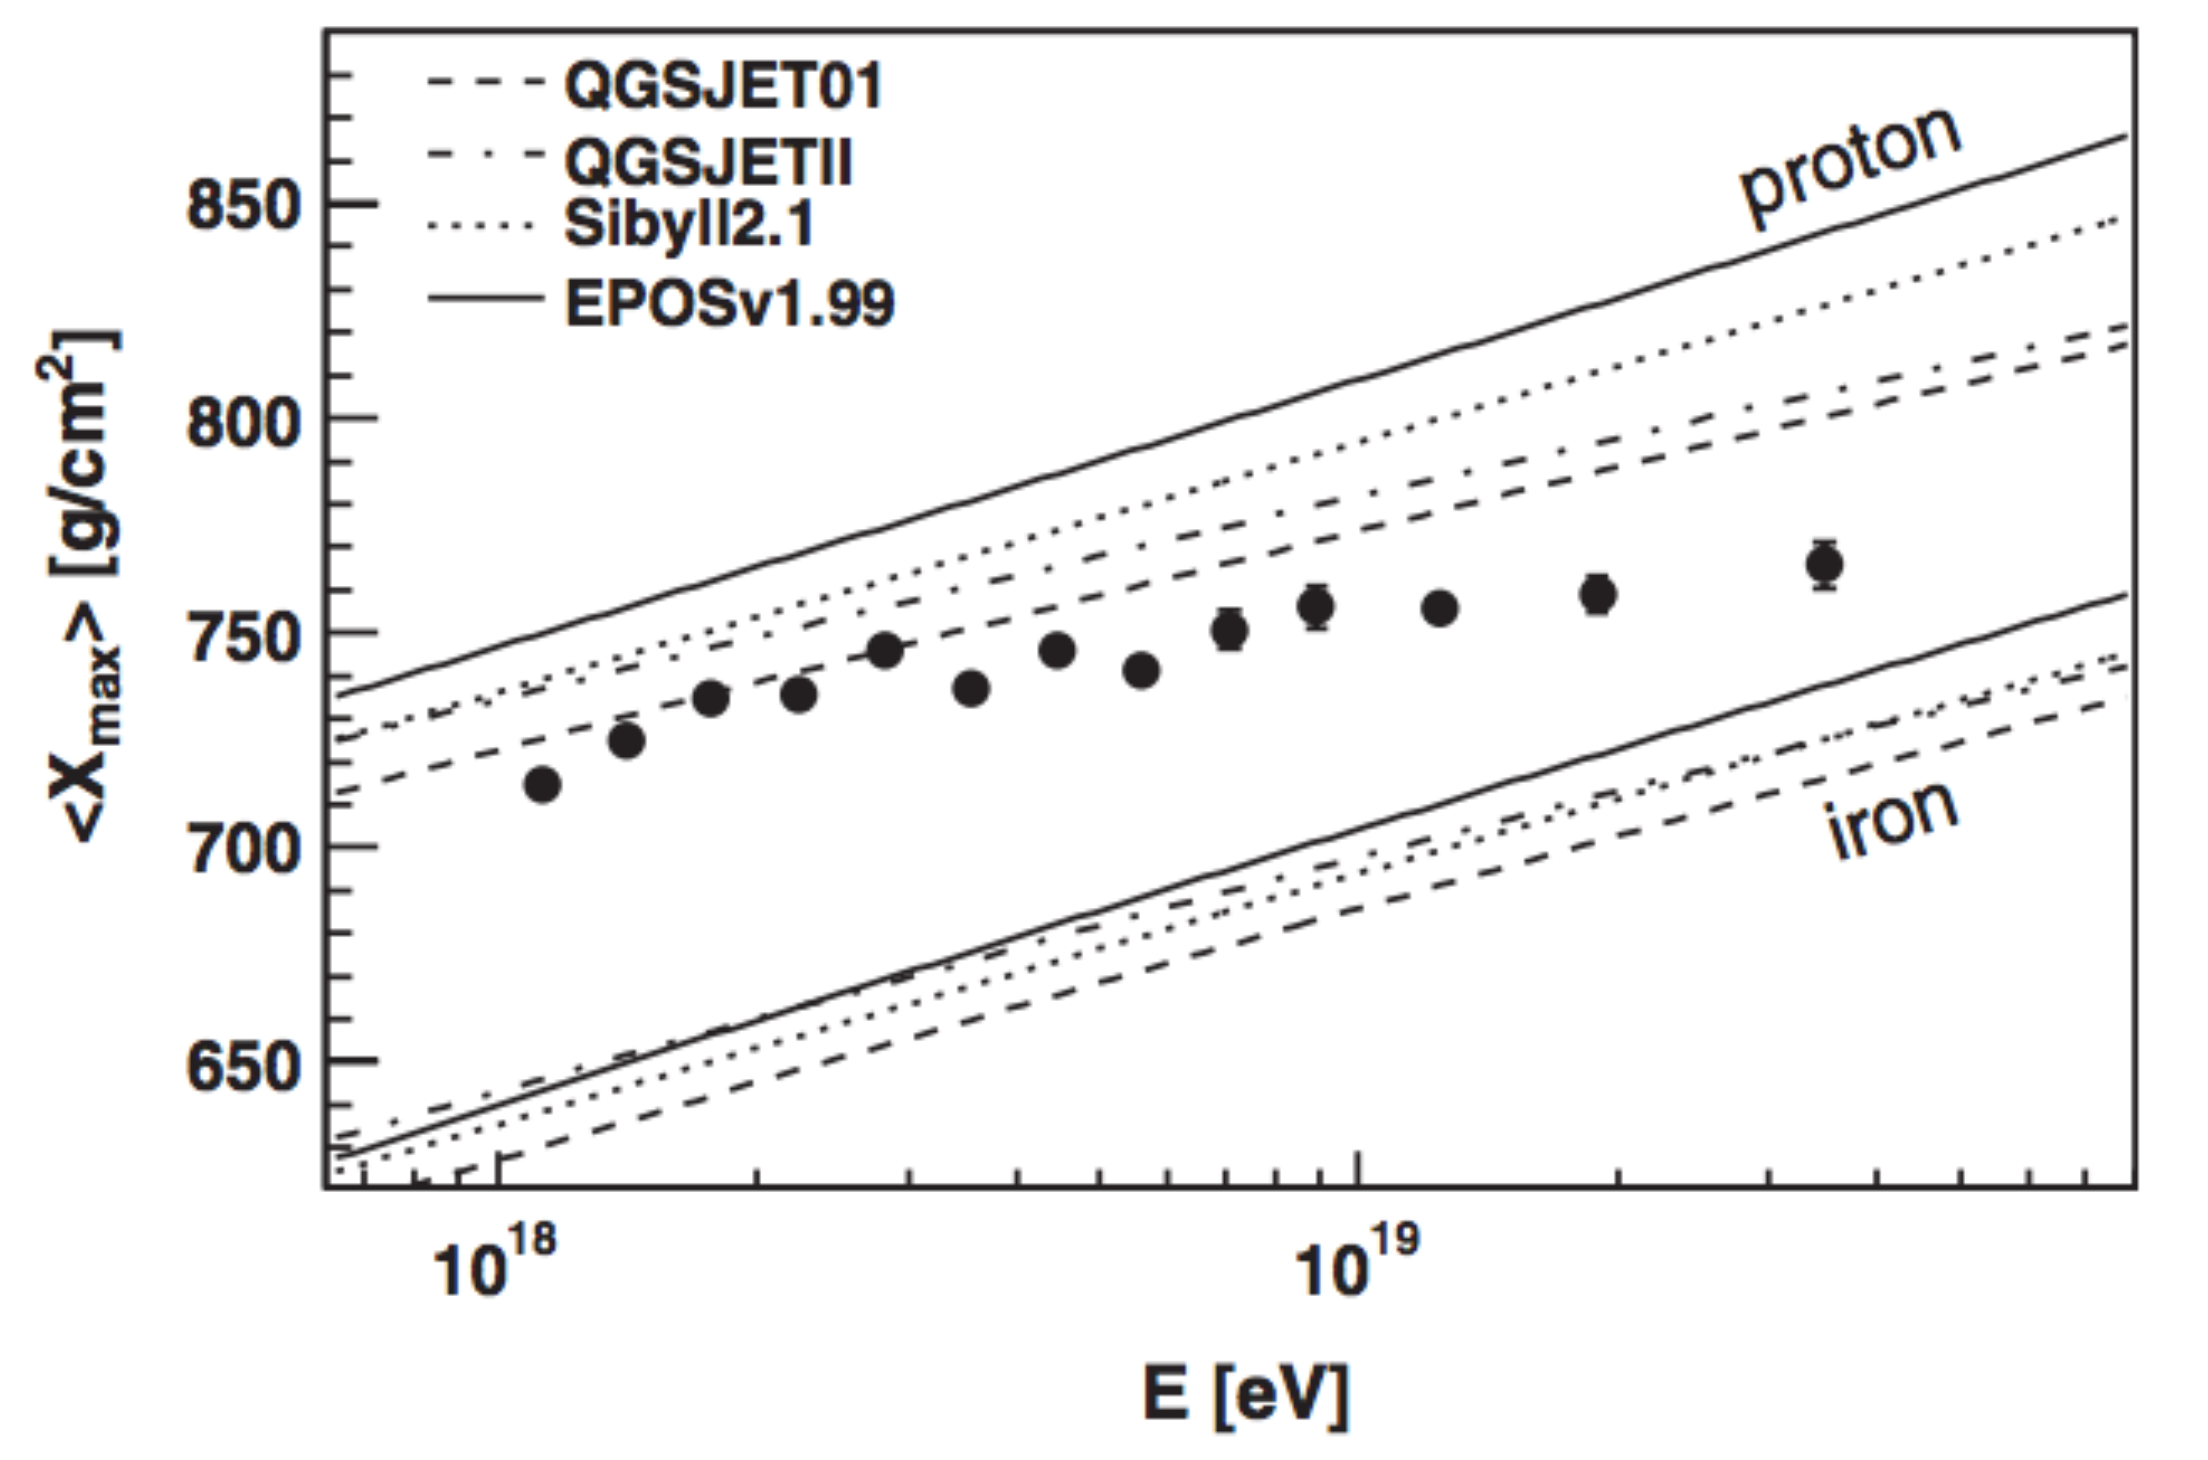
\includegraphics[width=\textwidth]{figures/AugerXmax}
	\caption{Measurements of cosmic ray maximum shower depth by the Auger observatory.  Modeled lines show theoretical predictions for two cosmic ray compositions, iron and protons\cite{AugerXmax}}
	\label{fig:AugerXmax}
\end{figure}

\noindent		
\begin{figure}
	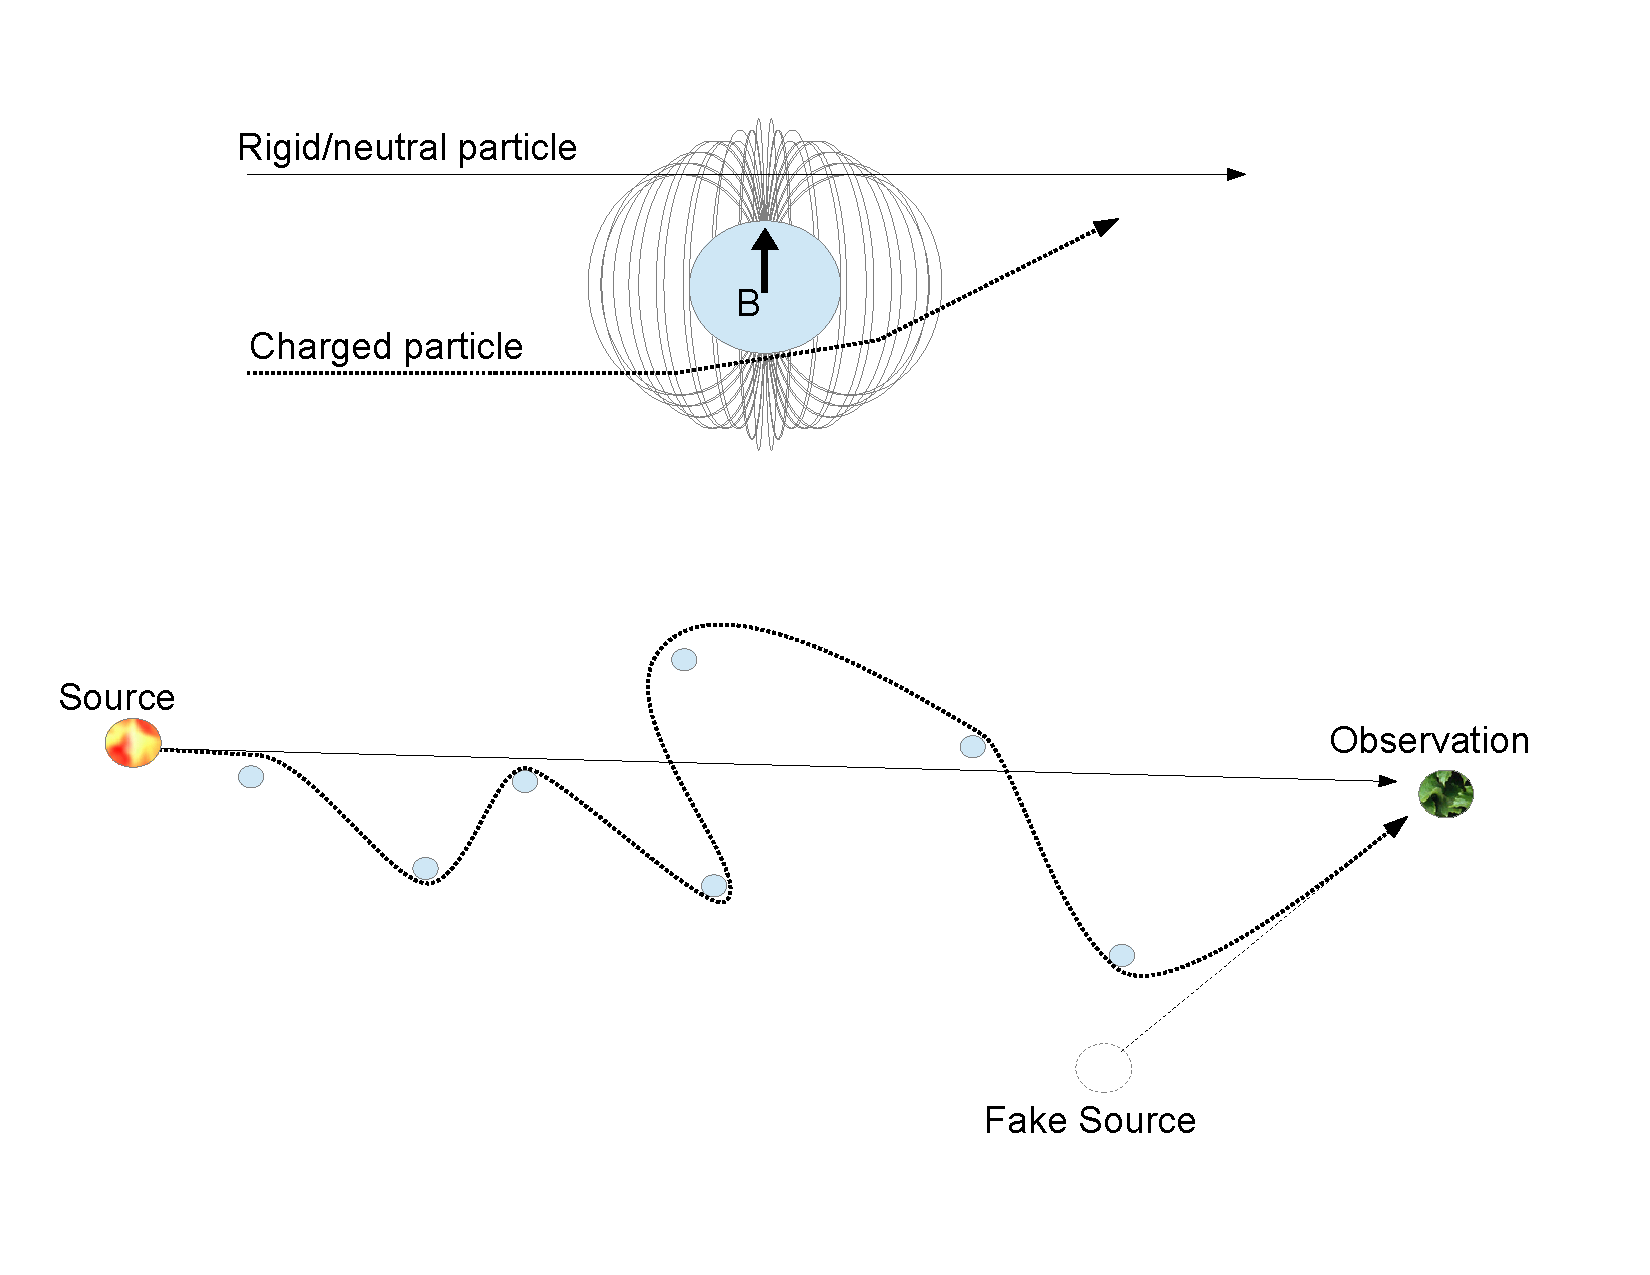
\includegraphics[width=\textwidth]{figures/CosmicRayDeflection}
	\caption{Top: A simplified diagram of lorentz-force induced curvature in low energy cosmic rays.  Bottom: An example of why magnetic deflection distorts the observed CR source location}
	\label{fig:CosmicRayDeviation}
\end{figure}
		

\noindent		
%\begin{wrapfigure}{L}{0.5\textwidth}
\begin{figure}
	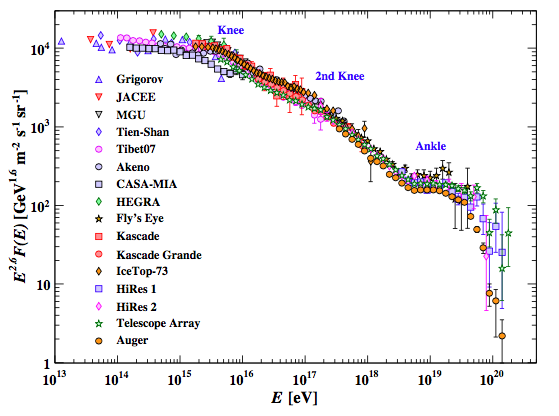
\includegraphics[width=\textwidth]{figures/CosmicRayFluxMeasurements}
	\caption{The all-particle spectrum as a function of energy-per-nucleus from measurements\cite{Olive:2016xmw}}
	\label{fig:cosmicrayflux}
\end{figure}
%\end{wrapfigure}		
		


\section{Neutrino astrophysics and the GZK interaction}
		The steep decline in observed flux measured by detectors alludes to an interaction mechanism that opens up a new detection prospect for cosmic rays.  Dubbed, "the ankle" in Figure \ref{fig:cosmicrayflux}, the sharp decrease at 10$^{19}$eV corresponds to an interaction of a rest proton with a high energy gamma ray through a delta resonance.  Shifting the frame of reference to a relativistic proton colliding with a low energy photon, one arrives at an accurate description of a cosmic ray transiting the cosmic microwave background (CMB) radiation that isotropically pervades the universe.\cite{WMAPCMBResults}  This interaction was predicted by Greisen–Zatsepin–Kuzmin, and represents a theoretical high energy limit on particles coming from outside of the galaxy, known as the GZK limit, at 5x10$^{19}$ eV, above which particles will scatter off the CMB and decline in energy.\cite{GZK}  Observatories measuring UHE cosmic rays have detected a decrease in the quantity of observed particles consistant with a GZK induced suppression.\cite{GZKMeasurement} Cosmic ray particles were also observed exceeding this limit however, suggesting an intra-galactic source of unknown origin.  The low statistics of particles observed at this energy prevent identification of a specific source.  Since particles are present at these high energies, it would also be expected that other regions of the universe also contain accelerators capable of creating cosmic rays in excess of the GZK limit, thus motivating a UHE neutrino flux.
		
		The GZK process has multiple channels, each of which produce an ultra high energy neutrino (UHE$\nu$) messenger particle that could subsequently be detected on earth (Figure \ref{fig:GZKDiagram})\cite{GZK}.  Though the flavor ratio produced in a GZK interaction is not equally distributed, flavor oscillation during their long time-scale traverse to earth will result in an observable flavor ration of 1:1:1.  The cross section of neutrinos has been measured in accelerator facilities to be vanishingly small at modern accelerator scale energies.\cite{neutrinoCrossSectionMeasurements}  However, at energies out of reach of modern accelerators, cosmic accelerators could illuminate our understanding of neutrino cross section.  The neutrino cross section at energies above those measured by accelerator facilities has been estimated by using standard model particle physics.\cite{neutrinoCrossSectionExtrapolation} This small cross section allows the GZK interaction messenger neutrino to traverse unimpeded through the interstellar medium before subsequently interacting with earth.  Additionally, the uncharged nature of neutrinos allow them to travel in a straight line from their source locations without Lorentz deflection from intervening magnetic fields.  Cosmologically propagating neutrinos have an extremely small cross section, such that their path length through empty space is essentially infinite, allowing an unparalleled view into the depths of the cosmos.

\noindent		
%\begin{wrapfigure}{L}{0.5\textwidth}
\begin{figure}
	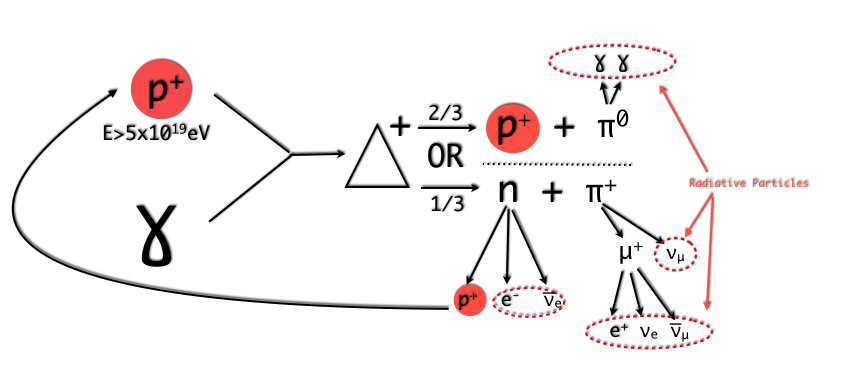
\includegraphics[width=\textwidth]{figures/GZKDiagram}
	\caption{A diagram of the possible resultant particles of a GZK interaction between a photon and the CMB.}
	\label{fig:GZKDiagram}
\end{figure}
%\end{wrapfigure}		
			
		
	\subsection{Unexplained UHE Source Mystery}
		Though there are numerous cosmic ray sources that have strong theoretical motivation, above 10$^{17.5}$eV the number of candidates becomes constrained and an extra-galactic source hypothesis becomes required. \cite{RevModPhys.71.S33}  Due to the higher flux of nearby low energy cosmic ray sources, many experiments have gathered evidence to support source candidates within our galaxy as accelerators.  However, above the GZK suppression limit there remains little collected experimental evidence that describes the transition to extra-galactic sources. These higher energy objects include such objects and Active Galactic Nuclei (AGN), supernova, quasars, gamma-ray bursts, as seen in Figure \ref{fig:cosmicAccels}  However, the small statistics afforded by incident particles at the EeV end of the spectrum makes identifying their acceleration mechanisms much more difficult, and requiring extremely large detector volumes.

\begin{figure}
	\centering
	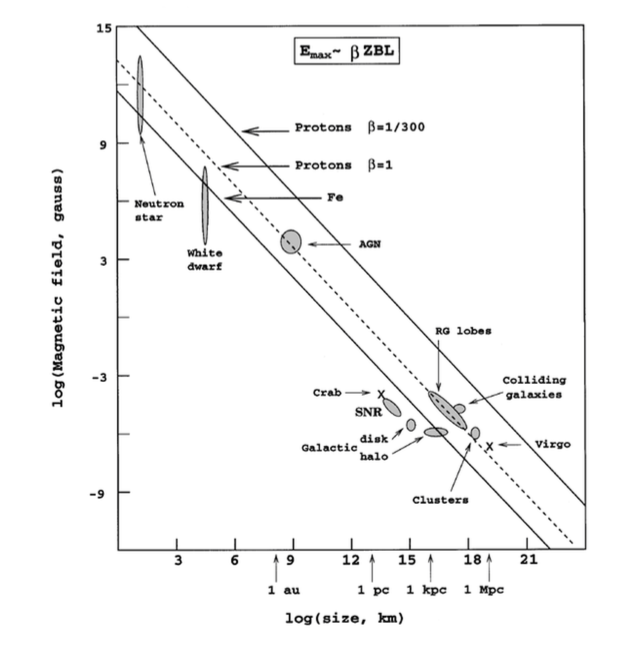
\includegraphics[width=\textwidth]{figures/cosmicAccelerators}
	\caption{Theorized cosmic accelerators plotted by their size and peak magnetic field.  The dashed line denotes 
a field strength capable of accelerating protons to $10^{18}$ eV. \cite{RevModPhys.71.S33} }
	\label{fig:cosmicAccels}
\end{figure}


\section{Neutrino Detection on Earth}
	The neutrinos produced in GZK interactions are messenger particles that carry information about UHECRs produced outside the galaxy to earth at energies above the GZK suppression effect.  Astronomical neutrino telescope observations have been carried out at lower energies nearly since the discovery of the particle itself. Recently however, there has been a notable increase in detector scale and energy sensitivity.  Since the term "cosmic ray" describes any high energy particle incident on earth (including gamma rays), for the purposes of this dissertation, neutrinos fit the description of cosmic rays.
	
	The largest notable difference between observations of UHE neutrinos and cosmic rays is the medium in which they are most likely to interact.  While cosmic rays have large cross sections and are predicted to interact with even low density media, such as the atmosphere, neutrinos require a medium with far higher density.  Interestingly, both particle interaction lengths can be described with a traversed density unit, or specifically for the case of cosmic rays the atmospheric depth, $\frac{g}{cm^{2}}$.  For UHE$\nu$s however, this term becomes larger than the integrated total density of the atmosphere regardless of incoming slant angle.  The neutrino will therefore either skim the atmosphere entirely if shallow enough, or interact within the earth if too steep.  However, if a dense dielectric solid is introduced or utilized at the Earth's surface by an opportunistic experimenter, it is possible to capture neutrino interactions within the field of view of detection equiptment.  This equiptment can capture the induced electromagnetic showers from a high energy particle shower.
	
	\subsection{Charged current and Neutral Current interactions} 
		Neutrinos have two distinct interaction classifications, neutral current and charged current.  A neutral current interaction occurs through the exchange of a $Z^{0}$ particle, and transfers some of its energy and momentum to the particle it interacted with.  A charged current interaction involves the exchange of a $W^{\pm}$, and results in the neutrino being converted into the a similarly flavored and charged lepton.  The two interactions have differing cross sections and have different characteristic signals.
				

	\subsection{Extensive Air/Ice Showers}
		A highly energetic particle interacting with the hadronic matter present in Earth's atmosphere, or in any  dense material, creates an extended series of particle production, scatterings, and decays.  This extensive shower of particles scattered and created from a single extra-terrestrial high energy source particle has been appropriately dubbed an Extensive Air Shower (EAS).  These showers produce both traveling messenger particles that can be observed through weakly interacting secondary scatterings in instrumented transparent scintillating media, as well as through primary radiation, which is the topic of this thesis.  This primary radiation is stimulated by the appearance of moving charged particle pairs that travel along the principle shower axis.  There are two main electromagnetic radiative effects, detailed below and depicted in Figure \ref{fig:EASRadiation}, that can be observed in the  VHF (3MHz to 300MHz) and UHF (300MHz to 3GHz) bands of the electromagnetic spectrum.  This region of the spectrum has very good transmissive properties in the atmosphere, as well as within many dense solids.\cite{Besson2009348}\cite{VuFind-000215473}\cite{Barrella:2010vs}
		

\begin{figure}
	\centering
	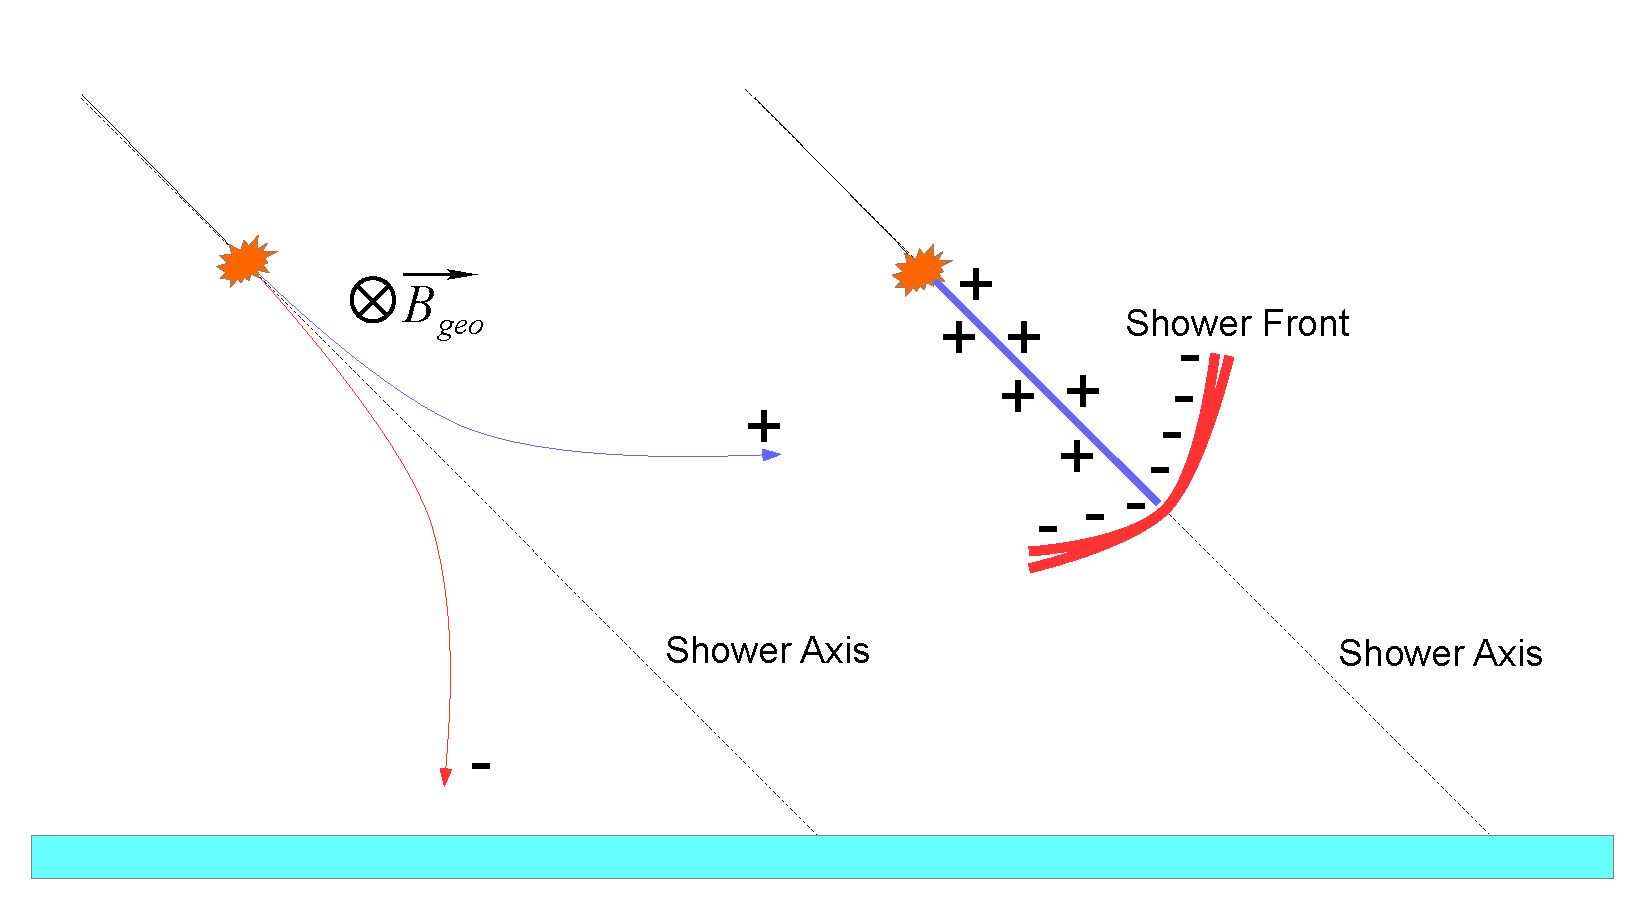
\includegraphics[width=\textwidth]{figures/EASRadiation}
	\caption{Simplified schematic of two EAS radiative trasmission mechanisms, geomagnetic (left) and charge-excess, or Askaryan, radiation (right)}
	\label{fig:EASRadiation}
\end{figure}

	
	\subsection{Geomagnetic Radiation}
		The primary and strongest radiative effect in an EAS is from a longitudinal charge separation created from a Lorentz force as the newly created grouping of charged particles move through the geomagnetic field of the Earth.  As the shower is required to have zero net charge (A CR will have a total incident charge of +1 and a neutrino has none), an equal number of positively and negatively charged particles is expected to be generated.  The Lorentz force, $F=q(\vec{E}+\vec{v}\times\vec{B})$, acting on oppositely charged particles will move them in opposite directions, inducing a spacial separation.  This charge separation emits radiation with a linear polarization orthogonal to the magnetic field and the shower axis with an intensity proportional to the incoming shower energy and magnetic field.
	\subsection{Askaryan Effect}
		A secondary radiation component, theorized by Gurgen Askaryan in 1962, as a build up of negative charge at the front of the shower core as electrons are created and scattered forward, while their positron pairs are annihilated.\cite{Askaryan:1962hbi}  This creates a charge separation between the negatively charged shower front and the positively charged shower path.  This relativistic velocity charge buildup will radiate coherently at critical off angles where their created wavelengths constructively interfere.  This is visible as a sharp broad spectrum impulse, as a stationary viewer observes a enormous charge flux.\cite{PhysRevD.84.103003}  This effect has much more recently been measured at particle accelerators in a variety of materials, including ice,\cite{PhysRevLett.99.171101} salt\cite{PhysRevD.72.023002}, and silica sand\cite{PhysRevLett.86.2802}.  An example accelerator initiated Askaryan pulse in ice measured by the ANITA electronics is visible in Figure \ref{fig:ANITASLACPulse}
		
		
\begin{figure}
\centering
	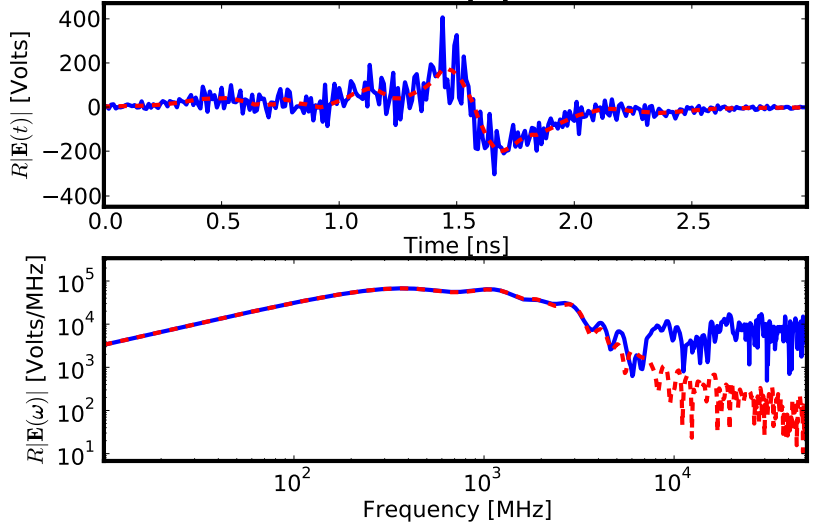
\includegraphics[width=\textwidth]{figures/AskaryanSimulation}
	\caption{The electric field of an Askaryan pulse observed close to the critical angle in the far field generated by a mathematical model(red), and with the ZHS simulation package(blue) \cite{PhysRevD.84.103003} }
	\label{fig:AskaryanSimulation}
\end{figure}

\begin{figure}
\centering
	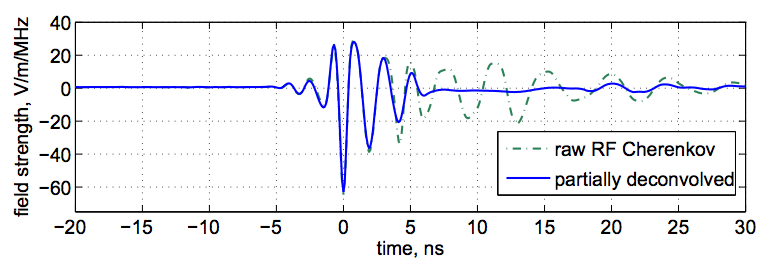
\includegraphics[width=\textwidth]{figures/ANITASLACImpulse}
	\caption{An example accelerator initiated Askaryan pulse in ice measured by the ANITA electronics  The dispersion in the signal is introduced by the band-pass filtering in the RF signal chain\cite{PhysRevLett.99.171101} }
	\label{fig:ANITASLACPulse}
\end{figure}


	\subsection{Cherenkov Radiation}
		Considering a realistic index of refraction for the dielectric medium in which a particle shower occurs results in a boost to both primary sources of shower radiation at distances slightly off the shower axis.  This is caused by constructive interference induced by the relativistically propagating shower through a dielectric, in which light propagates at $<c$, at a critical off angle, which corresponds with Cherenkov radiation.  This process is shown in Figure \ref{fig:Cherenkov}.
		

\begin{figure}
\centering
	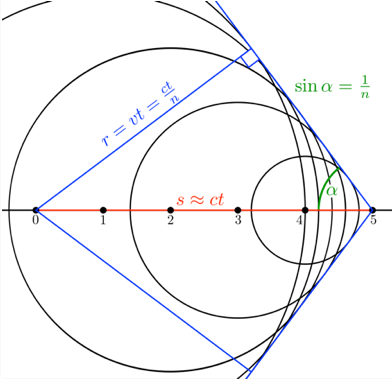
\includegraphics[width=0.5\textwidth]{figures/Cherenkov}
	\caption{An example diagram of the Cherenkov critical angle where the radiative components of a CR shower experience a signal boost.}
	\label{fig:Cherenkov}
\end{figure}


	\subsection{Tau-$\nu$ Specific Detection Prospects}
		Though the Earth becomes opaque to neutrinos at high energies, secondarily created particles such as a Tau lepton from a similarly flavored neutrino undergoing a charged-current interaction have a regeneration effect that opens a larger field of view than just the sliver of ice at the horizons.  These Taus, which have a relatively short half-life, will then decay in the atmosphere, initiating an EAS that travels upwards from the surface of the Earth.  A tau neutrino thus has a higher accepted incoming angle, as it can traverse further through the dense rock of the Earth without being absorbed fully.  A UHE$\nu_{\tau}$ will behave characteristically similar to a UHECR, except that it will have a flipped polarity to a reflected down-going EAS, and a matched polarity to a directly viewed EAS.  A search for UHE$\nu_{\tau}$ particles was done for the ANITA1 data set, and furthering the search for the ANITA3 flight is a primary motivator of this thesis.  This "double-bang" tau neutrino interaction has been simulated, and other experiments are searching for their signals\cite{PhysRevD.86.022005}. 

\section{ANITA}
	Up to this point, I have mainly motivated a detectable physics hypothesis from established theories and measurements.  From here, I can introduce a detection platform for these physics phenomenon, the ANtarctic Impulsive Transient Antenna (ANITA).  EASs present in the atmosphere or in the dense, radio transparent, dielectric solid ice sheet covering the souther continent of Antarctica will produce unique and characteristic signals through the above particle interactions and radiative effects.  A high altitude, long duration, telescope platform would have an extremely large field of view, thus increasing the possibility of observing one of these rate interactions.  Additionally, downwardly moving atmospheric CR shower events can be both observed by the payload directly, or as reflections off the ice that covers the Antarctic continent.  These reflected pulses will have an inverted phase from the theoretical models of an EAS.  The following chapters detail the instrument, analysis, and simulation of the third ANITA flight.





%%%%%%%%%%%% 2 %%%%%%%%%%%%%%%%%%%%%%%%%%%%%%%%%%%%%%%%%%%%%%%%%%%%%%%%%%%%%%%%%%%%%%%%%%%
\chapter{ANITA Telescope Platform}
%%%%%%%%%%%%%%%%%%%%%%%%%%%%%%%%%%%%%%%%%%%%%%%%%%%%%%%%%%%%%%%%%%%%%%%%%%%%%%%%%%%%%%%%%%
\section{Overview}
	The ANITA telescope platform is a passive broad-band radio frequency electromagnetic field transient detector and time domain voltage digitizer.  There have been four ANITA flights at the time of this thesis, numbered one through four.  ANITA1 flew in the 2006-2007 Antarctic balloon campaign\cite{ANITA1}, ANITA2 in 2007-2008\cite{ANITA2}, ANITA3 in 2014-2015 (the topic of this thesis) and most recently ANITA4 in 2016-2017.  
	
	The main instrument structure consists of a collection of radially positioned, outwardly facing, broad-band, highly-directional quad-ridge horn antennas.  The antennas are separated into three different vertically spaced rings, with each ring separated into 16 different azimuthally facing "phi-sectors." (see Figures \ref{fig:phiSectors} and \ref{fig:ANITA3_hangtest})    These co-pointing antennas allow multiple observations of a signal event with a physical distance baseline offset between them. These antennas couple the incident electromagnetic radiation into a coaxial signal line, which is then amplified by a series of low noise-figure amplifiers, band-pass filtered via analoge compound filters into the relevant frequency bandwidth, before finally being digitized by custom on board high-speed digitizer chips and readout electronics (Figure \ref{fig:RFChainBlockDiagram}).  The digitization is self-triggered by a parallel square-law integrating power detector circuit which arrives at a decision with minimal analog waveform buffering.  After digitization, waveforms are read out via a CPCI interconnect backplane to a ruggedized conductively cooled CPU writing to on-board redundant storage devices.  The payload is capable of reading out ~50Hz of full payload waveforms with low (\textless 5\% ) deadtime to disk.  Additional position and orientation data, as well as multiple diagnostic and in-situ relevant physics measurements, are recorded and precisely time-stamped by a GPS disciplined clock.  Selections of the waveforms and housekeeping measurements are telemetered down to ground servers for in-flight diagnostics, however full recovery of the data vaults is desired for a complete analysis.  The following chapter will expand upon these systems and the theoretical basis for their design and construction.
	
	
\begin{figure}
\centering
	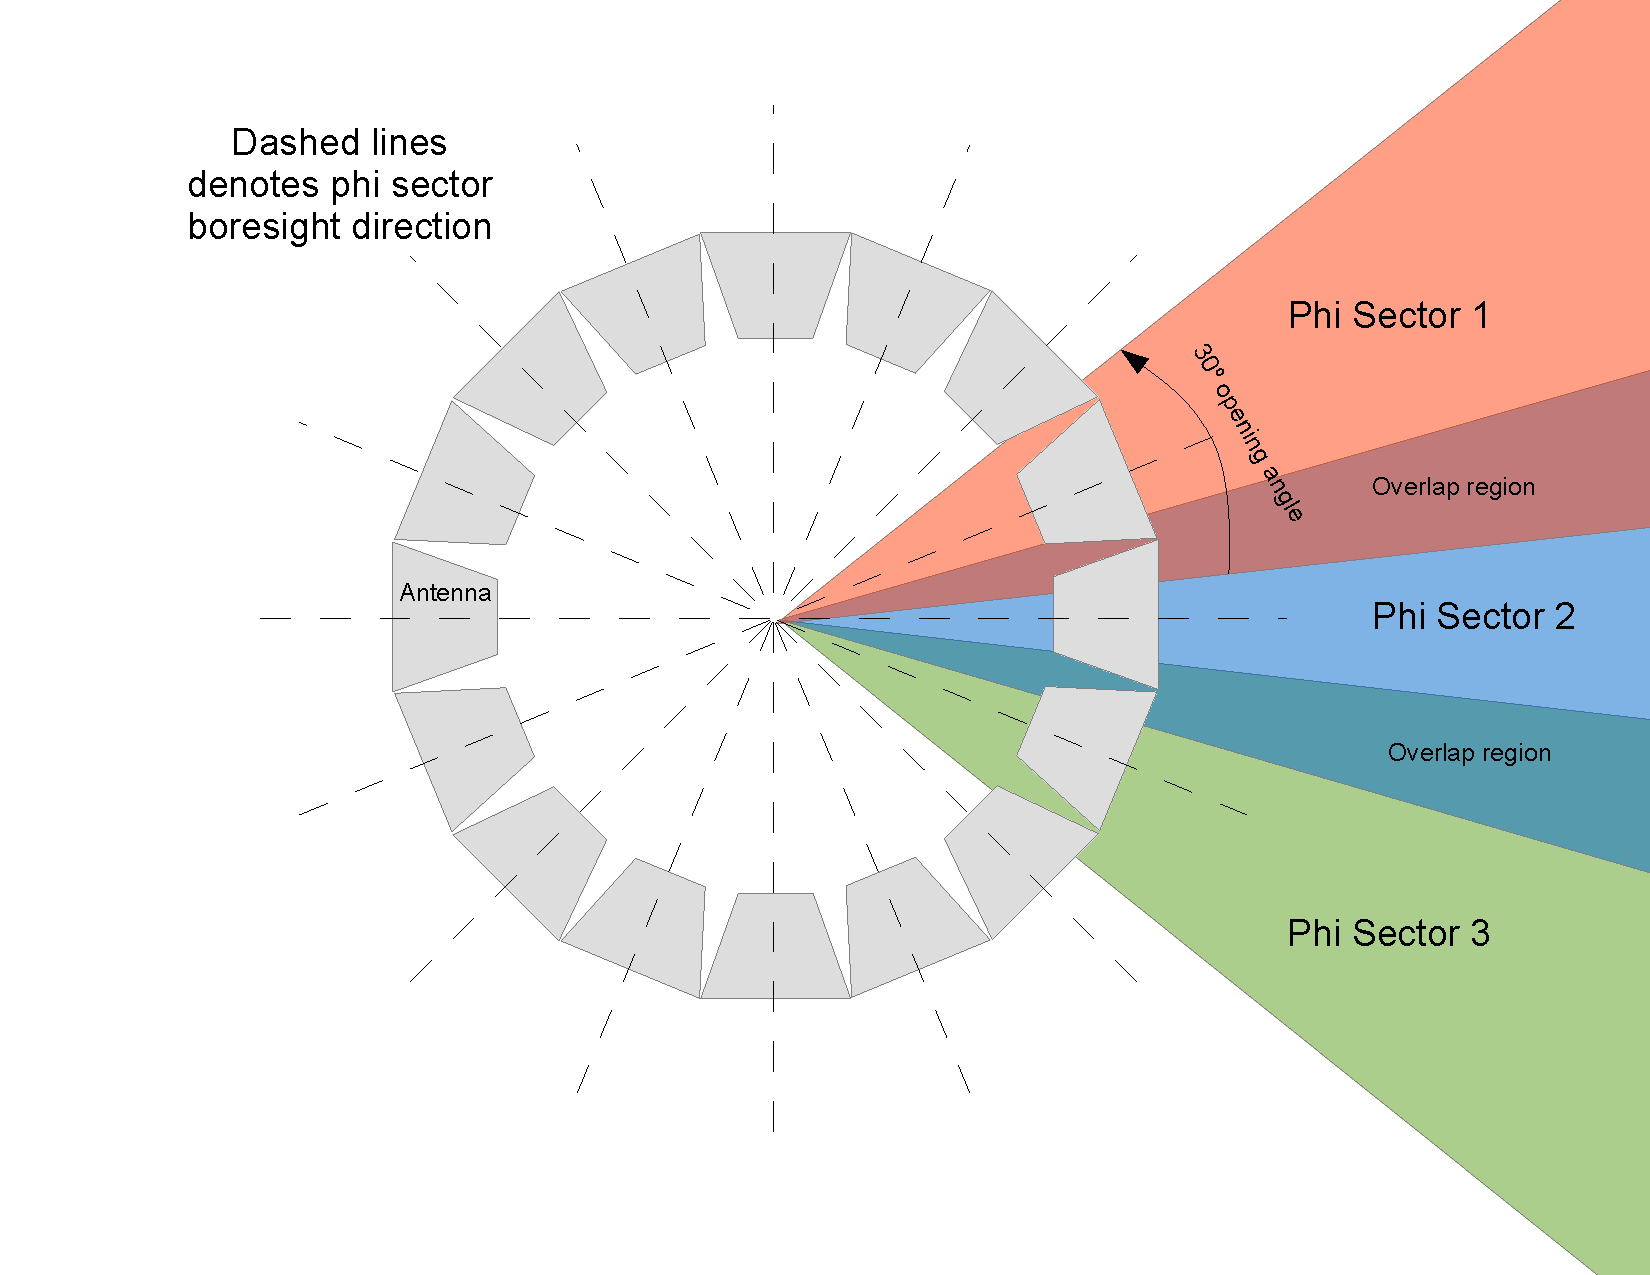
\includegraphics[width=\textwidth]{figures/phiSectors} 
	\caption{A top down diagram depicting a single ring layout of the horn antennas used to achieve complete azimuthal coverage assuming a 30$^{\circ}$  opening angle.  The antenna gain pattern is discussed further in the Calibration section.}
	\label{fig:phiSectors}
\end{figure}

	
\begin{figure}
\centering
	\includegraphics[height=0.9\textheight]{figures/ANITA3_hangtest2_annotated}
	\caption{An image of the ANITA3 telescope during the test deployment in Palestine TX, 2014.  Marked from top to bottom are two of the nine GPS antennas, the three vertically separated rings, the deployed solar panel array, and a deployed ALFA antenna.  The solar panels visible at the top of the payload are those used by the NASA Small Instrument Package (SIP).  Not visible are the ANITA instrument crate and other objects on the deck of the experiment (between middle and top antenna rings).}
	\label{fig:ANITA3_hangtest}
\end{figure}

\begin{figure}
\centering
	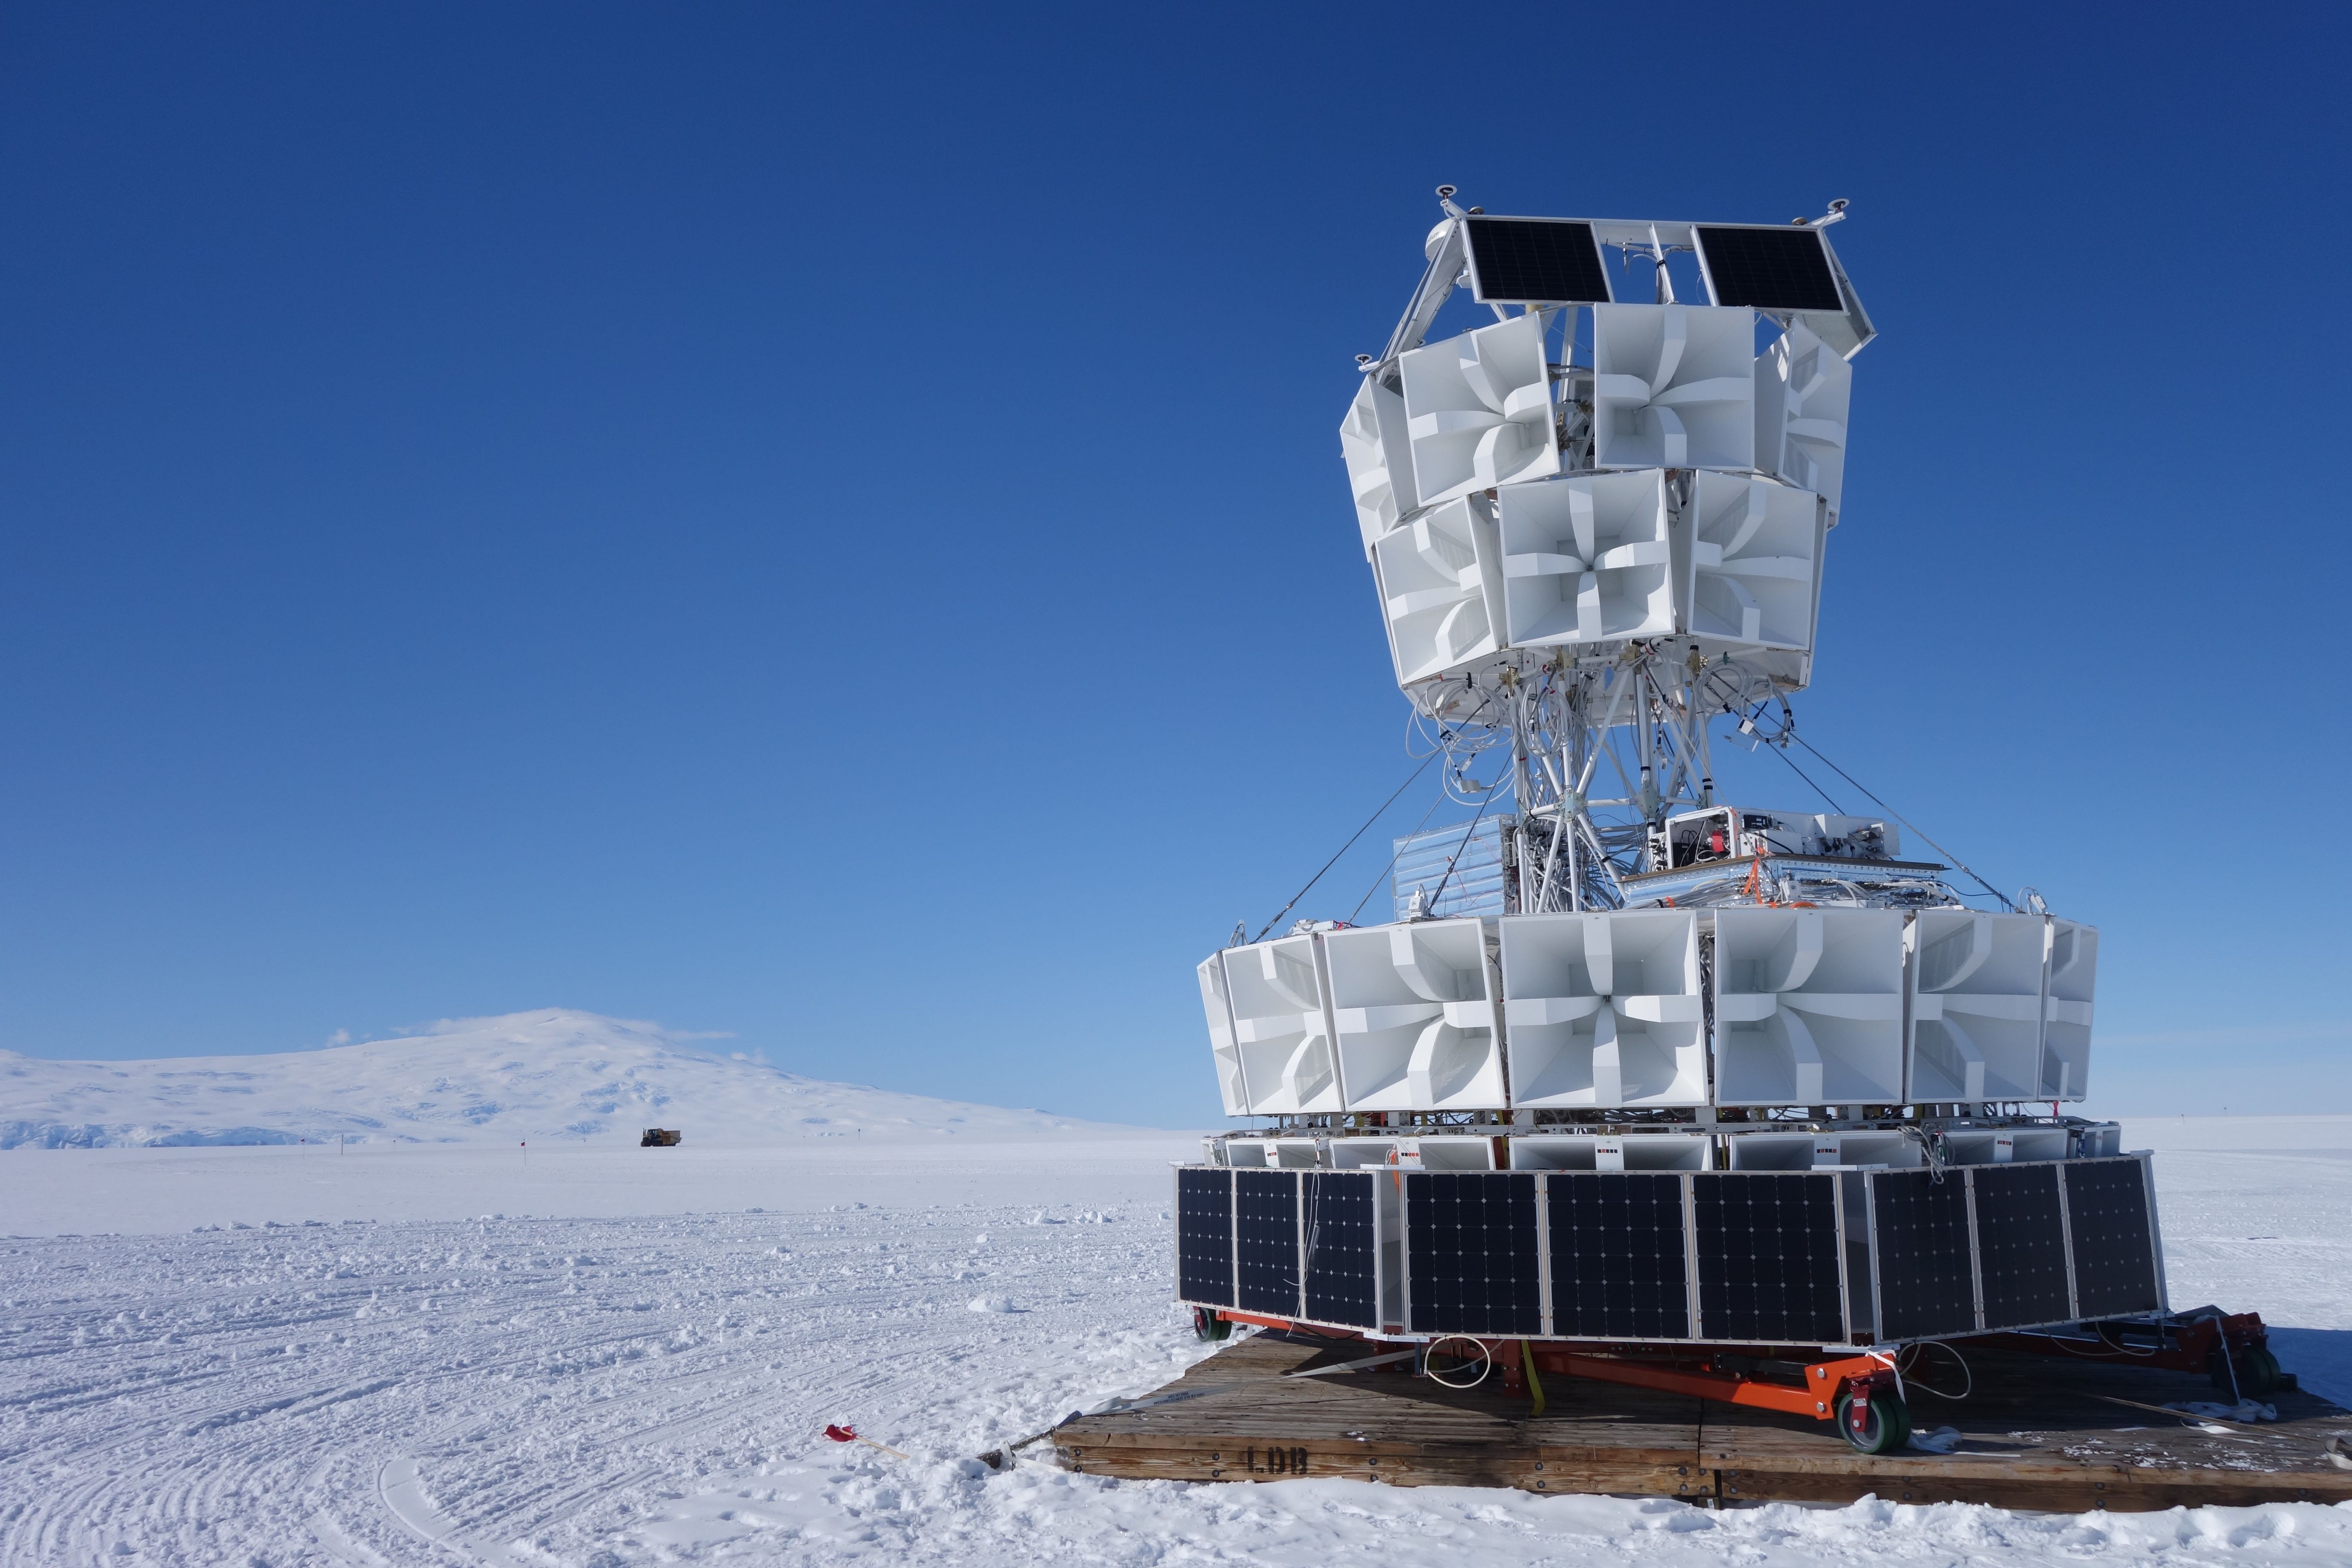
\includegraphics[width=\textwidth]{figures/ANITA3_dancefloor}
	\caption{An image of the ANITA3 during GPS calibration on the "dance-floor" at the Long Duration Balloon (LDB) facility at McMurdo Station in Antarctica prior to launch in 2014.  In the background is Mt. Erebus.  In this image the solar panels are in their retracted state, the instrument crate is visible on the left hand side of the central column, and the NASA Small Instrument Package (SIP) is visible on the right hand side. The orange structure seen under the payload is a stand used during construction and testing of the instrument.}
	\label{fig:ANITA3_dancefloor}
\end{figure}

\begin{figure}
\centering
	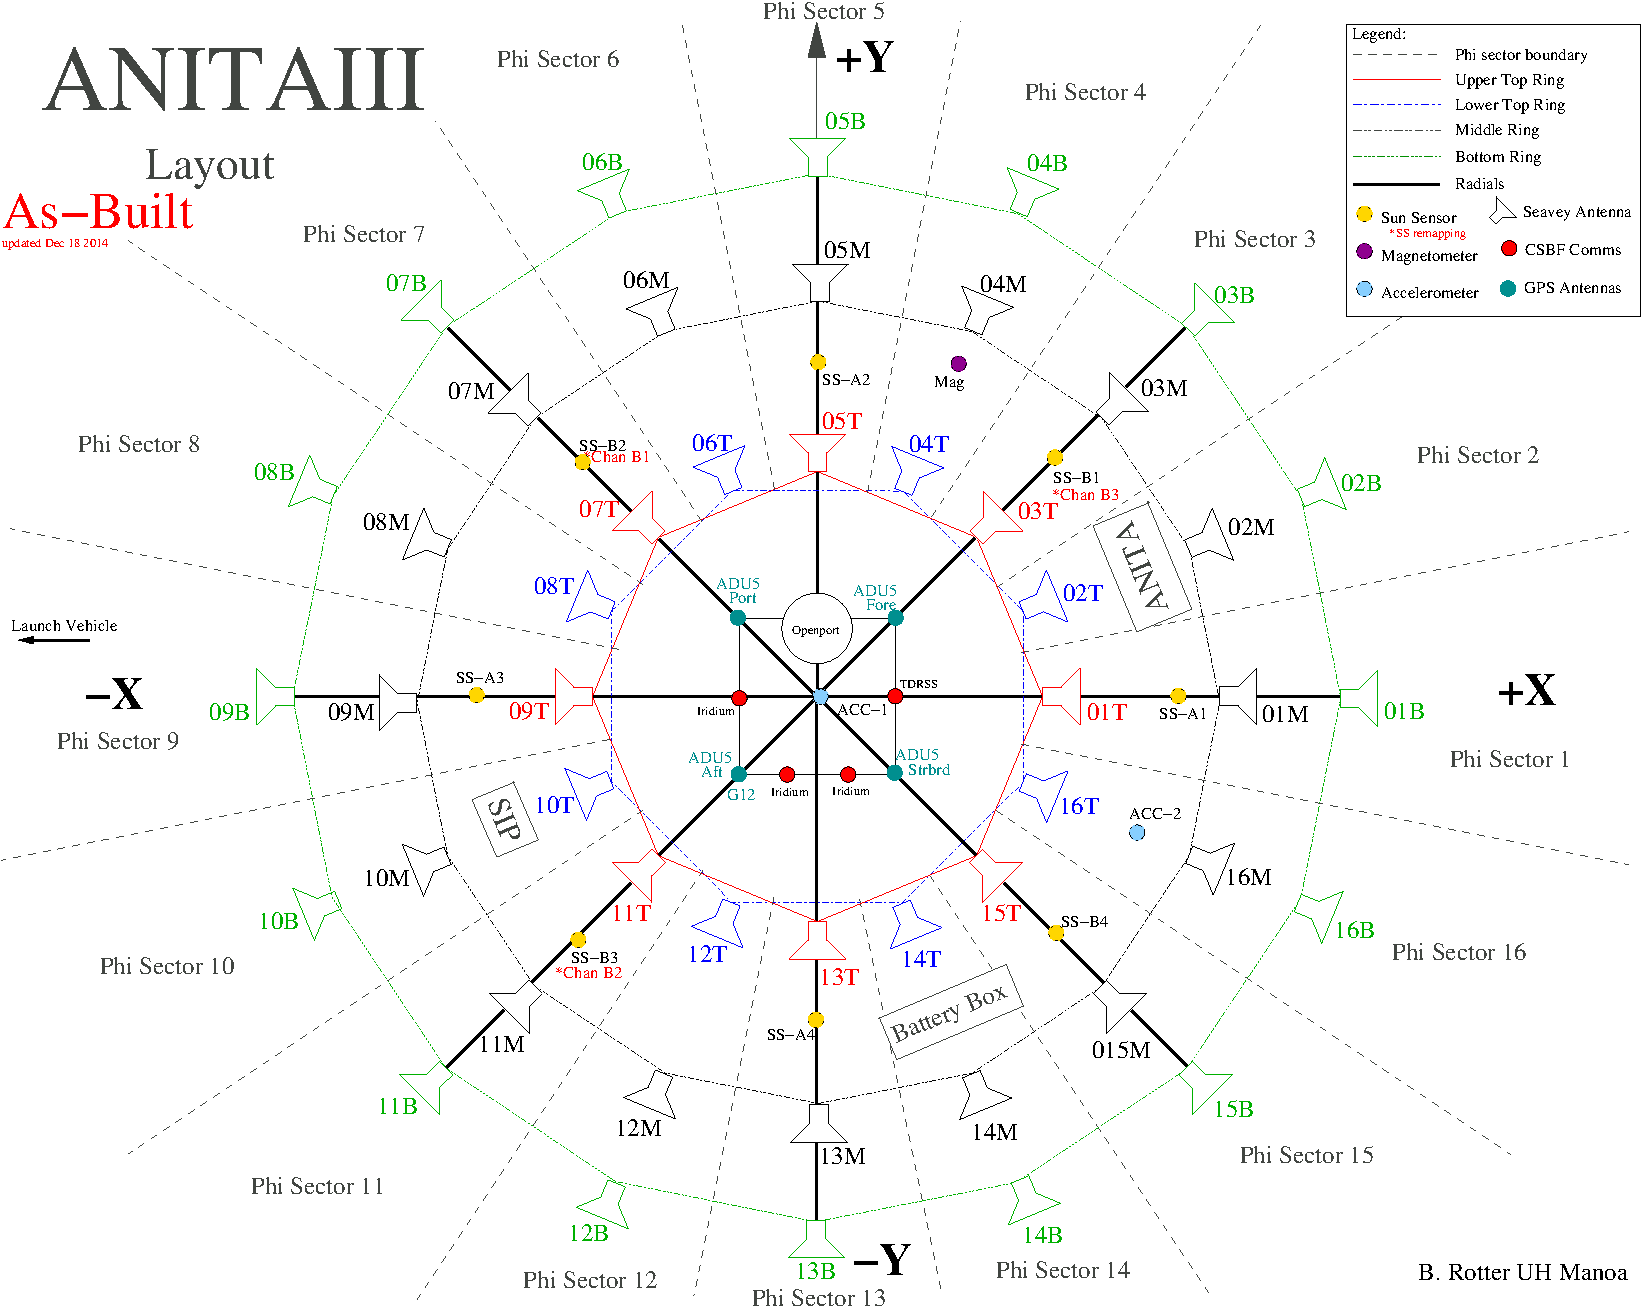
\includegraphics[width=\textwidth]{figures/ANITA3_layout_asBuilt}
	\caption{A top-down diagram detailing the locations of various components on the ANITA3 instrument as it was flown.  Visible are the locations of the NASA Small Instrument Package (SIP) and ANITA instrument box as they relate to the GPS antennas and measurement antenna phi sectors.}
	\label{fig:ANITA3_asBuilt}
\end{figure}

\begin{figure}
\centering
	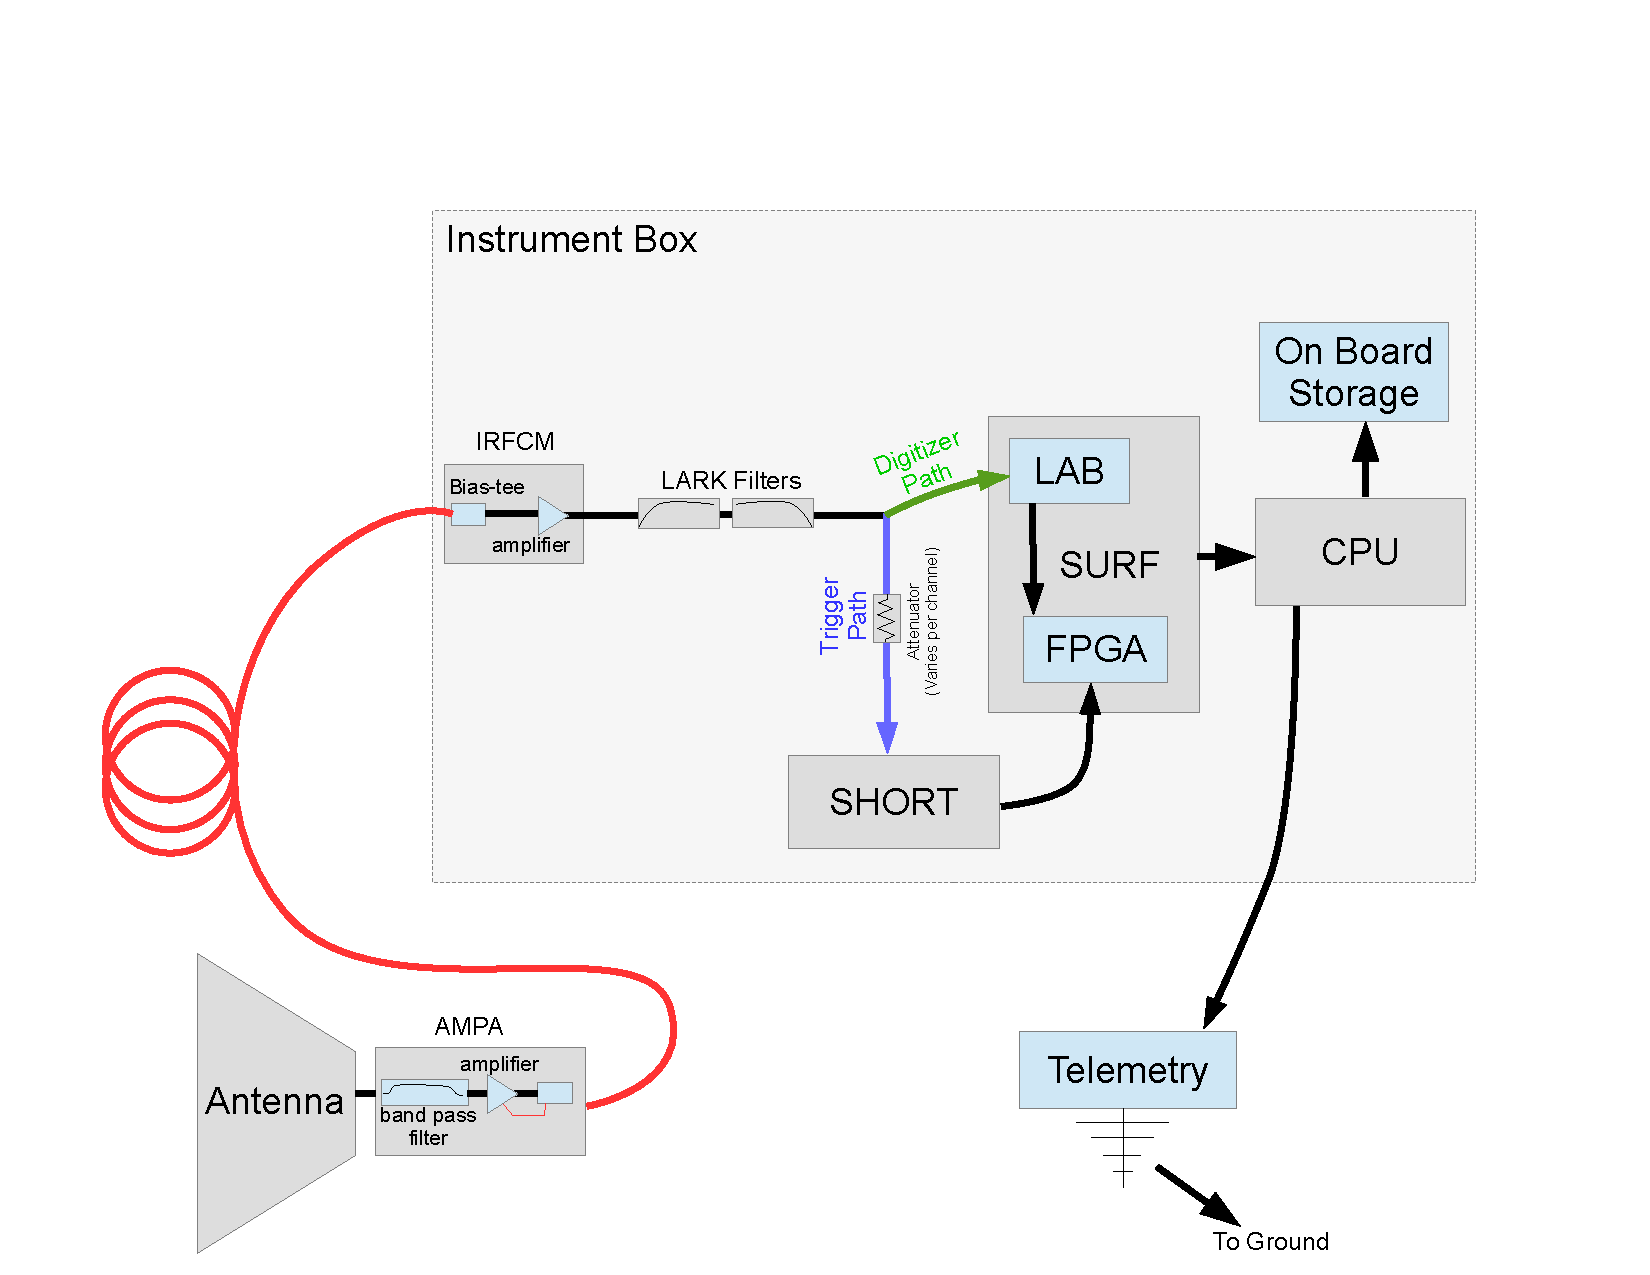
\includegraphics[width=\textwidth]{figures/RFChainBlockDiagram}
	\caption{A simplified diagram of the ANITA3 signal chain from antenna to data storage or telemetry.}
	\label{fig:RFChainBlockDiagram}
\end{figure}

	
\section{Antennas}
	The ANITA instrument's main science mission utilizes dual polarized quad ridge horn antennas to convert the electromagnetic field incident on the payload into an electrical signal that can be digitized and stored for later analysis.  The antennas design specifications include a flat gain and phase response over the full gigahertz of bandwidth, high directionality in order to reduce noise and boost signal fidelity, two orthogonal polarizations with co-located phase centers, and light weight.
	
	ANITA1 began with only two vertically separated rings and 32 antennas, however subsequent flights have packed more into the available space dictated by the flight vehicle launch envelope.  Between ANITA1 and ANITA2 an additional eight deployable nadir ring antennas were added that unfolded into flight position immediately after launch.  Between ANITA2 and ANITA3 an additional 8 antennas were added to the lower ring, equalizing the number per phi sector and bringing the total count to 48.  ANITA4, being a fast-turn-around re-flight, flew the same number of antennas as ANITA3.
	
	Antennas are located to maximize baseline distance between pairs pointing at similar regions of the field of view in order to maximize angular resolution recovered from interferometric pointing.  The benefits of increased baselines are discussed further in the calibration chapter.  The additional antennas added in each ANITA flight increase not only the number of baselines possible for this interferometric pointing, they provide an additional $\frac{1}{\sqrt{N}}$ incoherent noise reduction for coherently summed waveforms, increasing the signal to noise ratio of the final measured event.  The size of the antennas is dictated by the minimum desired frequency (f=C/$\lambda$), a term dominated by both physical payload launch envelope constraints (low frequency signals require large antennas) as well as anthropogenic CW noise, such as FM radio transmissions, in the VHF band.  
	
	The dual orthogonally facing polarization measurements from each antenna are desired to map out the complete Stokes parameters of any incident signal.  These two polarizations cause each antenna to contribute two signal channels to the total payload waveform readout array.  This measured polarization is effected by transition between air and ice at the surface of the continent.  This interaction is expected to yield an entirely vertically polarized field transient at the payload for shower interactions within the ice, and an entirely horizontally polarized transient for showers above the ice viewed via a reflection off its surface.  
	
	
	
\begin{figure}
\centering
	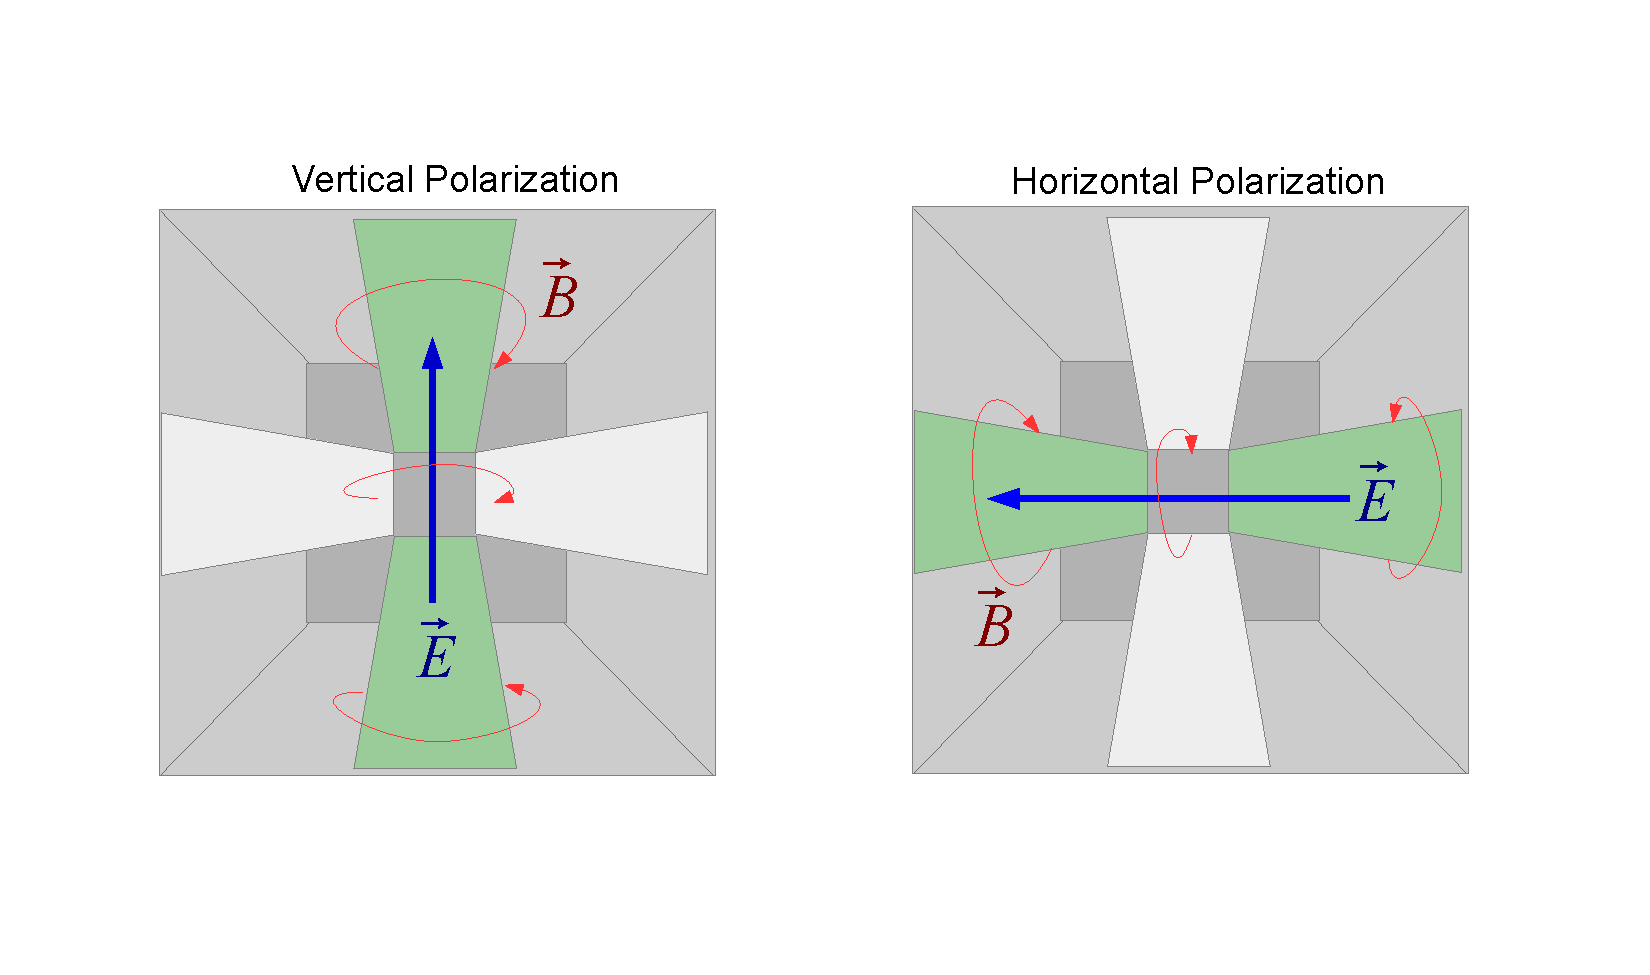
\includegraphics[width=\textwidth]{figures/AntennaPol}
	\caption{A diagram of the field line components for the Seavey dual polarization broad band horn antennas.  The E field is the principle measurement for each polarization, while the B field is the incidental cross-polarized measurement.  The antennas are specifically designed to minimize cross-polarized signal acceptance.}
	\label{fig:AntennaPol}
\end{figure}

	
	
	Calibrations of the antennas was performed over a wide range of angles in multiple configurations in order to determine the full beam-pattern of the horns in both the E-field and B-field for each polarization. See Figure \ref{fig:AntennaPol} for relation between the physical antenna and measured field orientation.  These measurements were taken for the boresight of every antenna in order to determine stability of the manufacturing process.  These measurements and variations are discussed later in the Calibration chapter.
	
%	\subsection{Antenna Theory} %seems unnecessary here?  Maybe in calibration
%		An antenna is a physical object that couples the impedance of free space to that of a a coaxial transmission wire, thus effectively converting an electric field present in a medium into a voltage that can be measured.  The principle figure of interest is in this case the antenna height, which is a mathematical construct that describes the efficiency of an antenna coupling an incident electromagnetic field into a voltage on a wire.  

	\subsection{Antenna Response Angle Justification}
		The ANITA instrument can utilize its geometric symmetry and full azimuthal coverage to reduce the response angle of the antennas and subsequently improve their signal response while keeping their noise power constant.  ANITA is very much limited by thermal background noise created from the 250K surface of the Antarctic continent, the 3K CMB, added electronic amplifier noise, and randomly placed possibly unknown anthropogenic sources.  Assuming a constant efficiency, an increase in the directivity of an antenna is linearly related to its gain by equation \ref{eqn:antGain}, where G is the antenna gain, $E_{antenna}$ is the efficiency and D is the directivity.
		
\begin{equation}
	\label{eqn:antGain}
	G = E_{antenna} * D
\end{equation}
		
		There are two maximum directivity constraints for both polarizations that each antenna must satisfy.  First, each phi sector's response must overlap with neighboring phi sector pairs to establish azimuthal directionality from interferometric baselines. Second, their elevation must encompass both up-going reflected cosmic ray and neutrino signals, as well as have some sensitivity to earth-skimming and slight down-going air showers.  As each phi sector is $22.5^{circ}$ separated from its nearest neighbor, a $30^{/circ}$ opening angle allows each sector to cover slightly over half the field of view of its neighbor.  The simple desire to have each antenna gain symmetrical in vertical and horizontal polarization then leads to a symmetric opening angle for both ridges.   Additionally, the antennas are pointed at a $10^{/circ}$ downward angle to put their maximum directivity pointed slightly below the horizon of the Earth where signals are most likely to appear.  
	
	\subsection{ANITA Low Frequency Antenna (ALFA)}
		In addition to the quad ridge horn antennas, ANITA3 flew with an additional VHF deployable "quad-slot" antenna with an omni-directional azimuthal response mounted underneath the main structure(see Figure \ref{fig:ALFA} and \ref{fig:ALFA_pic}).  As many radio frequency EAS experimental measurements are done at lower frequencies, this antenna was added to allow direct comparison between ANITA's observed particle track radiation events and those at ground based observatories.  Due to a lack of additional digitization channels in the system, as well as on-board high-pass analog filtering on the SURF board, this antenna was heterodyned with a 900MHz Local Oscillator (LO) to up-convert the signal to a measurable frequency before being combined with channel 05TH.  05TH in turn was low-pass filtered to remove it's signal and noise contribution in this signal region.  This non-symmetry in the system must be remembered in all analysis steps, and is discussed further in the Calibration section.
		
\begin{figure}
\centering
	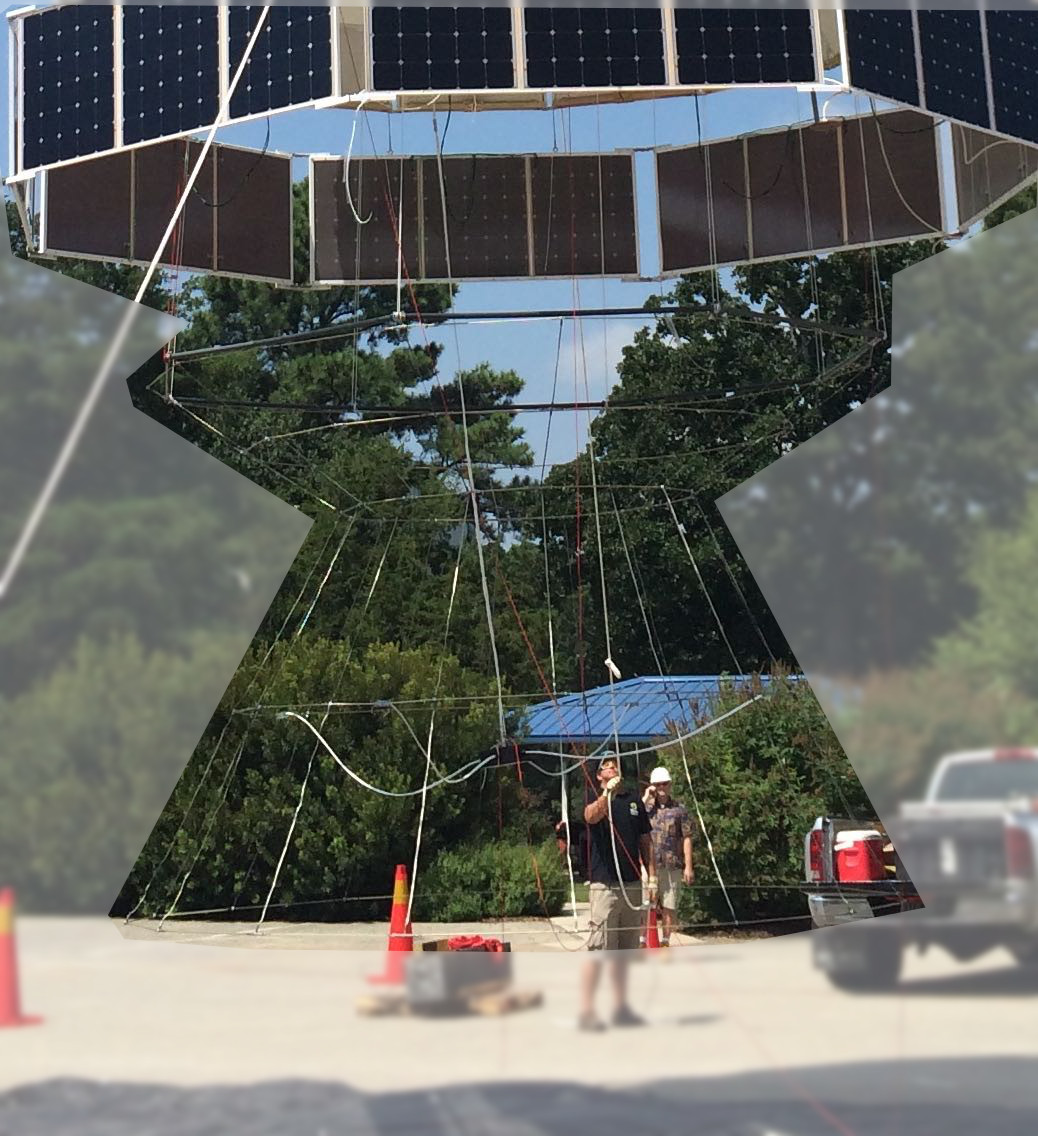
\includegraphics[width=\textwidth]{figures/ALFA_pic}
	\caption{Photo of the deployed ALFA antenna in the 2014 hang test of ANITA3 in Palestine Texas.  The photo has been edited to emphasize the outline of the antenna.}
	\label{fig:ALFA_pic}
\end{figure}

\begin{figure}
\centering
	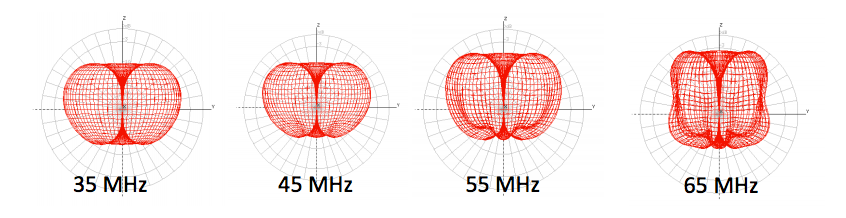
\includegraphics[width=\textwidth]{figures/ALFA_gainPattern}
	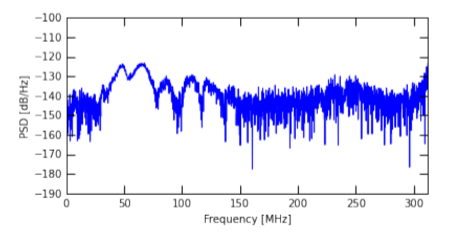
\includegraphics[width=\textwidth]{figures/ALFA_gain}
	\caption{Top: Simulations of the expected antenna gain pattern for the ALFA antenna.  Image provided by Andres Romero-Wolf.  Bottom: Measured in flight frequency response of the ALFA antenna.  Image provided by Stephanie Wissel}
	\label{fig:ALFA}
\end{figure}

	
\section{Filtering}
	\subsection{Importance}
		The radiative Askaryan and geomagnetic signal from an EAS has a very wide bandwidth, however there are a few considerations that require the signals read by the ANITA telescope be limited to a specified bandwidth.
		
		At the high frequency end of the spectrum, above 1.2GHz, the individual radiative particles in the shower core begin to be resolved, resulting in a loss of coherence of radiated power above that band (See Figure \ref{fig:AskaryanSimulation}.  This effect is stronger at angles further from the peak Cherenkov angle away from the shower axis.\cite{PhysRevD.84.103003}  This lack of coherent signal power in the UHF region provides a high frequency suppression to the total signal bandwidth.

		On the low frequency end of the spectrum, the radiated power from the shower is expected to rise as a function of frequency up to 1GHz.  Manufacturing and design limitations of a long wavelength antenna coupled with the high utilization of the VHF band by radio transmitters on satellites and ground stations lead to a requirement that lower frequencies, below 180MHz in the case of ANITA3, be removed.
		
	\subsection{Technical Details}
		This band pass filtering is done in two stages, one immediately after the antenna, before the pre-amplifier in order to prevent saturation of the pre-amplifier from out of band signals, and one after the amplification chain in order to remove out of band amplifier noise.  The primary filter must have an extremely low in-band loss, as any loss introduced by the filter is gained in full system noise temperature, a value which is cascaded through the entire amplification chain.  This was accomplished with a custom made LARK band pass filter.  The secondary filtering was accomplished with two discrete low-pass/high-pass filters that do not require such a low in band loss characteristic due to their position in the signal chain.
		
	\subsection{Digitizer Bandwidth}
		The LABRADOR digitizer also influences the selection of the band edges.  The maximum sampling rate of 2.6GS/s yields a 1.3GHz nyquist sampling frequency utilyzing .  Any out of band power will be aliased into the signal band and present itself as increased in-band noise.  Additionally, the 100ns SCA buffer length would only allow a minimum 10MHz full period oscillation to be observed.  However in reality the major limitation at lower frequencies remains to be the antennas.  The effect of the limited trigger window is visible in the ALFA low frequency antenna, as much of the 
		
\section{Amplification}
	Expected signal strength output from the coupling of the antennas to the 50-ohm RF transmission network requires that signal amplification occurs to be detectible by the available electronic instruments.  The amplification for the ANITA3 instrument was accomplished with two stages, one close to the antenna within the custom built module, and one upon entering the instrument crate itself within the iRFCM (internal radio frequency conditioning module).  
	
	\subsection{First Stage Amplifier: The AMPA and DDAMPA}
		The front end amplification was accomplished by two similar custom built modules named the Antenna Mounted Pre-Amplifier (AMPA) and the (historically named) Drop Down AMPA (DDAMPA).  Depicted in Figure \ref{fig:AMPAandDDAMPA}, each enclosure contains components for filtering, amplification, and a bias network power trasmission component.  
		
		
\begin{figure}
\centering
	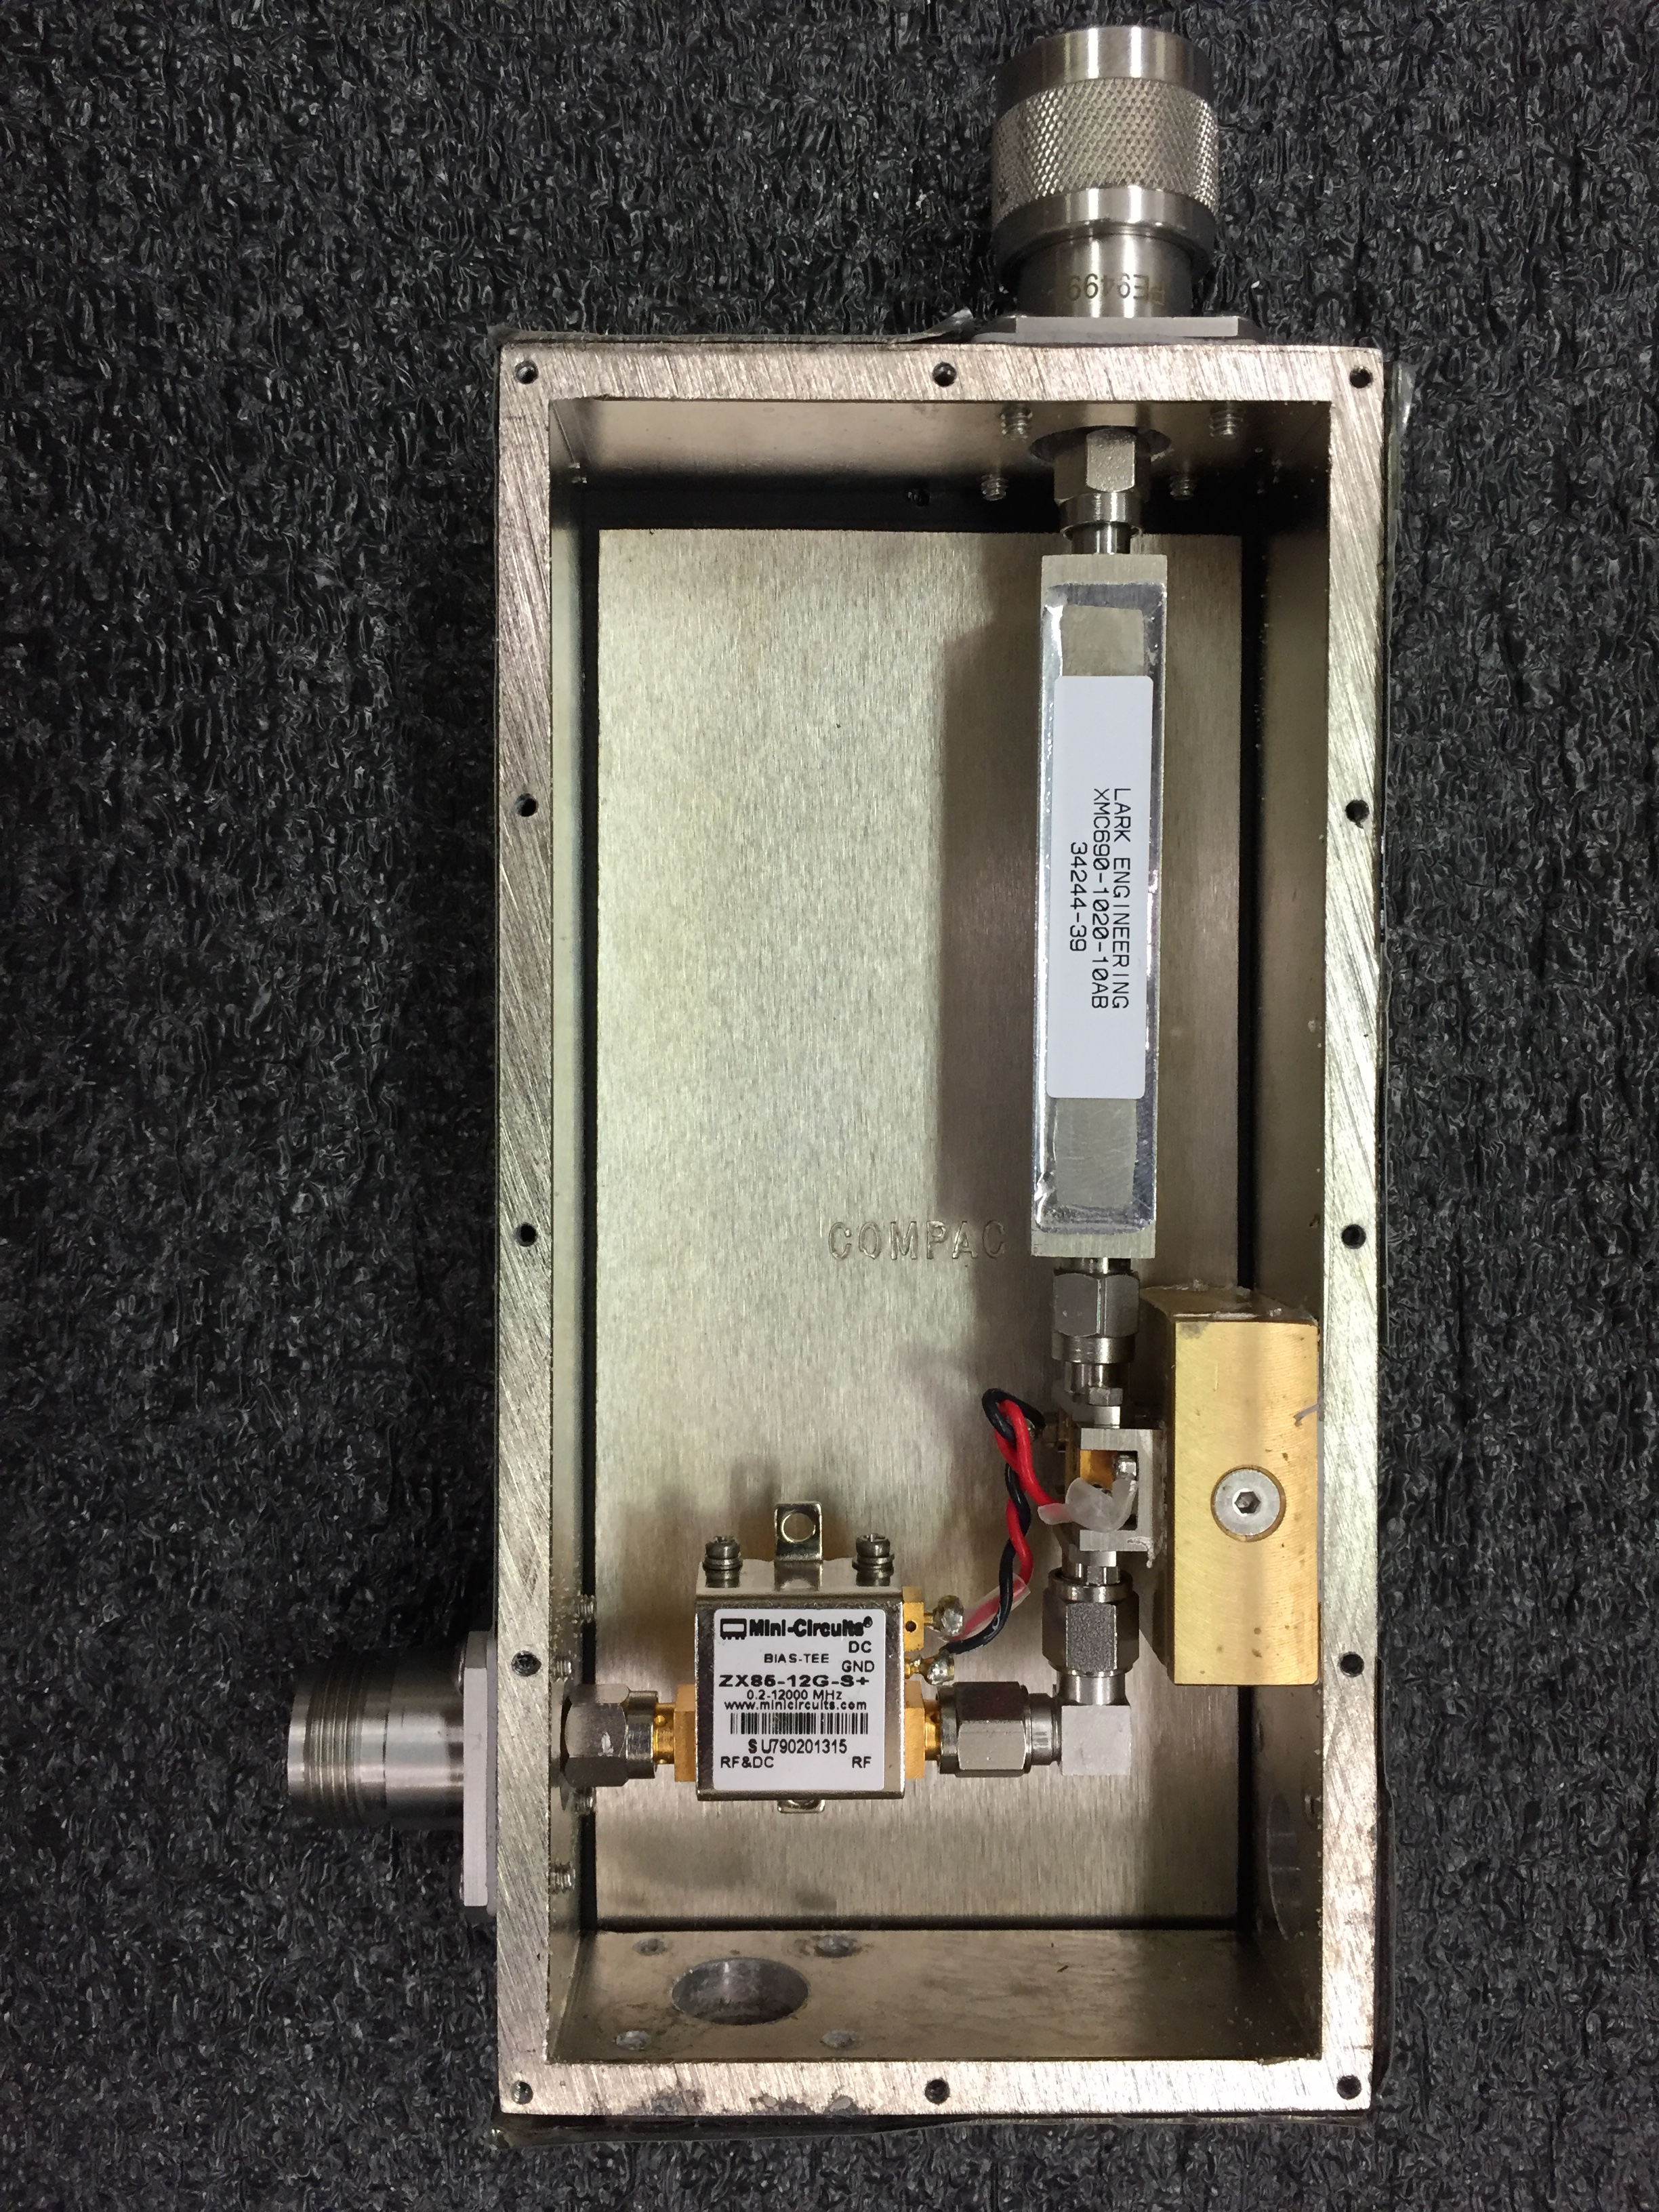
\includegraphics[width=0.45\textwidth]{figures/AMPA}
	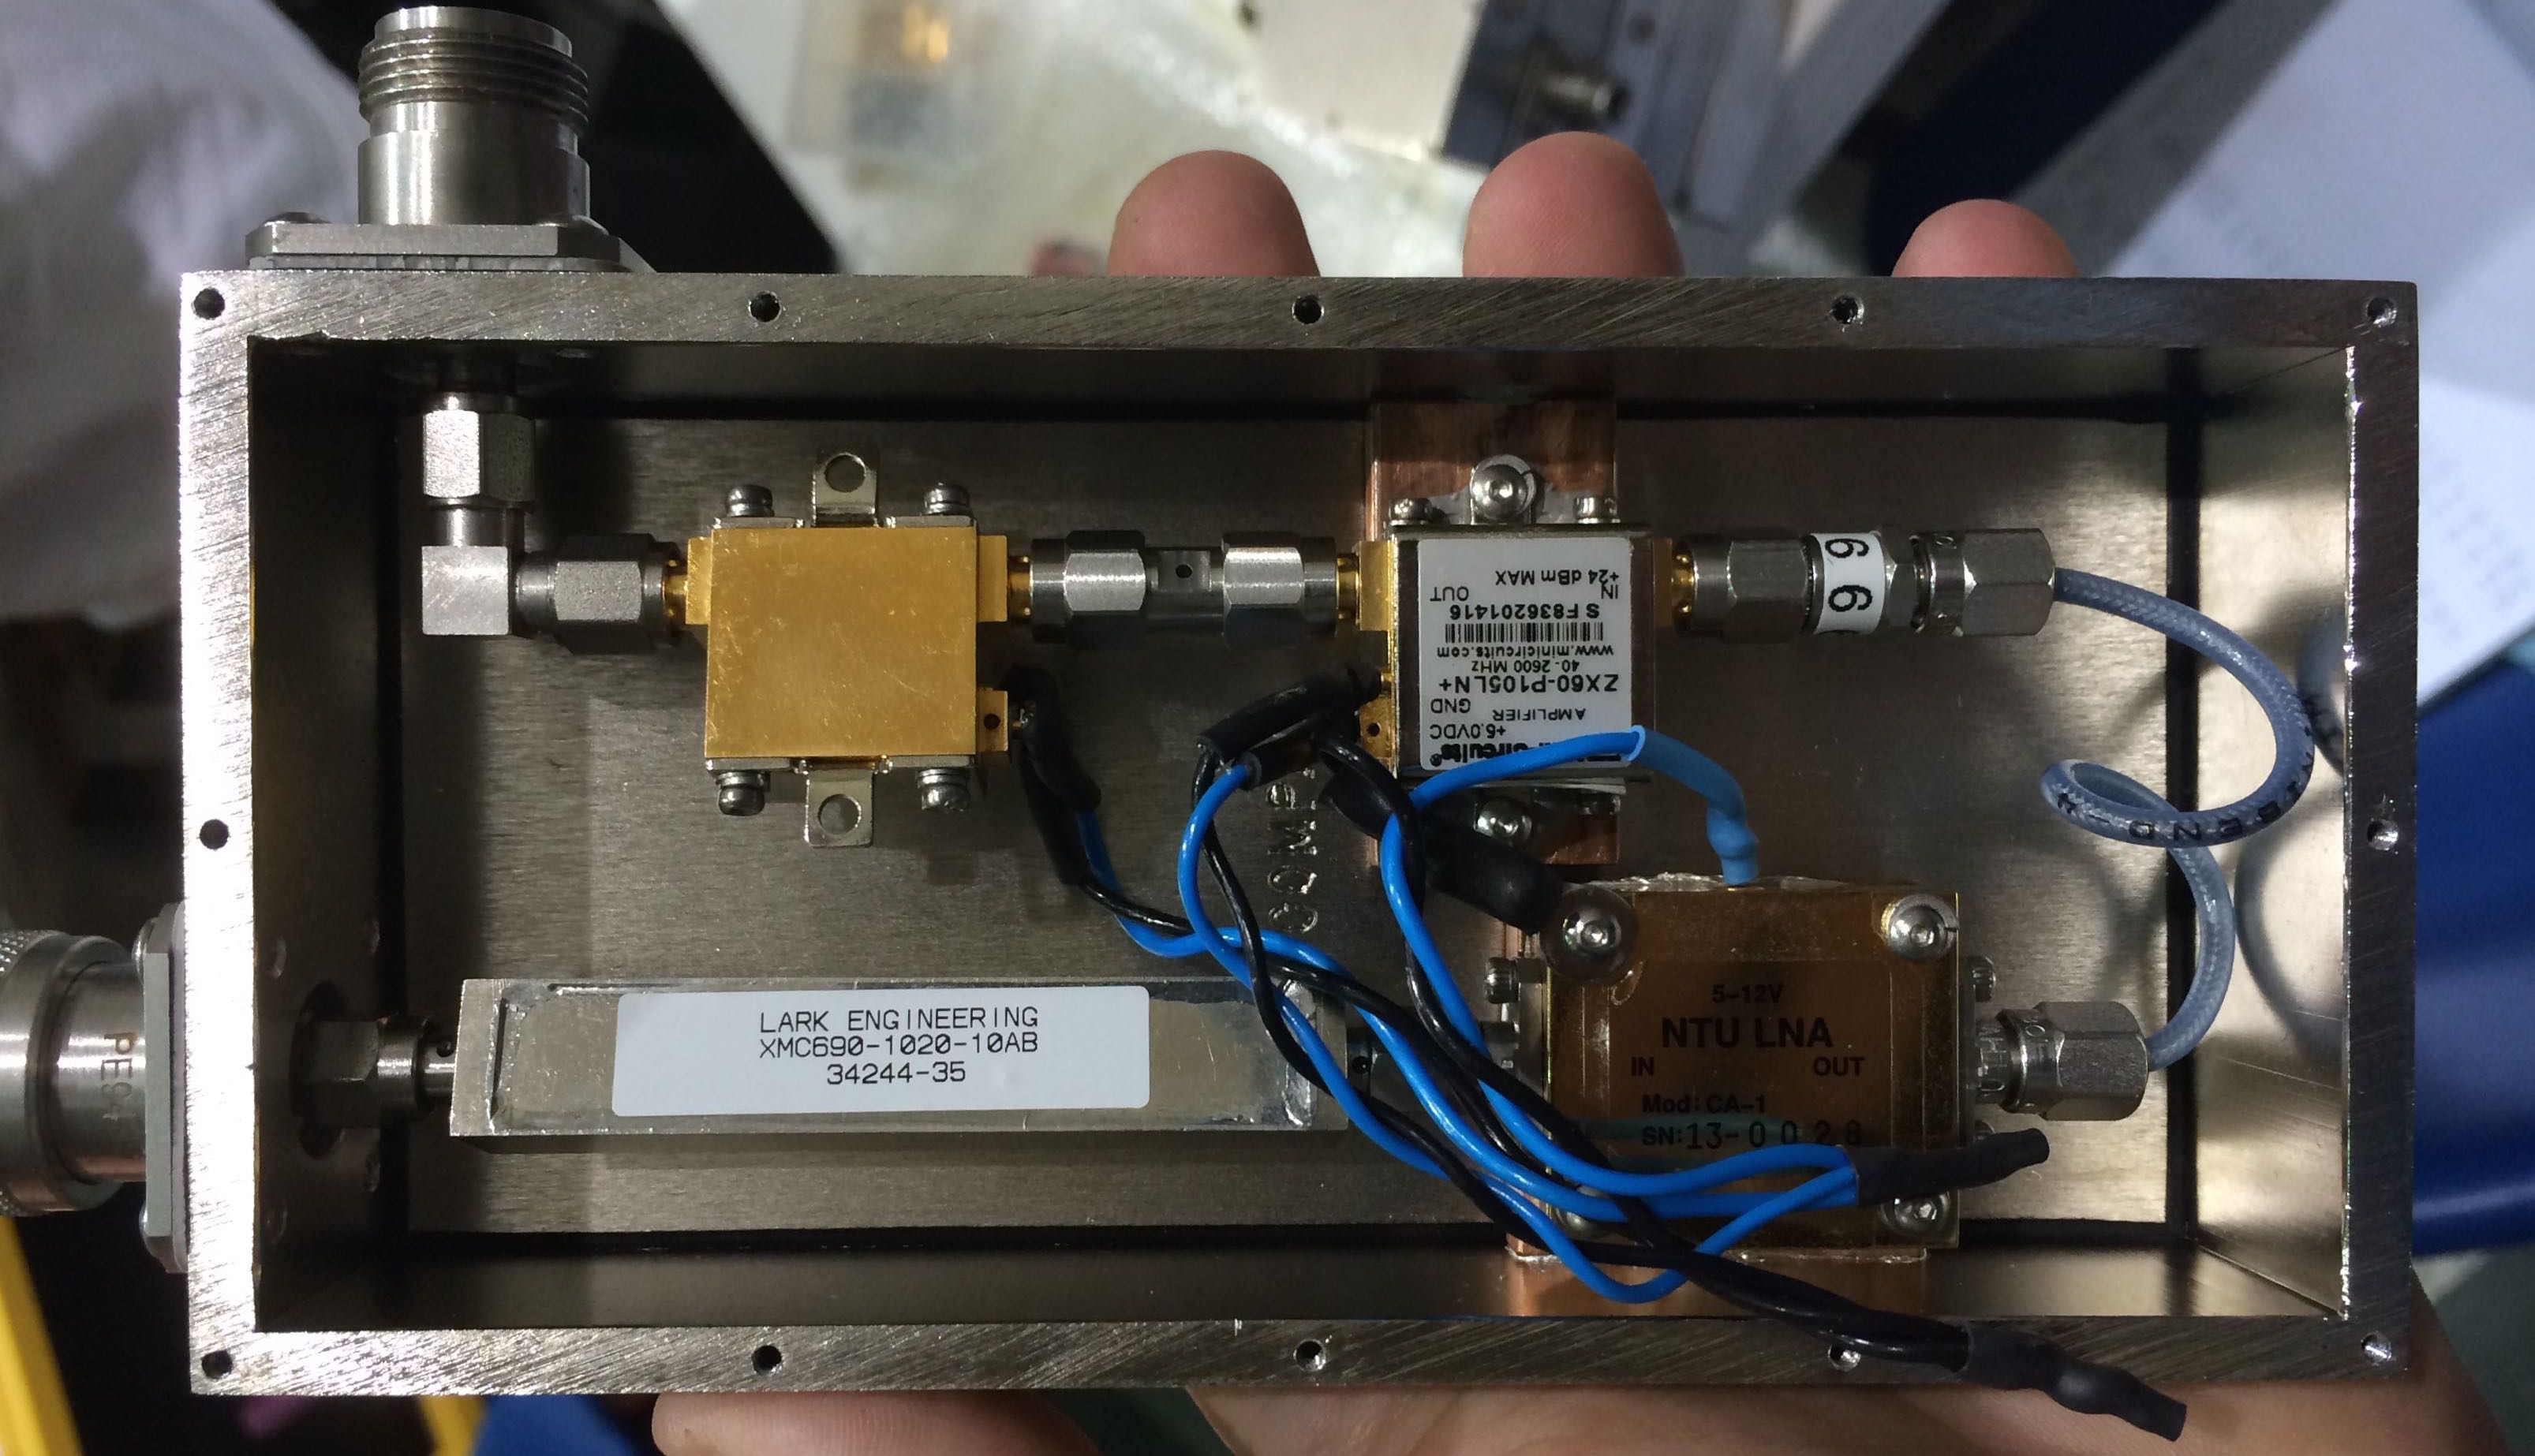
\includegraphics[width=0.45\textwidth]{figures/DDAMPA}	
	\caption{The AMPA (left) and DDAMPA (right) internals.  Thanks to Jarred Roberts for AMPA picture}
	\label{fig:AMPAandDDAMPA}
\end{figure}	

\begin{figure}
\centering
	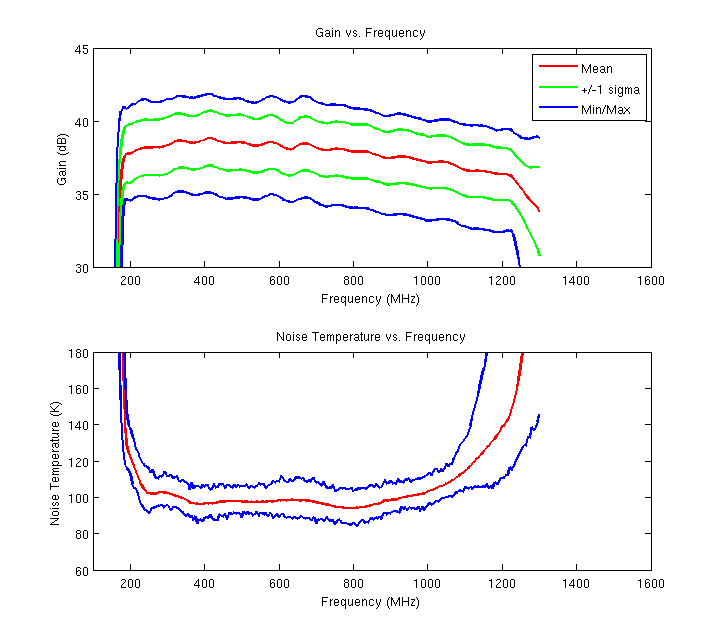
\includegraphics[height=0.45\textheight]{figures/ampas_std}
	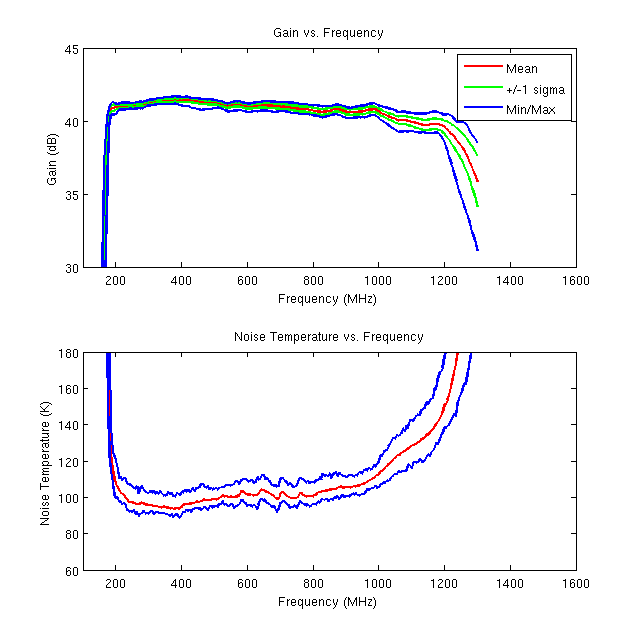
\includegraphics[height=0.45\textheight]{figures/ddampas_std}	
	\caption{Mean and standard deviation of gain and noise figure measurements for the AMPA (top) and DDAMPA (bottom) amplifier modules.  From Elog 560}
	\label{fig:AMPAandDDAMPA_std}
\end{figure}	
	
	\subsection{iRFCM}
	The four custom built iRFCM enclosures, one of which can be seen in figure \ref{fig:IRFCMpic} and is described in \ref{fig:IRFCM}, handle the second stage amplification for twenty four of the RF signal channels.  There are three major active RF components for each signal chain present within the module. The AmpLite, a high gain, high dynamic range amplifier built by Patrick Allison of OSU, a tuning attenuator for gain balancing of the 96 different channels, and a bias-tee which, as its name suggests, adds a DC bias to the center conductor of the coaxial transmission cable between the AMPA and the iRFCM.  This bias is used to power the AMPA and DDAMPA amplifier modules.

	
\begin{figure}
\centering
	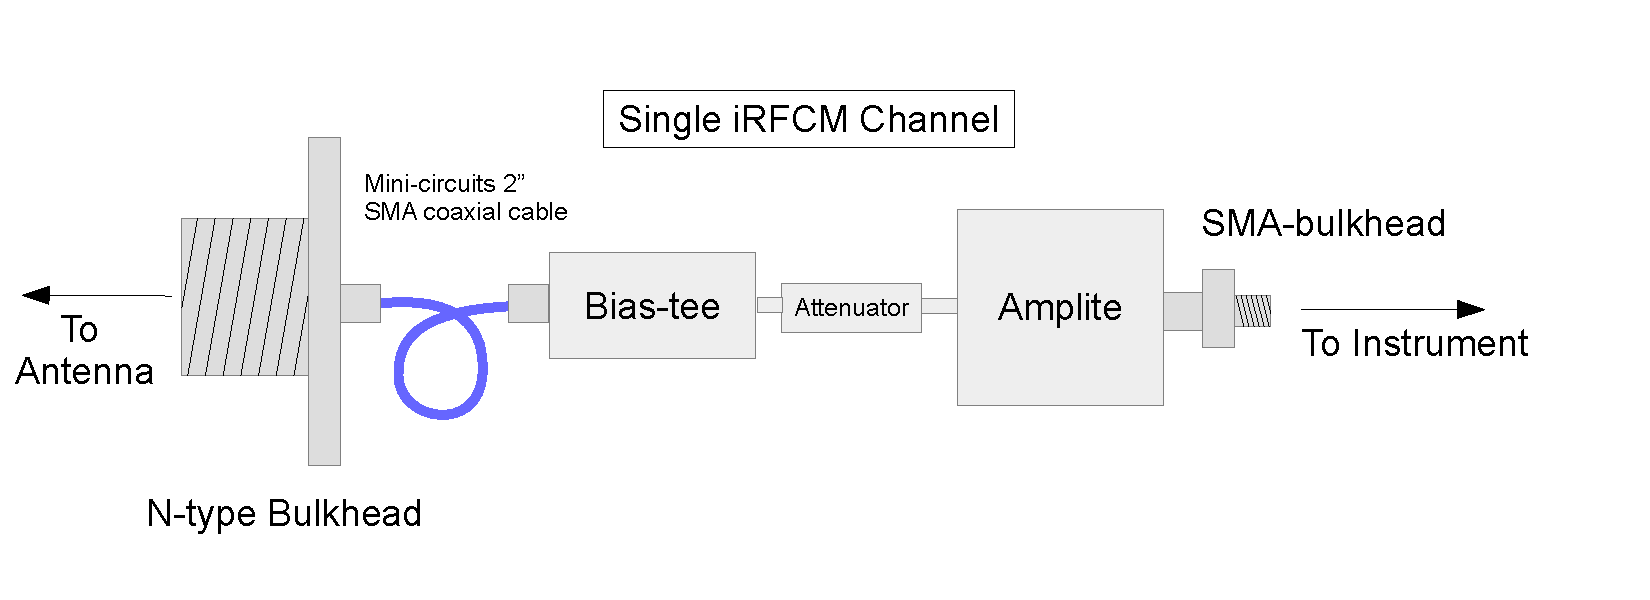
\includegraphics[width=\textwidth]{figures/IRFCM}
	\caption{A block diagram of a single iRFCM RF channel.  The bias-tee, as its name suggests, adds a DC bias to the signal }
	\label{fig:IRFCM}
\end{figure}
	
	
\begin{figure}
\centering
	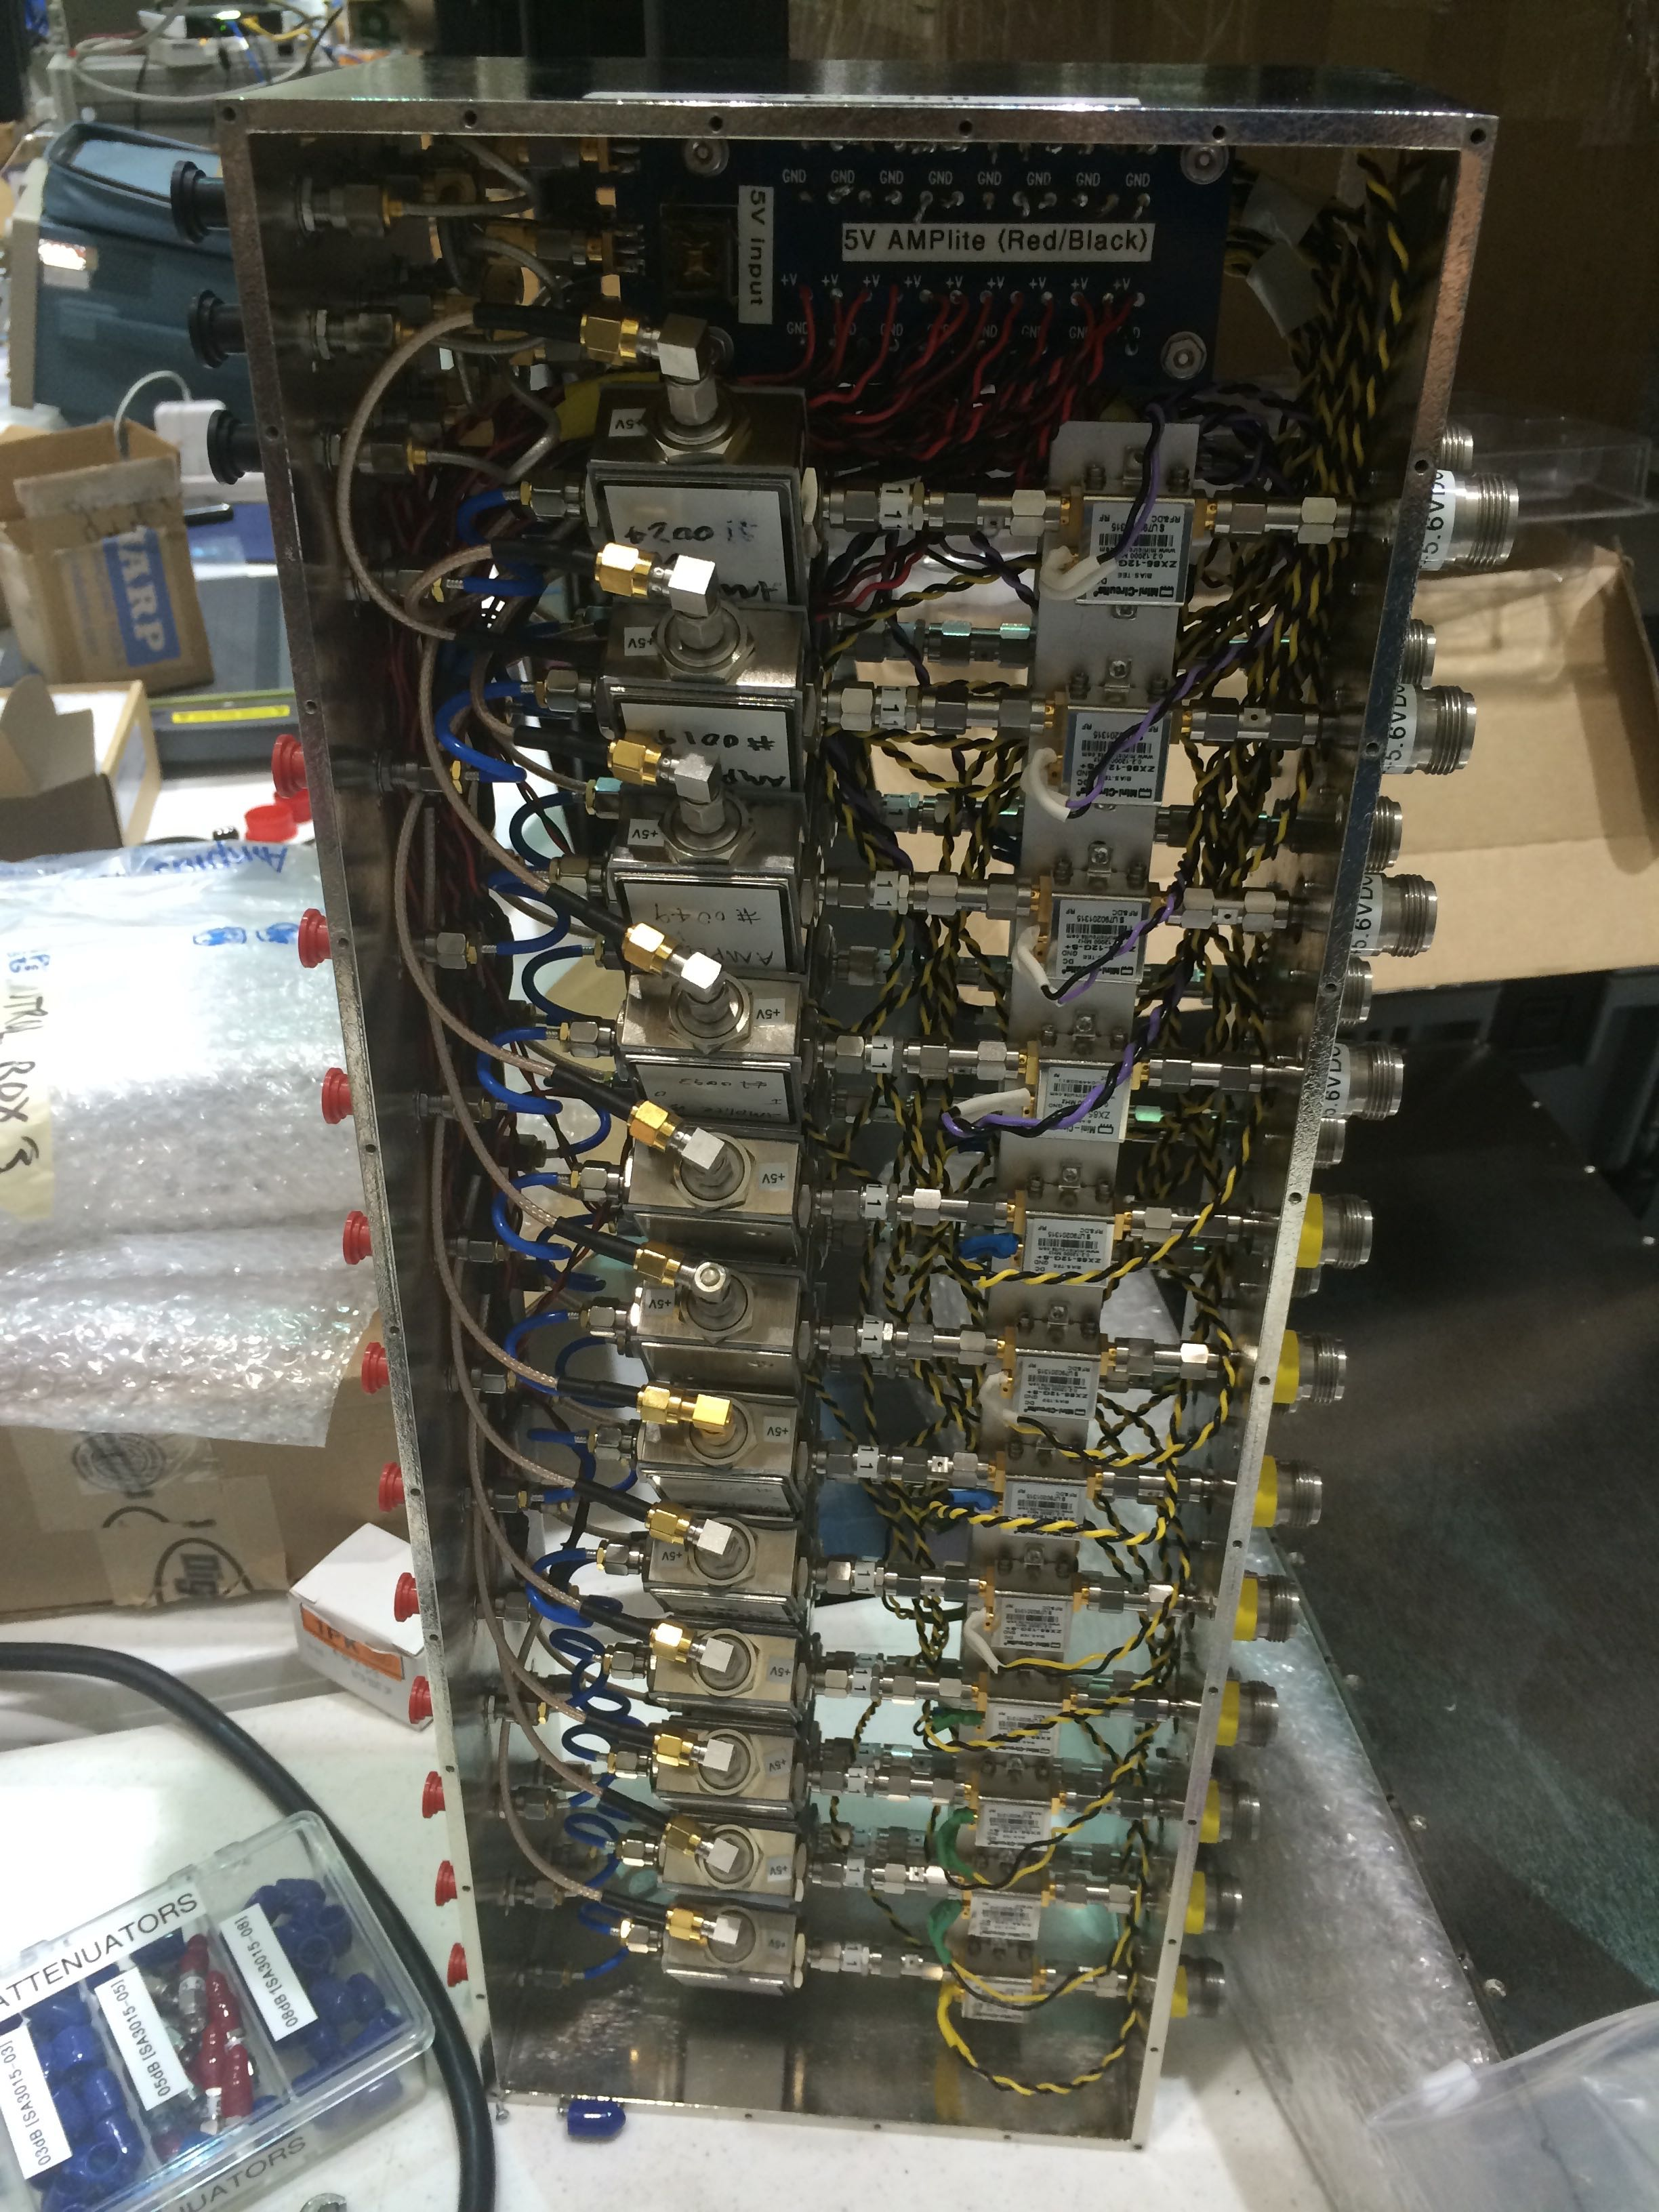
\includegraphics[height=0.9\textheight]{figures/IRFCMpic}
	\caption{An image of the internals of an iRFCM module after assembly}
	\label{fig:IRFCMpic}
\end{figure}
	
	
	\subsection{Expected electromagnetic field variations}
		Depending on the radiation mechanism being observed, the power of an EAS signal measurable at the detector is proportional to the energy of the incident cosmic ray particle.\cite{EASSignalPower}  This signal power is superimposed on the thermal and anthropogenic background noise present in the field of view of the detector.  The constant thermal emission of matter in the field of view of an antenna introduces a Johnson-Nyquist thermal noise component, which is calculated in Equation \ref{eqn:NyquistNoise}

\begin{equation}
	\label{eqn:NyquistNoise}
	P = k_{b}T\delta F
\end{equation}

Where P is the thermal noise power observed across a termination resistor in watts, $k_{b}$ is Boltzmanns constant, T is the absolute temperature observed temperature in kelvin, and $\delta F$ is the frequency bandwidth in Hz.  The antenna, creating a smooth transition between the complex impedance of free space and that of the coaxial transmission network, has a noise temperature dictated by the integral of the temperature of objects in its field of view $(T(\theta,\phi))$, weighted by the gain pattern of the antenna $(G(\theta,\phi,\omega))$, shown in equation \ref{eqn:antTemp}.

\begin{equation}
	\label{eqn:antTemp}
	\int_{-\pi}^{\pi}\int_{\theta}^{2\pi}\int_{0}^{\infty} G(\theta,\phi,\omega)*T(\theta,\phi)sin^{2}\theta d\theta d\phi d\omega
\end{equation}


	\subsection{Noise Figure} 
	The requirement of amplifier chains leads to a minimum of additional electronics noise introduced by the detector.  Besides a background of thermal noise, the dominant continuous noise source is electronics noise from the amplifiers.  This noise is a byproduct of the non-ideal coupling of the amplifier to the input signal that results in the amplification of internal thermal noise seen as a resistance on the front of the amplifier.   This noise, unlike the thermal noise incident on co-pointing antennas, is not coherent as each amplifier adds its own uncorrelated noise component.  The noise figure is additionally increased by any loss of power in front of the amplifiers.  Since the noise figure cascades through an amplifier chain, it is imperative to reduce any additional noise figure at the beginning of the signal chain, and less important in the subsequent amplifiers.  The cascading noise can be calculated using Frii's Formula (Equation \ref{eqn:noiseCascade}), where $T_{total}$ is the resulting noise temperature of the entire signal chain, $T_{n}$ is the noise temperature of a specific element, and $G_{n}$ is the gain magnitude of a specific element.
	
\begin{equation}
	\label{eqn:noiseCascade}
	T_{total} = T_{1} + \frac{T_{2}}{G_{1}} + \frac{T_{3}}{G_{1}G_{2}} + ... + \frac{T_{n}}{G_{1}G_{2}...G_{n-1}}
\end{equation}
	
	From this, one can see that the +38dB of gain from the first stage amplifier reduces any subsequent noise figure from components by a factor of $38dB = 10*log(G) \rightarrow 10^{38/10} =  6309 = G$. alleviating the requirement for low noise amplifiers in subsequent stages.


	\subsection{Dynamic Range}
		The absolute power level of the signal travelling through the system is dependent on the end-of-chain termination and instrumental device, and must be tuned appropriately.  For example, the digitizer ASIC can cover a 2.5V full dynamic range.  An observed voltage with peak amplitude significantly below that level would never exercise the range boundaries of the digitizer.  A negative drawback to this wasted range is that the lesser significance bits lose sensitivity to low voltage oscillations, as fewer total levels fully encompass the full signal.  Equally and oppositely, too high an input power signal would become distorted at high peak amplitudes. Other systems at termination ends of the branching signal chain have similar dynamic range limitations and must be tuned appropriately.
		
		
	\subsection{Gain Justification}
		The required gain of the system can be arrived at by determining the maximum terminal instrumentation requirement input power, then calculating what additional amplification is required to meet that specification.  Any terminal instruments that require lower input power are achieved by in-line, flat spectrum, fixed attenuator components.  \ref{tab:rfLinkBudget} is a table of the terminal components, their dynamic ranges, and the required gain necessary to put observed thermal noise from the antenna into a measurable power region.  Components not yet mentioned in this thesis are covered in subsequent sections in this chapter.
	
\begin{figure}
	\centering
	\label{tab:rfLinkBudget}
	\begin{tabular}{| l | c | c |}
		\hline
		Component & Dynamic Range & Gain Requirement\\
		\hline
		LABRADOR digitizer & 20dBm & 80dB \\
		RF Power Monitor & -10dBm & 50dB \\
		SHORT Tunnel Diode & 0dBm & 60dB \\
		\hline
	\end{tabular}
	\caption{A description of the required input power and gain requirements for the three terminal instrumentation components of the ANITA3 system}
\end{figure}
	
	
\section{Digitization}
	The electric field variations incident as a function of time is digitized using an array of fast analog to digital converters (ADCs), custom designed application specific integrated circuits (ASICs).  The ANITA3 instrument utilizes a LABRADOR (Large Analog Bandwidth Recorded And Digital Ordered Readout) chip, designed by Gary Varner.  It is a 12-bit, 2.4GS/s, 256 sample long ADC, yielding a window size of ~100ns.  This is accomplished with a sample and hold ring buffer read out with a wilkinson clock comparing the stored charge in a storage capacitor against a ramp signal driven by a constant current source.  Each chip receives 8 RF analog inputs, as well as a 9th clock channel coincidently propagated to all LAB chips.  The SURF (Signal Unit for Radio Frequency) Board consists of 4 LABRADOR chips in order to create a buffer for continuous sampling.  

	\subsection{LABRADOR3 ASIC}
		The third iteration of the Large Analog Bandwidth Recorder And Digitizer with Ordered Readout (LABRADOR, or LAB3) has been in use on ANITA flights due to its extremely low power and high precision.  It consists of a nine RF channels fed into separate 260 cell capacitor ring buffer and can operate at sampling frequencies of 2.6GS/s, or a Nyquist limit of 1.3GHz.  In addition, it has a large dynamic range and a gigahertz of bandwidth in the UHF spectrum.  The sampling time base is driven by a phase inverting Ripple Carry Out pulse that propagates internally to the chip.  The continuous sampling is halted when a trigger is issued to the chip, and a Wilkinson Clock measuring the Time To Threshold of a constant current ramp voltage converts the stored charge in each capacitor to a digital value that is read out in parallel to an FPGA for storage.  Due to the dead time related to the digitization process, four LAB3 chips are placed in parallel in order to ensure continuous sampling even when a single LAB3 is reading out its values.  When a hold is issued, the LAB3 chip returns both an estimate of which RCO phase it is in (which is incorrect near the wraparound region), as well as the locations of the "HitBus", or samples that are currently connected to the RF input. The procedure and results of calibrating this readout is detailed in the Calibration section.
		
\begin{figure}
\centering
	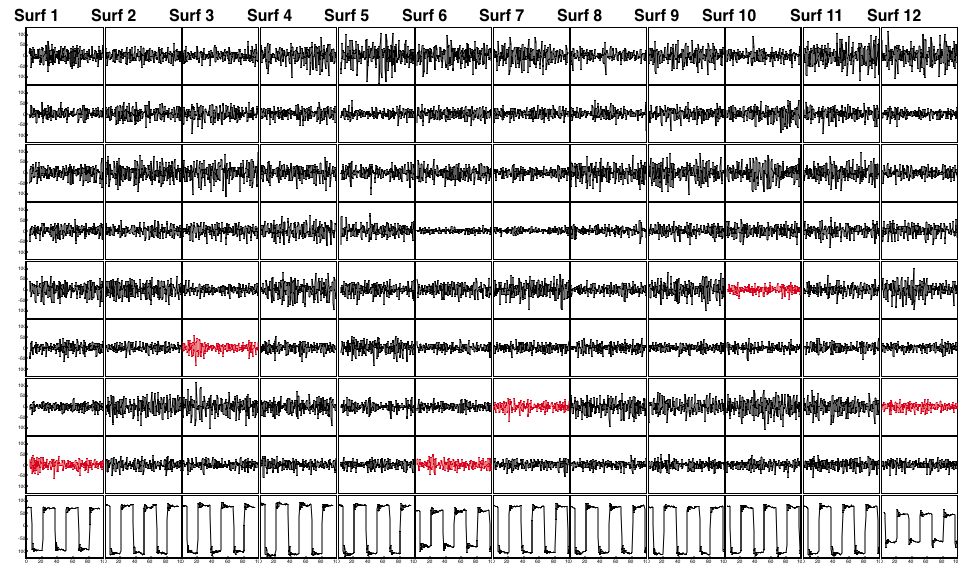
\includegraphics[width=\textwidth]{figures/waveformSnapshot}
	\caption{An example readout of all 96 channels of the full ANITA3 detector, organized by SURF (columns) and channels (rows).  Bottom row is the synchronization clock inserted into all LAB chips.  In red are phi sectors that triggered the event.  This particular waveform is low SNR self triggered WAIS calibration pulser (ev 61326092).  Image made with MagicDisplay data visualization code.}
	\label{fig:waveformSnapshot}
\end{figure}
		
	
	
	\subsection{Limitations}
	After a hold is issued to a chip, the digitization freezes the ring buffer and yields the chip unable to sample until readout is complete, a process that can take ~1us.  During a readout, no new data can be captured by the LABRADOR chip.  To alleviate this, the RF input chain is separated into four separate chips which are read out one at a time.  This provides a buffer depth of four which allows the instrument to remain live even while reading out several repetitive events.
	
	The analog bandwidth of the LAB3B (used in the ANITA3 and ANITA2 experiments) did not fully cover the full bandwidth of the antennas and signal chain due to coupling into the chip through the bond wires in the package.  This yields a drop-off in sensitivity to high frequency signals.  
	
	The time between samples is controlled by a charge starved transistor chain that controls the connection between the sampling capacitor and the input RF signal.  Due to process inconsistencies in the manufacturing of the ASICs, the timing between subsequent samples is not well controlled.  This yields a variable delta T that needs to be corrected in calibration of each chip individually.  In addition, it leads to an unevenly sampled time domain waveform, which introduces a difficult to correct frequency response, and requires interpolation between points before creating interferometric maps.  This is processing intensive, an issue that makes doing on board interferometry more difficult.
	
 	Since each LAB chip can only digitize eight channels concurrently, a total of twelve total SURF boards are required to read out any particular event simultaneously.  The dispersal of the readout HOLD signal from the FPGA, and its subsequent latching on each LAB, adds jitter that needs to be corrected out.  The ninth channel on each lab observes a 33.3MHz analog clock signal propagated through the CPCI backplane to each SURF.  By measuring the relative phase of this clock between SURFs, a correction for this jitter can be done.  This is discussed further in the Calibration section.
	
	\subsection{Impulse Response}
	The filtering and amplification chain has a dispersive effect on the signal, which requires a calibration of the system impulse response in order to fully understand the incident electromagnetic field.  An impulse response is the phase and gain distortion created by the RF network to an input signal.  In the ANITA system, an band limited case, the phase shift increases as a function of frequency, which causes the signal power to be temporally spread.  As a cross-correlation between multiple channels is dependent on the full complex parameters of the signal, significant variation between the impulse responses of channels will result in a reduced maximum correlation value regardless of the electromagnetic impulse present at the antennas.  The ANITA instrument is designed to be identical and symmetrical across all 96 channels, making this effect small and constant.  Measurements of this response and calibration are done in the Calibration section, and the effect and deconvolution is detailed in the Analysis section.

	
	\subsection{Future development}
	Since the LAB3B was developed in 2005, there has been significant development in the LABRADOR architecture.  The most modern generation of chip, the LAB4D, is a single channel readout that improves upon the previous generations by both vastly increasing the storage buffer through use of a Storage Capacitor Array (SCA) to increase the record length or buffer depth of the chip.  It also allows for the correction of dT offsets iteratively onboard the chip, minimizing the requirement for post-digitization correction of the waveform and the subsequent high-frequency signal loss.  The quantitative effects created from a large dT variance are discussed later in this thesis.
	
		
\section{Triggering}
	As the time domain digitization window is extremely small (100ns is one ten millionth (1e-7) of a second) and ANITA is limited to a 50Hz readout rate, it is necessary to selectively trigger on segments of time that have a high probability of containing a signal event.  The physics signal created by a UHE particle interaction within the field of view of, and directed towards, the instrument exhibits itself as a picosecond duration impulsive electrical potential emanating from a specific direction.  The background is random incoherent thermal noise or single band constant power anthropogenic sources.  As there is no digitizer buffering or analog delay lines, the triggering system must combine together information from several RF channels without full digitization and form a decision quickly, before the waveform is overwritten in the ring buffer of the LABRADOR digitizer.  For the ANITA3 system, these triggering decisions were made in the Triggering Unit for Radio Frequency (TURF), which receives trigger information for each channel from FPGA comparator electronics on each SURF through the CPCI backplane passthrough connectors.
	
	\subsection{SHORT square-law power integrator}
		A solution to triggering employed in many RF transient detector experiments is to utilize a square-law integrating power detector.  An Ezaki diode (or tunnel diode), is a nonlinear semiconductor circuit that, in a specific input power region, essentially rectifies and integrates an incoming RF signal through the quantum mechanical effect of electron tunneling.  The diode is capable of taking the extremely fast impulsive signal, with a pulse width of under 1ns, and distributes the power over a longer time scale while simultaneously increasing the signal to noise power ratio.  This allows a clocked comparator circuit, usually running with a max of 4ns/cycle, to latch a electrical signal that crosses a certain threshold.  These L1 triggers can be tuned to a reasonable rate, the specifics of which is detailed below, by altering the comparison voltage with an on board DAC, and each channel can be kept running at a similar rate with a PID loop.  Comparing the timing of these "L1" triggers between antennas with similar pointing directions allows a massive decrease in overall trigger rate dictated by combinatorics.
		
\begin{figure}
	\centering
	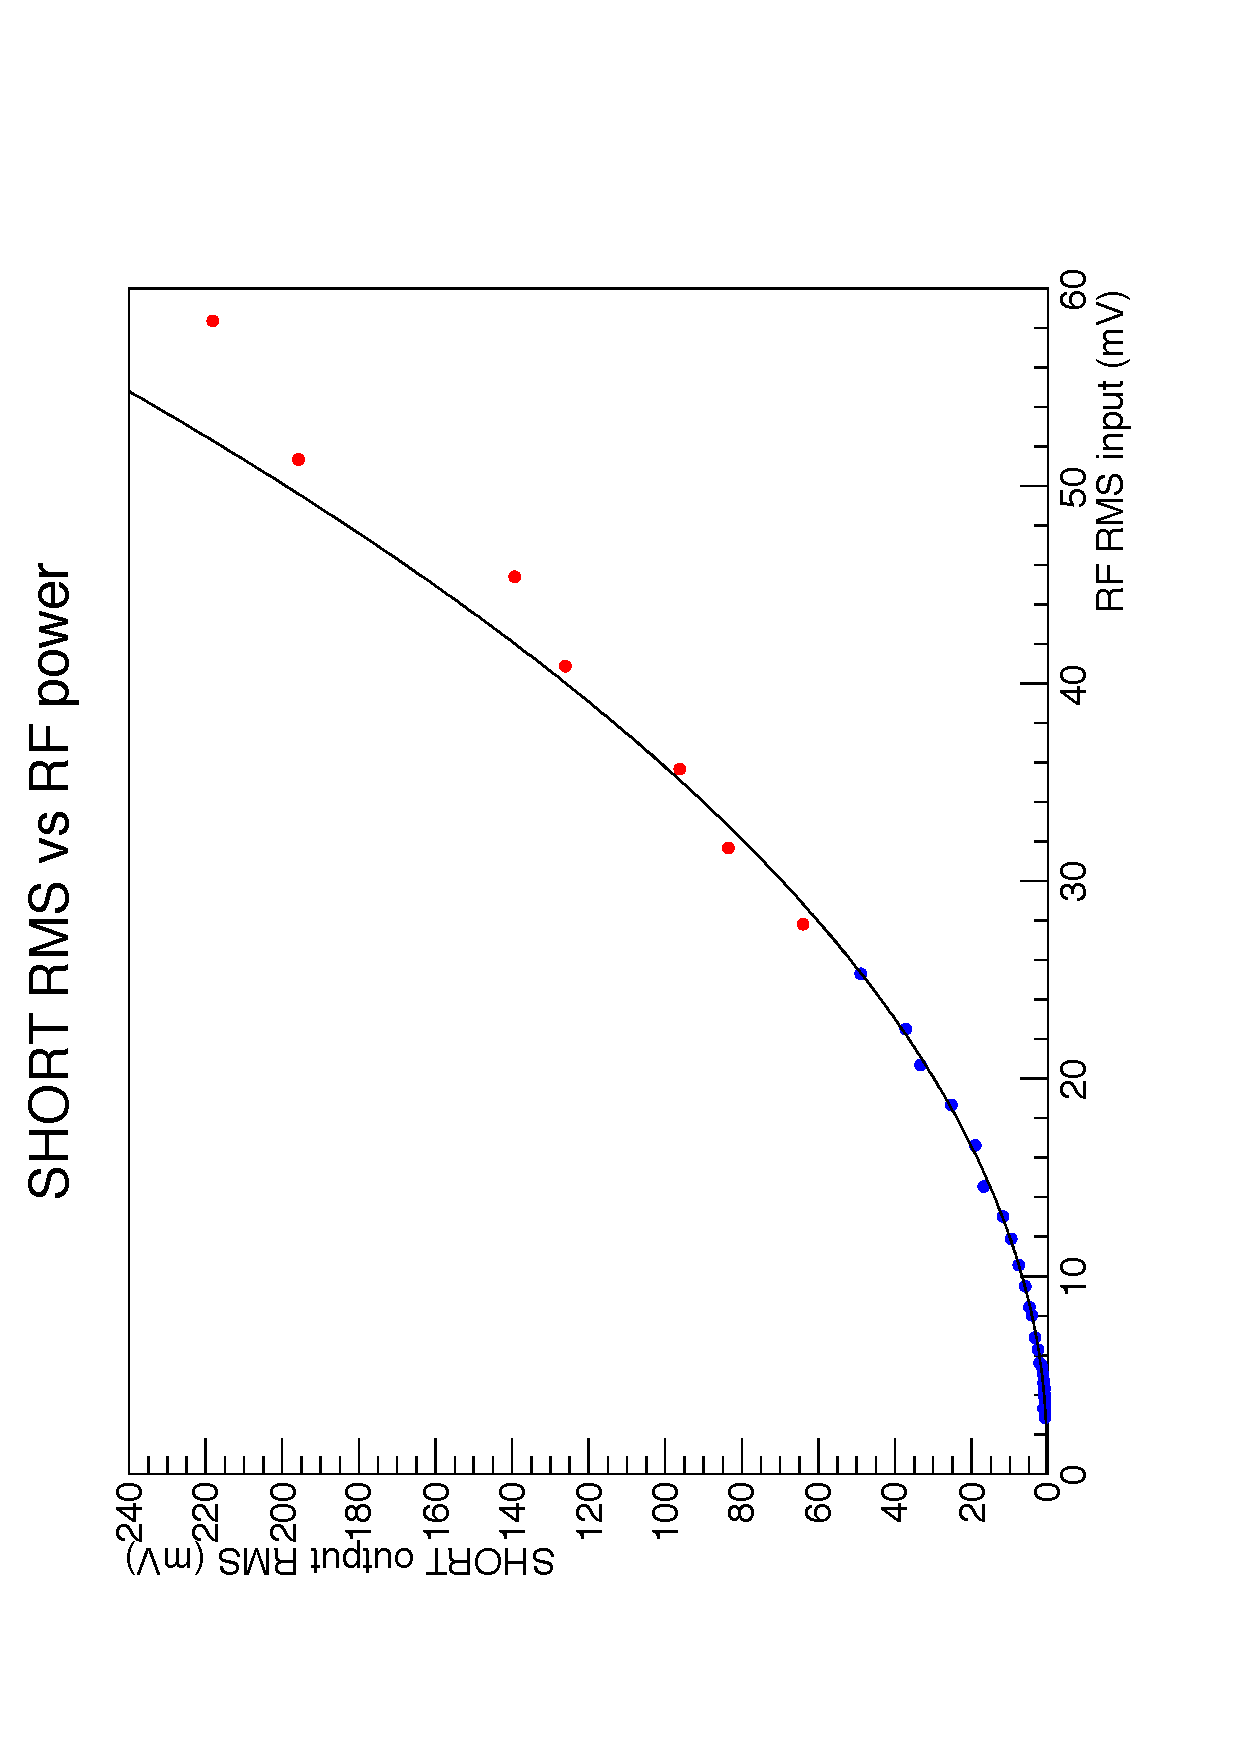
\includegraphics[height=0.8\textheight,angle=-90]{figures/RMS_in_out}
	\caption{Measurements of the response of the SHORT tunnel diode "square law" RF power detector taken in Palestine TX in 2014.  Thanks to Katie Mulrey for the plot}
	\label{fig:SHORT_square}
\end{figure}
		
	
	\subsection{Trigger Heirarchy Overview}
		The triggering system is divided into several sub-triggers that layer hierarchically to arrive at a global trigger decision.   These range from the individual power law thresholding to a time windowed combinatoric trigger between multiple channels.  In ANITA3, the trigger is split into a vertical (Vpol) and Horizontal (Hpol) trigger system, as the two differing particle shower sources (in ice neutrino interactions vs geomagnetically dominated air showers) will have mostly orthogonal polarization.  These two trigger paths are identical and have equal weighting in the final global trigger decision.  
		
		The first trigger level, or what I'll call the L0 trigger (it is also known as the L1 trigger depending at what value one begins counting), is a comparator circuit on the FPGA between the output of the SHORT and a tunable DAC. It is thus possible to tune each channel individually to give an even weighting in the ultimate trigger decision.  This is done by measuring the number of threshold crossing counts per time fraction observed by each comparator circuit, also called the scalar rate.  This scalar rate is monitored by a software PID servo loop that attempts to keep all channels equal.
		
		The secondary trigger level, or L1, is a phi sector specific time dependent windowing function that combines the L0 triggers from all three channels in a single phi sector.  A real plane wave signal incident on a phi sector will have a causal separation in time, while incidental noise threshold crossings will be uncorrelated in time.  These timing offsets are used to create a metric for discriminating on noise up to the level of precision provided by the FPGA trigger electronics.  
		
		The final trigger, or L2 is a requirement that two neighboring phi sectors decide a L1 trigger within an 8ns window.  This leads to the ultimate requirement that four out of six like-polarized antenna channels with an overlapping field of view observe a transient power fluctuation.  Additional details of each level trigger are detailed below.
		

	\subsection{L0 Tiggering efficiency and quality}
		The trigger must make a trade off between efficiency, the ratio of real signals selected for digitization over the total number of signals incident on the detector, and quality, the ratio of the number of true signal event over total selected events.  A perfect detector would have an efficiency of 1 and a quality of 1.  However in reality these values are both a function of the total maximum readout rate for the detector, which places a maximum limit on the number of events capable of being selected.  As an example, if the trigger constantly selected all moments in time it would be perfectly efficient, but the quality of the signal would be horrific.  Inversely, if the trigger was set to have perfect quality and only select extremely high power impulsive events, it would have poor efficiency for low SNR signals.  The efficiency of the detector can be statistically measured by injecting signals of varying signal to noise ratio (SNR) at a known rate and observing the rate of measured signals.  This will produce a curve (as seen in a plot I will add) which has a characteristic shape, of which the 50\% efficiency point is the defining metric.  This point will be directly related to the allowable incidental noise trigger rate, which was decided to be set at a rate where the payload would be "dead" for approximately 5\% of the time.  I have to add plots for these things!
		
	\subsection{L0 Optimization}
		What little room lies in optimizing the SHORT circuit is entirely in tuning the input power to the tunnel diode circuit.  The inverse-resistance region, where a decrease in voltage yields an increase in current flow, is the primary region where additional input power yields an output that is a square of the input.  This occurs at an extremely low power level, much below the minimum quantization level of the LABRADOR ADC, and thus the power must be attenuated in the signal chain after the split between the trigger and digitizer paths.  In addition, the output power of a fully optimized tunnel diode circuit is extremely small,	requiring amplification to produce a working range for the comparator circuit commensurate to the output of a DAC.  The resolution ( (trig rate)/(DAC count) ) dictates the stability of the trigger system.  If this value is too high, changing the trigger threshold setting for a specific channel would cause a large jump in the overall trigger rate of the system, and possibly allow a channel to dominate (or be excluded from) the global triggers.
		
		
	\subsection{L1 Pseudo-Pattern Trigger}
		The L1 trigger consists of a time windowed and multiple antenna combinatoric selection.  As a real signal pulse will have a correlated plane wave that passes across the physical locations of each antenna, a time coincidence of the signal is required.  This helps to reduce thermal noise triggers, which will be uncorrelated to the locations of the antennas.  In addition, this allows us to use the narrow opening angle of the antennas and their high gain to make a rough directional cut on the incoming signal.
		
\begin{figure}
	\centering
	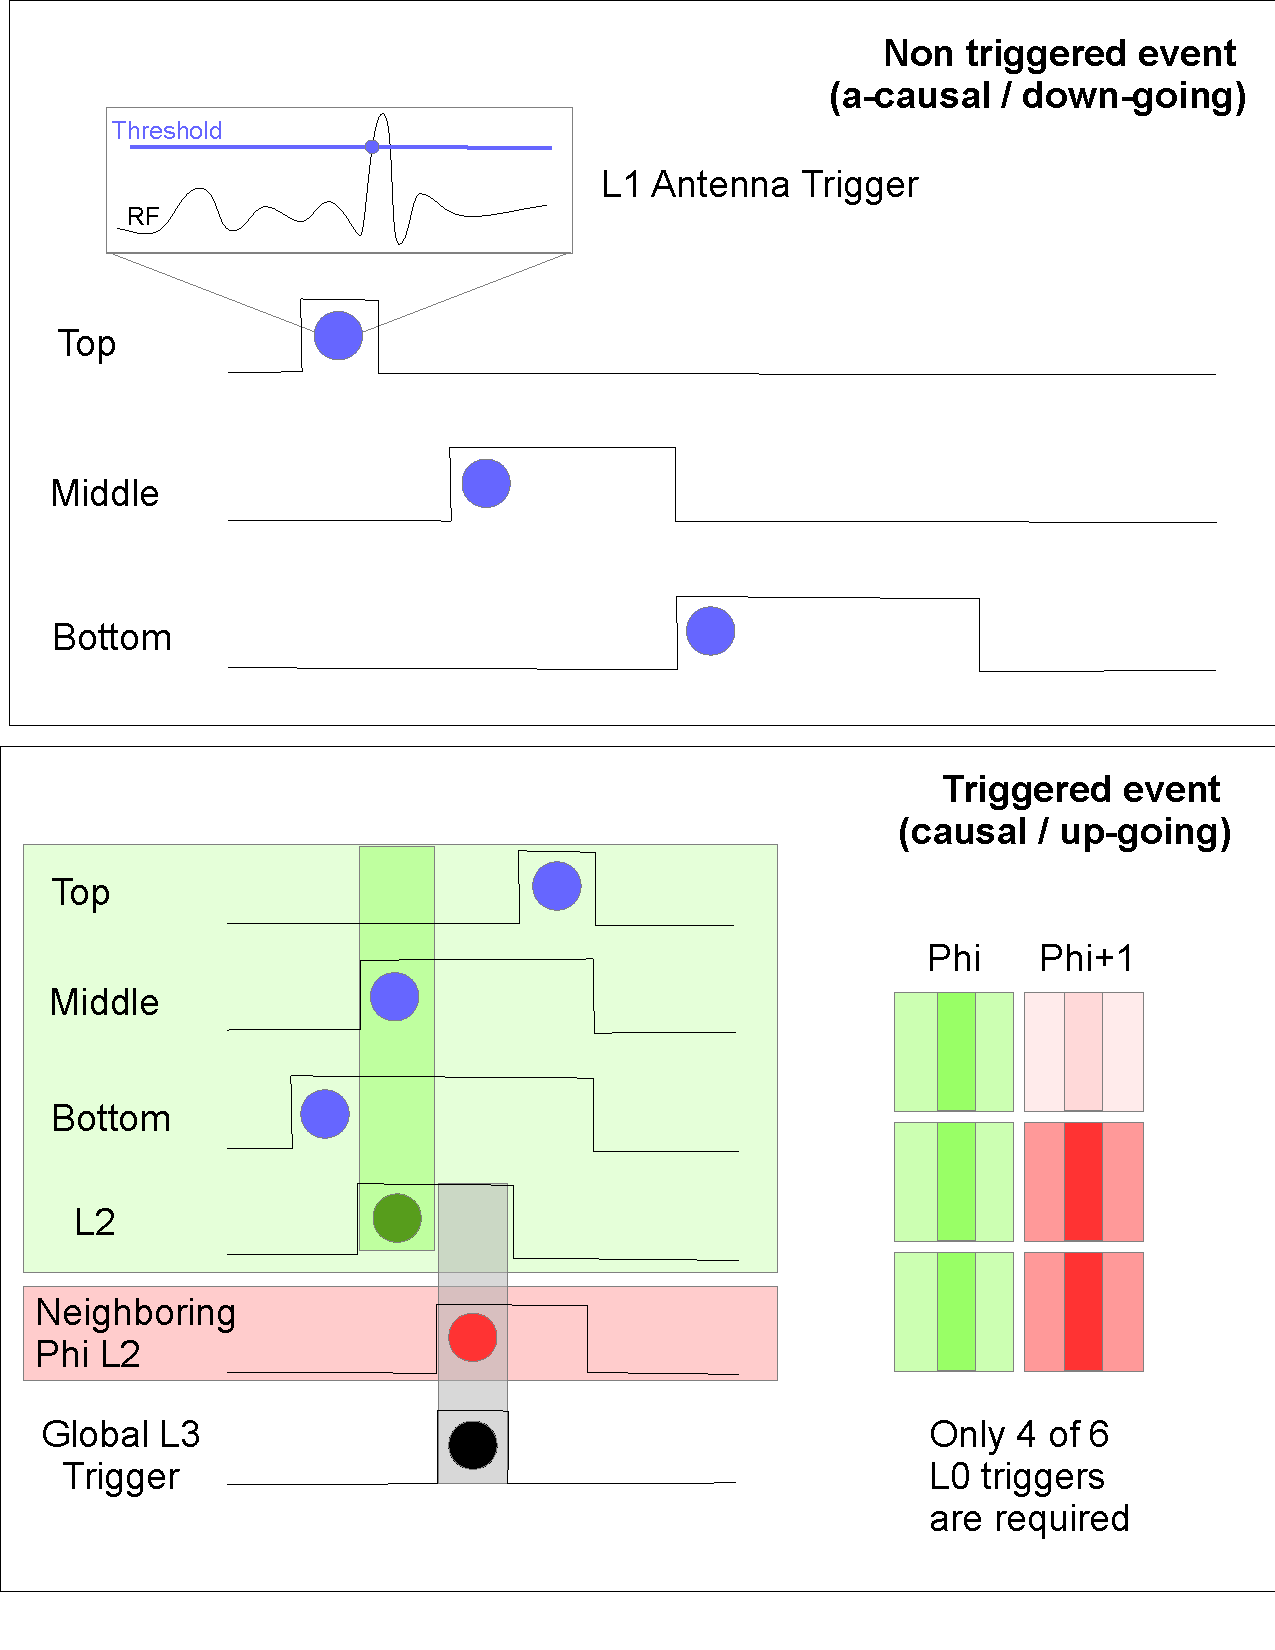
\includegraphics[height=0.8\textheight]{figures/triggerHeirarchy}
	\caption{A depiction of the trigger hierarchy for a non-triggered (top) and triggered (bottom) series of L0 triggers.  The blue dots denote an L0 trigger, and the green box represents the time of a L1  trigger.  Note the 4ns top ring window, the 12ns middle ring window, and the 16ns bottom ring window.  Two neighboring phi sectors with L1 triggers within a 8ns window cause a global trigger (black).  Note also that, though not the case of depicted event, only two of the three rings are required to be in coincidence leading to a 4 out of 6 channel L0 trigger in two neighboring phi sectors}
	\label{fig:trigPattern}
\end{figure}
		
	\subsection{L1 Trigger Window Delay Limitations}
		As the physical offsets between the rings of antennas exceeds one clock period for most of the angles of interest, it is possible to require a timing separation between the arrival of pulses between the separate antennas.  This modification, made between the ANITA2 and ANITA3 flights, decreases the incidental rate of the trigger, increasing the quality, while maintaining the signal rate and efficiency.  This is accomplished by generating a 16ns (four FPGA clock cycles) high logic pulse after a bottom ring antenna L0 trigger, a 12ns (three FPGA clock cycles) high logic pulse after a middle ring L0, and a 4ns window after a top ring L0.  The requirement for a L1 trigger is that two of these windowing pulses overlaps (see Figure \ref{fig:trigPattern}).  This has the unfortunate side effect of allowing the bottom ring of antennas to unfairly bais the system, as a noise L0 trigger generates a pulse with four times the time weight as one from the top ring, and is thus more likely to trigger the system.
		
	\subsection{L2 Multiple Phi Sector Trigger}
		The final L2 trigger is generated when two or more neighboring phi sectors report an L1 trigger within an 8 nanosecond window.  Once the L2 trigger is reported, the TURF board sends a HOLD command to all SURFS, which propagates to a single LAB and initializes a readout.

	\subsection{Phi Sector Masking}
		In the ANITA1 flight, it was discovered that noise sources on the continent and in the sky had the capability to dominate the trigger rate and effectively blind the entire payload despite a large fraction of the payload observing a thermal environment. To alleviate this issue, a system where an antenna or collection (phi sector) of antennas experiences a comparative increase in trigger rate in comparison to the rest of the payload, it will be excluded from forming the global system trigger.  This allows the instrument to continue observing quiet areas of the continent and increasing the total livetime of the system.  There are additional nuances to this subsystem, including the possibility of very high power noise (or signal) events continuing to leak into the back and side lobes of the antennas from non-masked phi sectors, that need to be taken into account when making a measurement of the total instrumented area for a flight.  During the ANITA3 flight, several unexpected in-band satellite CW signals caused the phi masking to be heavily utilized, which is discussed further in the Cosmic Ray Search chapter.
		
%	\subsection{Differences between previous ANITA flight trigger systems}
%		In addition to changing the number of antennas, each ANITA flight has made modifications to the trigger subsystem in an attempt to increase the efficiency and purity of measured events.
		
%		The ANITA1 instrument 
		
%		The ANITA2 instrument separated each signal channel into 3 frequency sub-bands and one full banded trigger within the SHORT boards, before the tunnel diodes.  The reasoning for this was that neutrino signals are full band; a signal with power dominating a single band would be enough to disqualify an event from being a true signal event.  The requirement for a global trigger was several (how many?) bands, in addition to the full band.  It was decided after the flight that this did not did not decrease the quantity of triggers by a significant amount, and the banding scheme was removed in favor of accommodating additional channels (ANITA2 did not trigger on Hpol and had 8 less antennas than ANITA3, so 56 additional trigger channels were required).  This had the unwanted effect of allowing CW signals from northern satellites to overwhelm the detector during the ANITA3 flight.
		
	\subsection{Unbiased triggers}
		Any waveform readout caused by a global trigger has the systematic bias that it passed the trigger selection parameters.  To measure the thermal noise environment during the flight, two triggers that were uncorrelated to the trigger circuit were employed.  These were a software trigger (also know as the soft-trig) that was issued by the CPU at a frequency of 1Hz, as well as a GPS synced 1Hz trigger controlled by the Pulse-Per-Second (PPS) output of the G12 GPS unit.
		
		All events captured by the payload were marked with a trigType integer that described the source of their trigger decision.  The GPS and soft-trig signals can be easily selected in this way by excluding RF triggers.
		
		
\section{RF Power Monitor}
	An additional digitization of the RF signal is done by a broad band radio frequency power detector circuit.  The fast waveform data only provides 200ns of non-triggered unbiased noise data per second (a 1Hz software trigger and a 1Hz gps trigger), so a monitor that digitized a larger fractional percentage of time was desired.  This was accomplished on the SURF board using a commercial RF power monitor IC that converted the RMS voltage of the input signal into a log-magnitude proportional DC output that was digitized by an ADC and read out with the slow read out housekeeping data.  This system, and the additional physics it provides is discussed at length in appendix A.

	
\section{GPS tracking and orientation sensors}
	Since the payload is attached to a free rotation balloon, the orientation and location of the payload was completely uncontrolled and thus needed to be constantly monitored.  This was primarily accomplished with two co-located ADU5 GPS heading receivers in conjunction with a single G12 GPS system.  These 9 total GPS antennas, read out once a second, provide a constant update for the location and orientation of the payload with a resolution of a fraction of a degree.
	
	\subsection{Magnetometer}
		In addition to the heading information provided by the GPS systems, a magnetometer was attached to the payload and used to measure the vector components of the magnetic field throughout the flight.  This system, coupled with a model for the geomagnetic field, could be used as a functional compass, assuming an accurate position, that would corroborate the pointing information returned by the GPS systems.
		
	\subsection{Sun Sensors}
		Many space borne experiments that require very high pointing and location precision, however are above the altitude where GPS has significant accuracy (is this a thing?), use star sensors to orient themselves.  ANITA's flight path over Antarctica during the austral summer, specifically the continual daylight, is able to use just one star to obtain accurate heading information.  With an accurate time and knowledge of the earth's rotation around the sun, one can use a simple pinhole camera and the four mounted angular sun sensors to determine the heading information for regions of time when the GPS is unavailable or unreliable.
		
\section{CPU, CPCI, and Data Readout}
	The custom LABRADOR digitizer ASICS and various control and command FPGAs are located on custom designed printed circuit boards (PCBs) connected to a central processing unit (CPU) over a compact peripheral component interconnect (cPCI) bus interface.  
	
\section{Data Storage and Telemetry}
	The most important piece of any experiment is the storage of the measurements for later analysis.  The quantity of data taken during flight saturates the hard-linked digital hardware used to read it out and store it, and thus it is not feasible to downlink the entirely of the stored information during flight.  This necessitates the recovery of the payload, or at least the storage vaults, immediately preceding the flight.

	\subsection{Redundant data storage}
		The storage requirements for the flight were met by three separate and unique digital storage formats.  This redundancy ensured that even in the event of a single failure the data from the flight would be preserved.  The first storage method was two identical Helium filled conventional spinning hard disk drives written to by the flight CPU over SATA.  The second method was a separately housed array of six solid state drives written to by a dedicated single board computer which received the flight data over an Ethernet link.  The third storage method, which ended being flown in an inactive state, was the RIFFRAFF handheld flash drive array; a complex system of microcontroller steered multiplexed commercial USB flash drives visible to the flight CPU.  During flight, a failure of the Ethernet link lead to the loss of the SSD array subsystem, leaving only the He Drive storage format intact.  Both drives survived the flight however, and two identical copies of data were recovered.
		In ANITA-III, the NTU device was a standalone CPU that connects with the flight CPU over ethernet and connected to six 1TB SSDs.  When one filled up, it would flip to the next.  It stopped communicating like a third of the way into the flight (probably because the ethernet power cable wiggled loose and all ethernet connectivity ceased), and was not ever required due to the success of the He drive system.
		
	
	\subsection{Telemetry}
		Downlink of data taken during flight and uplink of commands to change flight configuration are transmitted to and from ground receivers over several systems.  In order of decreasing data trasmission speed, they are the Line Of Sight (LOS) transmitter, an Iridium Pilot\textregistered Openport UDP link, a NASA Tracking and Data Relay Satellite System (TDRSS), and an Iridium\textregistered low rate downlink.  These systems allow in-flight diagnostics of the ANITA3 instrument, as well as an ability to make pre-defined alterations to instrument control configurations depending on need.  Shortly after flight, the Iridium Pilot\textregistered Openport link failed for unknown reasons.  However, the remaining systems were successful in allowing flight operators to debug and fix several issues that cropped up during the flight.
		
	\subsection{GPU prioritization}
		The data limitations of the various telemetry downlink systems allow only a fraction of the total data rate to be transmitted.  This limitation motivates a prioritization system in order to only send down events that pass a limited set of post-digitization analysis cuts.  This would allow a limited set of analyzable signals in the event of a catastrophic system failure or non-recovery of the payload.  The two major figures of merit for discriminating between incidental thermal noise events and impulsive signal-like events is the normalized peak height of an interferometric pointing map, and the peak of the Hilbert envelope of the coherently summed waveform for the respective map peak incidence angle.  These time-consuming, computationally intensive, physical baseline dependent, multiple channel correlation processes are nominally done offline in the analysis phase of the experiment, and is likewise further discussed in the analysis chapter of this thesis.  However, to accomplish the task in real time as events are streaming from the instrument, a Graphical Processing Unit (GPU) linked with the flight CPU was utilized to parallelize the computations and reduce any specific event readout's required processing time to that of the minimum instrument readout time.  These values were then used to determine a priority for each event and placed in an appropriate telemetry queue.  The main work on this system was done by Ben Strutt of University College London, and details on its operation and results can be found in his thesis at \cite{BenSThesis}.  Since the instrument was recovered, these computations are re-done for this thesis, and the priority value was not used.
		
	\subsection{Balloon}
		The ANITA instrument is suspended by a NASA zero pressure long duration high altitude balloon.  This balloon is cool.
			
			
			
			
%%%%%%%%%%%% 3 %%%%%%%%%%%%%%%%%%%%%%%%%%%%%%%%%%%%%%%%%%%%%%%%%%%%%%%%%%%%%%%%%%%%%%%%%%%%%%%%%%%%%%%%%%%%%%%%%%%%%%%%%%%%%%
\chapter{Instrument Calibration}
%%%%%%%%%%%%%%%%%%%%%%%%%%%%%%%%%%%%%%%%%%%%%%%%%%%%%%%%%%%%%%%%%%%%%%%%%%%%%%%%%%%%%%%%%%%%%%%%%%%%%%%%%%%%%%%%%%%%%%%%%%%%

	The measurements recorded by the ANITA3 digitizing electronics need to be calibrated and the instrument geometry must be precisely measured in order for observed events to be directly relatable to the electromagnetic field present at the instrument.  There are several major considerations that have to be taken into account in order to properly calibrate the instrument.  The LABRADOR ADC counts need to be scaled to voltage, the sampling time base has to be corrected for uneven sampling rate, the gain and phase of the impulse response to the system has to be measured, and the actual physical locations of the antennas has to be measured and corrected from the engineering model.  The end goal of any calibration is to relate the measured and recorded quantities, by parameterizing the observation instrument and using known values to calculate those parameters, to the actual physical effect that is being observed.  The following chapter details the steps taken and results of calibrating these aspects of the ANITA3 instrument.
	

	
\section{LABRADOR voltage calibration}
		The LAB3 ASCIC uses a ring buffer storage capacitor array (SCA) to store many sequential snapshots of the charge on a capacitor from a time varying electrical potential arriving at the chip.  This captured analog charge is then digitized (an analog to digital conversion, or ADC) by comparing it to a constant current source ramp signal that stops a Wilkinson clock at the time of comparator activation (see Figure \ref{fig:Lab_Digitization}.  The digital values read out by the acquisition software are then physically measuring a time between when the ramp signal begins and when it's voltage passes the voltage of the stored charged in that particular SCA bin.  This ADC count must be converted into a voltage that can be propagated back through the signal chain and inform us on the induced potential on the antenna.

\begin{figure}
	\includegraphics[width=\textwidth]{figures/LAB_Digitization}
	\caption{Simplified diagram of the digitization chain for the LABRADOR3 digitizer}
	\label{fig:Lab_Digitization}
\end{figure}	
		


	\subsection{Pedestal Subtraction}
		The signal propagated through the ANITA3 system is AC-coupled by design, and as such must have a DC offset reintroduced to it before being being digitized by the LABRADOR.  The ramp voltage and comparator internal to the chip operate only at positive voltages (0 to 2.5V) , and so to get a measurement of both positive and negative voltage fluctuations the signal must nominally be set at mid-range of the ramp signal, or about 1.25V.  This is accomplished through a fixed voltage regulator external to the LABRADOR on the SURF board.  This "pedestal" voltage, visible in the data as a constant ADC count offset, must be later subtracted to correctly zero mean the signal.  A "pedestal run," in which large numbers of samples were measured and averaged to determine a mean value per capacitor bin, was done at the beginning of the flight and stored on a storage drive of the instrument.  These pedestals were then subtracted immediately after captured by the acquisition software (Acqd) before being stored, and are included in the raw data.  The pedestals used in ANITA3 are visible in Figure \ref{fig:pedestals}
		
\begin{figure}
	\centering
	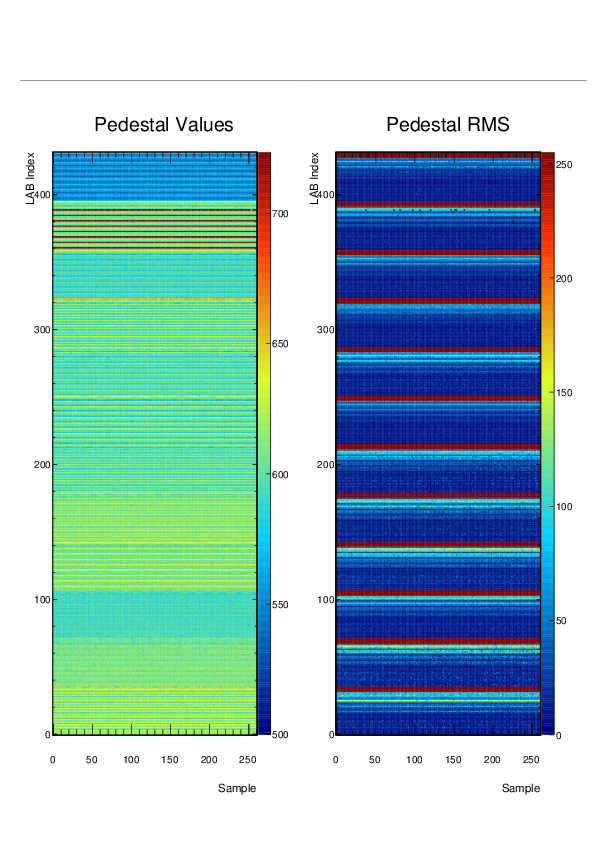
\includegraphics[height=0.8\textheight]{figures/Pedestals_big2}
	\caption{Mean pedestal values used for subtraction(left) and RMS of bin in pedestal run (right) for all LABRADOR chips for the ANITA3 flight.  The Y axis is an index describing the LABRADOR in question (SURF*36 + Chan*4 + Lab,).  The X axis is the capacitor bin number within that surf.  The Z color axis is the value of the Pedestal or RMS in ADC counts.  From this plot one can visibly see the small variance of pedestals within a single LAB, but moderate variation between SURFs.  Also visible is the clock channel and its associated large pedestal RMS, as the clock remains on during pedestal runs.}
	\label{fig:pedestals}
\end{figure}	
				
				
	\subsection{Least Significant Bit Masking}
		As a note, though the LABRADOR reads out a 12 bit digitized ADC value, the least significant two bits are known to be systematically biased and are thus masked.  The final ADC value stored by the acquisition software is an 11 bit signed integer, with the least significant bit determined by the pedestal correction.  This means that bins have either even or odd values, but not both.  This effect can be seen in Figure \ref{fig:evenOddPeds}.  Functionally it allows the pedestal to have half bit resolution while not requiring float arithmetic for further CPU tasks.
		
		
	\begin{figure}
		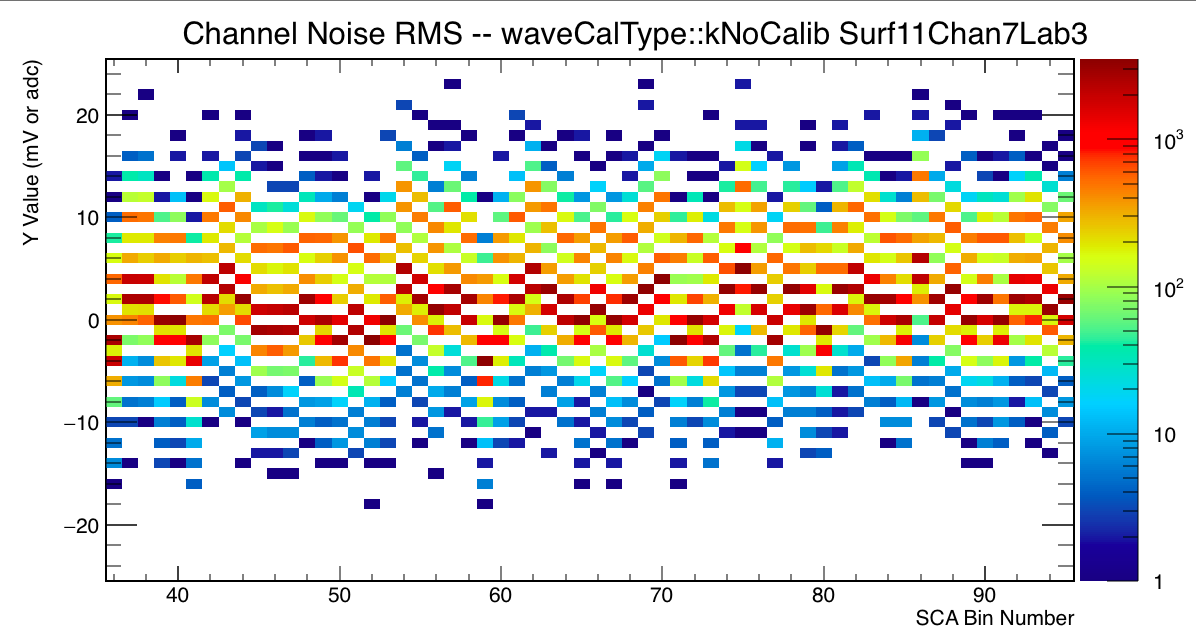
\includegraphics[width=\textwidth]{figures/pedsEvenOdd}
		\caption{A histogram of ADC count occupancy as a function of capacitor bin stored by the acquisition software.  The least significant bit from the LABRADOR is masked to zero, however the constant pedestal subtraction has a LSB addition that causes an offset.}
		\label{fig:evenOddPeds}
	\end{figure}
		
	
	
	\subsubsection{Simple Voltage to ADC Count Calibration}
	To initially measure the voltage to ADC counts of the LABRADOR chips an identical RF pulse was inserted into two AMPA channels at the front of the signal chain, then measured both after the full signal chain immediately before entering the SURF RF input with a calibrated Tektronix oscilloscope, and using the ANITA readout software (See Figure \ref{fig:calSetup}, note this figure is used in multiple calibration analyses). This signal was then compared against the pulse read out by the acquisition software.  While keeping the reference channel constant, the test signal was then moved throughout the remaining 95 channels.  The peak to peak signal height of each test channel was then compared against the reference channel's oscilloscope readout.
		
			
	\begin{figure}
		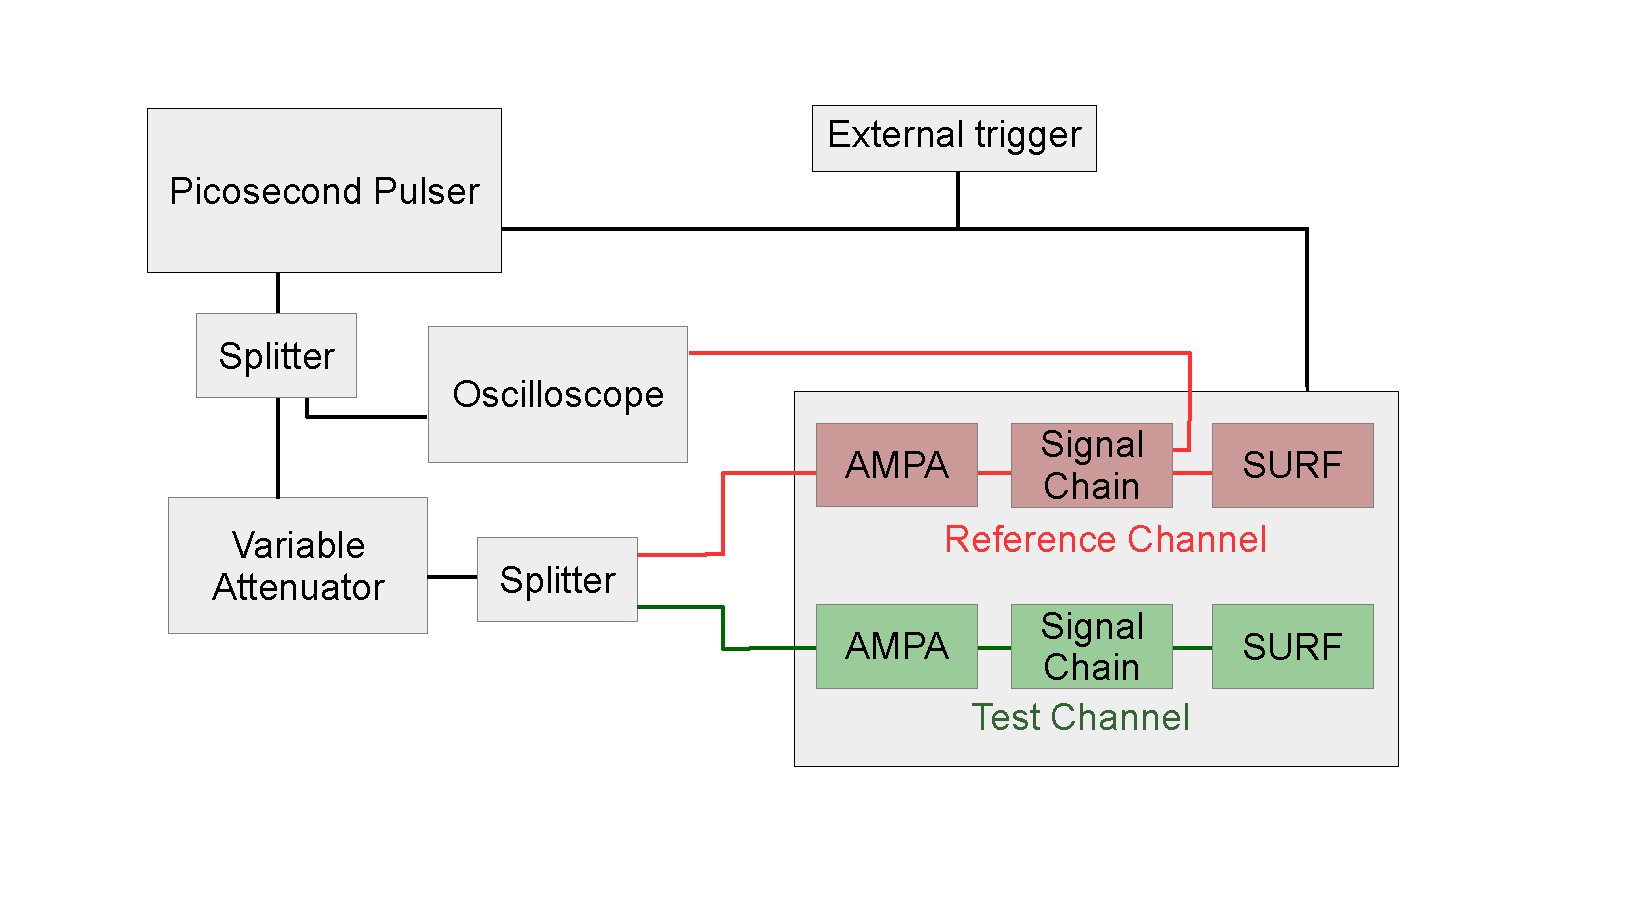
\includegraphics[width=\textwidth]{figures/antarctica14_calSetup}
		\caption{A schematic of the pulse insertion calibration setup used immediately before flight with the full signal chain in Antarctica in 2014}
		\label{fig:calSetup}
	\end{figure}
		
	One drawback of this method is that only the reference channel is coupled out from after the signal chain for comparison with the SURF output pulse.  This pulse is dispersed by the amplification and filtering of the signal chain, and thus comparing it to the input pulse requires the full complex impulse response, which considers both gain and phase as a function of frequency of the system, an analysis that is described later in this chapter.  For a simple first-order voltage calibration, one assuming voltage to be a linear function of ADC counts with no frequency dependance and an identical complex impulse response between signal chains, the peak to peak amplitude of each test channel compared to the reference channel is sufficient.  However, since the magnitudes of the gains of the signal chains is not equal, this calibration serves best as a normalization between the full signal chains of all the channels.  In other words, after applying the simple volts to ADC counts calibration, all channels are expected to have equal peak to peak voltages for an identical input signal regardless of signal chain gain or noise figure.
		
		
		
	\subsection{Chip to Chip Variation}
		Each chip suffers from manufacturing non-idealities introduced by the nano-lithography process.  Due to this, each chip must be calibrated independently.  The time base generator, the write pointer strobe propagation and RCO phase dependance, as well as the ADC to absolute voltage values must all be independently measured for each chip.  The resulting ADC counts to mV conversion can be seen in Figure \ref{fig:adcTomV}.

			
	\begin{figure}
		\centering
		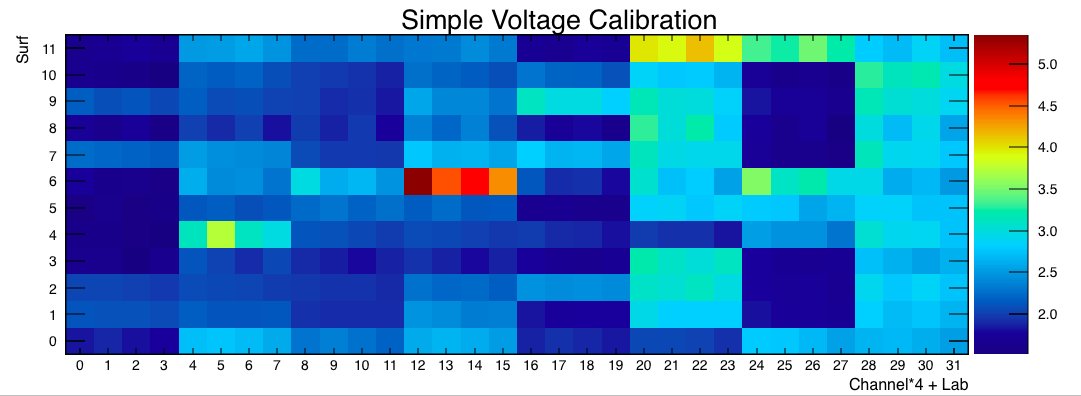
\includegraphics[width=\textwidth]{figures/ADCtoVolts.png}
		\caption{Simple voltage calibration values for all 96 channels of the ANITA3 instrument (taken from simpleVoltageCalibrationHarm.txt).  The units of the Z-axis color bar are in mV/ADC counts.  Note that each channel is digitized by four separate LAB chips.  However, the largest effect on the voltage calibration is from variations in the signal chain}
		\label{fig:adcTomV}
	\end{figure}
		



\section{LABRADOR timing calibration}
		The LAB3 storage capacitors' time base are controlled by a series of current starved transistors propagating a pulse down the array.  This allows each cell to be periodically and sequentially connected to the input signal, then disconnected  which can then be later digitized.  This timing generator circuit is effected by non-idealities of the ASIC manufacturing process as well and thus does not create equally spaced time separations between capacitors in the sampling array.  The timing separation, or delta-times (dTs for short), of each sample is shared between all eight channels of each LAB chip as it is generated by the same timing generator, however it can have significant variance between the different chips within a single SURF as well as between the SURFs.  There are 96 total lab chips actively recording data in the ANITA3 instrument, and each must be calibrated for this dT variance.

\noindent		
\begin{figure}
	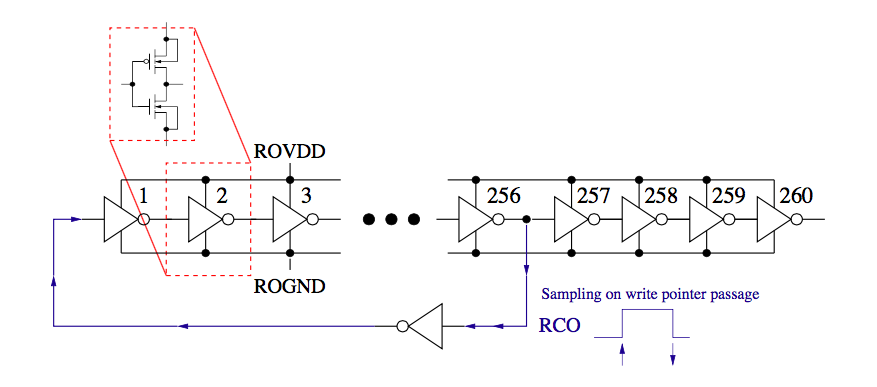
\includegraphics[width=\textwidth]{figures/LAB3BTimingGenerator}
	\caption{Diagram of LAB3B timing generator circuit\cite{LABASICPAPER} }
	\label{fig:timingGenerator}
\end{figure}

	\subsection{Time Domain Bin Width Matrix}
		The time base generator is comprised of a series of 260 current starved transistors that propagate a write strobe across the entire SCA.  Since each transistor has differing characteristics due to the non-idealities of ASIC manufacturing, this strobe does not evenly pass from time bin to bin.  This necessitates a "dT" calibration constant for each of the 260 samples, as well as for each phase of the write strobe (up-going or down-going), leaving us with 520 total calibration constants per LAB.  There are several methods that can be utilized to determine the timing separation between any two capacitor bins, two of which were used to check the calibration of the ANITA3 instrument.
		
	\subsubsection{Bin Occupancy Fraction Method}
		
		The first calibration technique I will refer to as the Bin Occupancy Fraction method.  This method involves injecting a constant periodic signal, either a digital clock or a constant frequency sine wave, into each of the LAB chips.  By recording a large number of events, we can measure the resulting number of zero crossings that occur between each capacitor bin pair.  By comparing this occupancy vs the expected occupancy for a uniformly sampled time window in which each bin observes the same number of zero crossings, it is possible to determine the fractional width of each bin.  A drawback of this method is that it requires very large statistics to reduce the uncertainty on the resulting dT.  
		
		This calibration was done for ANITA3 with two timing sources, an injected 432.1MHz sine wave and the 33.3MHz square wave sync clock injected into the system for the entire flight.  The sine wave calibration, preformed by Ben Strutt and detailed in his thesis (\cite{benSThesis}), is the nominal calibration that is used for the remainder of this thesis.  The array can be seen in Figures \ref{fig:dTNominal2D} and \ref{fig:dTNominal2D}.  All other bin width matrix timing calibrations detailed below were done as a check on those values.
		
	\begin{figure}
		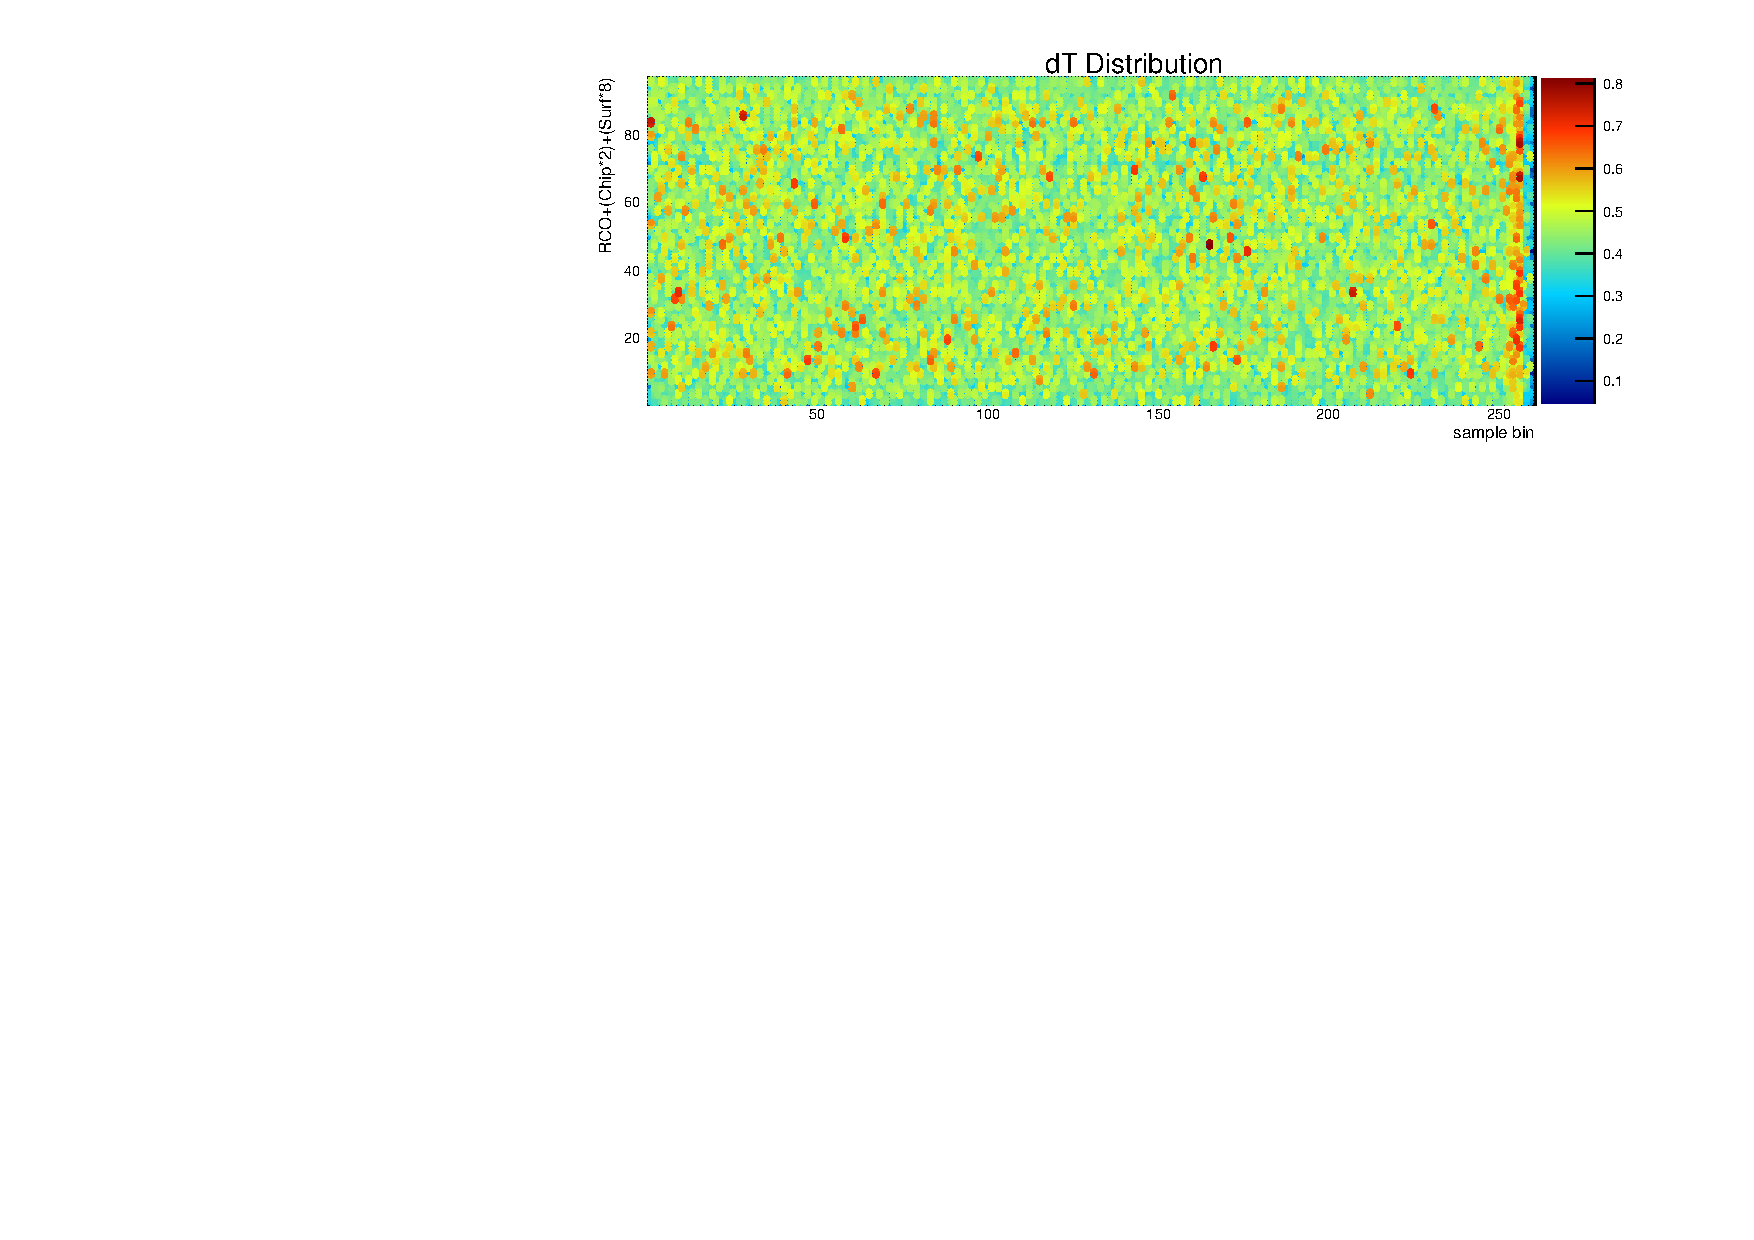
\includegraphics[width=\textwidth]{figures/dTNominal2D}
		\caption{Nominal LAB3 Time Domain Bin Width "dT" values generated using a 432.1MHz injected sine wave calibration signal and the bin occupancy fraction method.  Values were determined by Ben Strutt\cite{benSThesis}.}
		\label{fig:dTNominal2D}
	\end{figure}
	
	
	\begin{figure}
		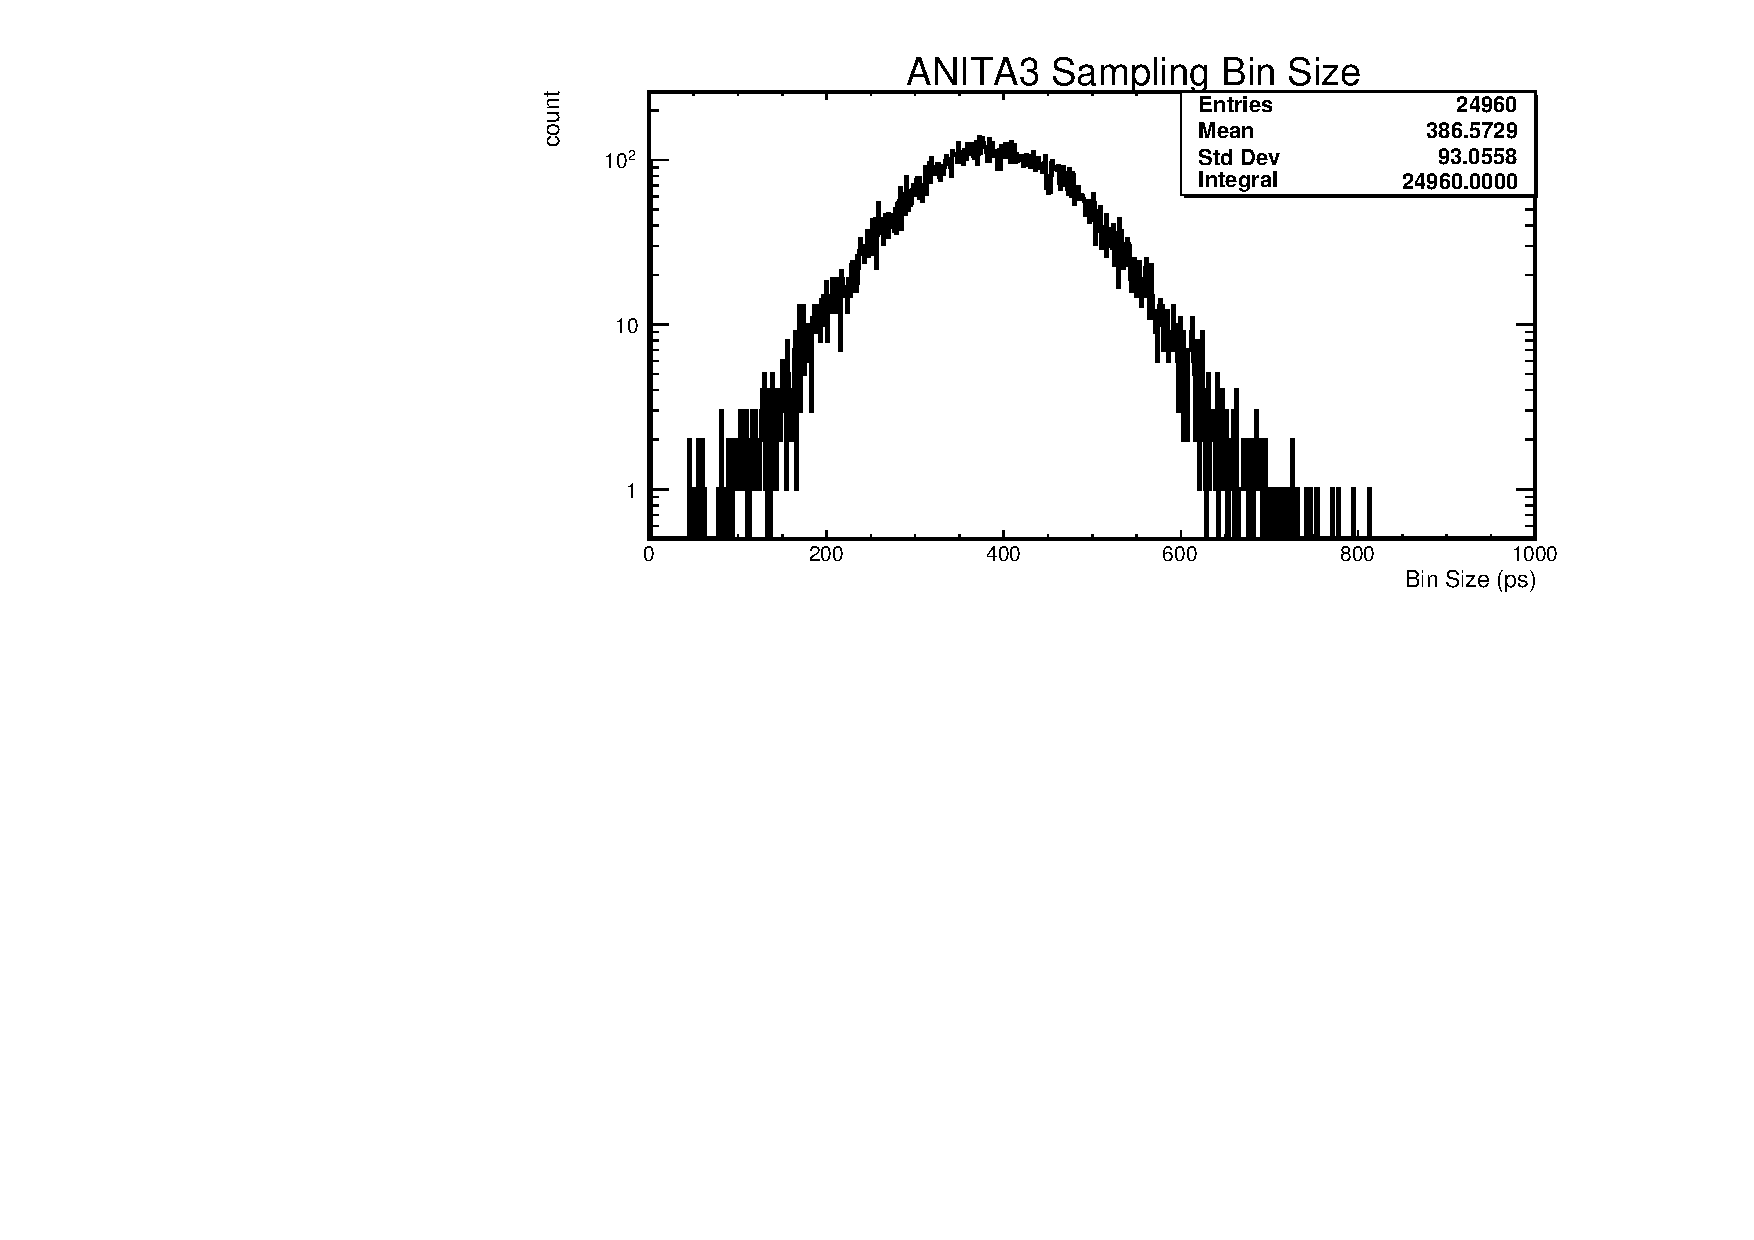
\includegraphics[width=\textwidth]{figures/dTNominal}
		\caption{Nominal LAB3 Time Domain Bin Width "dT" values generated using a 432.1MHz injected sine wave calibration signal and the bin occupancy fraction method.  Values were determined by Ben Strutt\cite{benSThesis}.}
		\label{fig:dTNominal}
	\end{figure}
		
		The second possible calibration source, the 33.3MHz sync clock, is also useful for this calibration method.  It has the additional benefit of being constantly present throughout the entire flight.
		
		
	\begin{figure}
		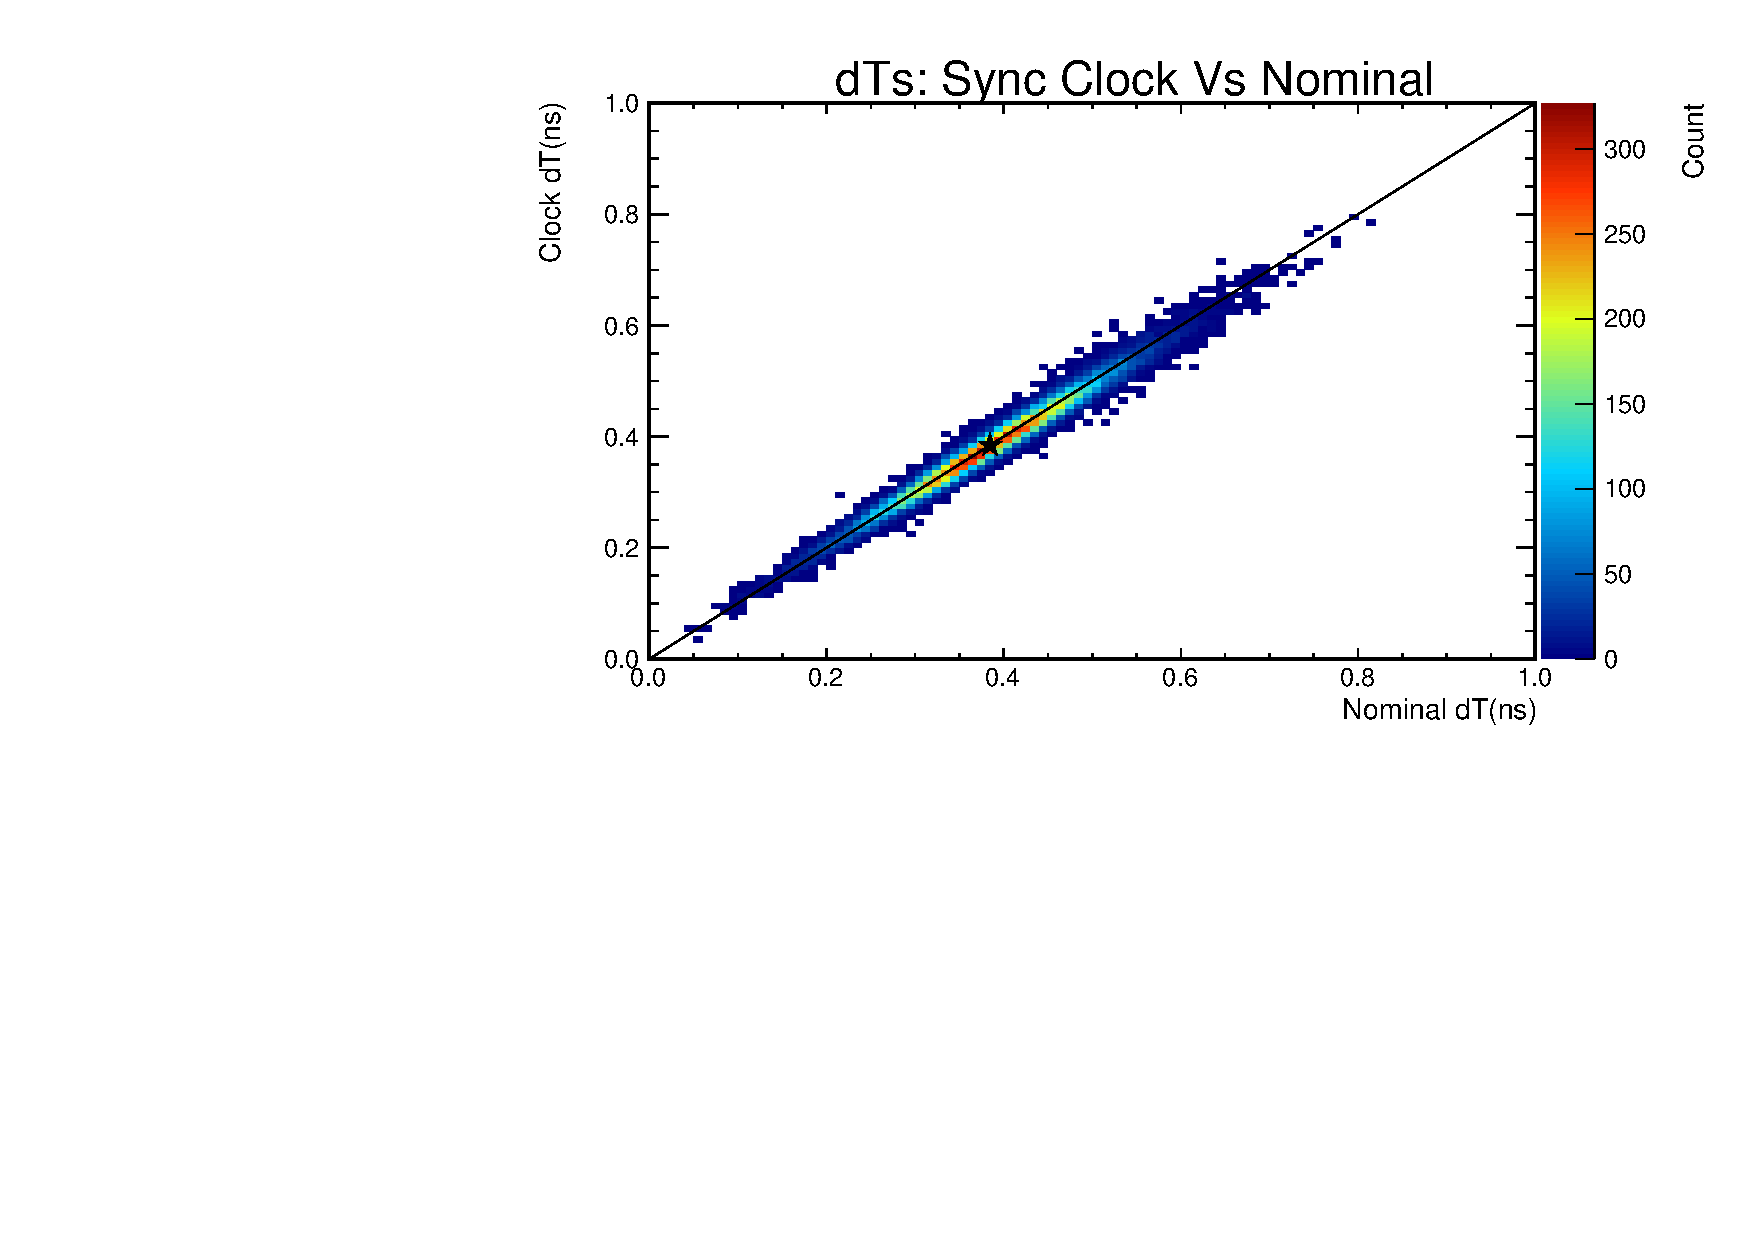
\includegraphics[width=\textwidth]{figures/nominalDtVsSyncClockDt}
		\caption{Comparison of the }
		\label{fig:dTNominal2D}
	\end{figure}



		
		
		

	\subsubsection{Ellipse Method}	
		The second calibration technique is slightly more clever, and involves utilyzing a characteristic of a significant number of phase offset sine waves captures and will be called the Ellipse method.  Plotting the sum and difference of sequential samples of a pure sinusoidal function yields an ellipse whose semi-major and semi-minor axes determine the fractional time of each sample.  
		
		Using this method, whose derivation is detailed in Appendix B, it is possible to determine the width of each bin by comparing the sum and difference of digitized values from neighboring bins that are offset by some time $\delta t$ both observing the same sine wave.  It is useful to consider the edge cases of such a system, for example two bins that have a negligible dT separation.  In this case the measured voltage difference between them will always be small if not zero, while the addition axis has a can a large range of values, the maximum being the crests of a sine wave. This will yield an ellipse with a very large eccentricity.  Inversely will have the inverse eccentricity, bins that are separated by exactly one half wavelength of the injected frequency will always have wide range of possible differences, and sums always approaching zero.  Nominal sampling between these extremes will provide an ellipse approaching a circle, as seen in Figure \ref{fig:ellipseMethodExample}.  This method is useful in that it requires far less data than the Bin Occupancy Fraction method.  
		
		Utilyzing this method, I calibrated all capacitor bin dTs and compared the results with the previously measured constants provided in this thesis and other published results\cite{benSThesis}.  The values are presented in Figure \ref{fig:ellipseResults}.
		
	\begin{figure}
		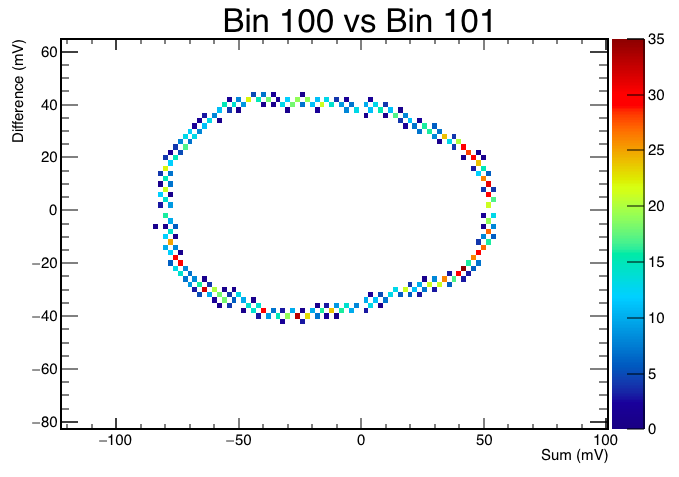
\includegraphics[width=\textwidth]{figures/ellipseMethodExample}
		\caption{}
		\label{fig:ellipseMethodExample}
	\end{figure}

	\begin{figure}
		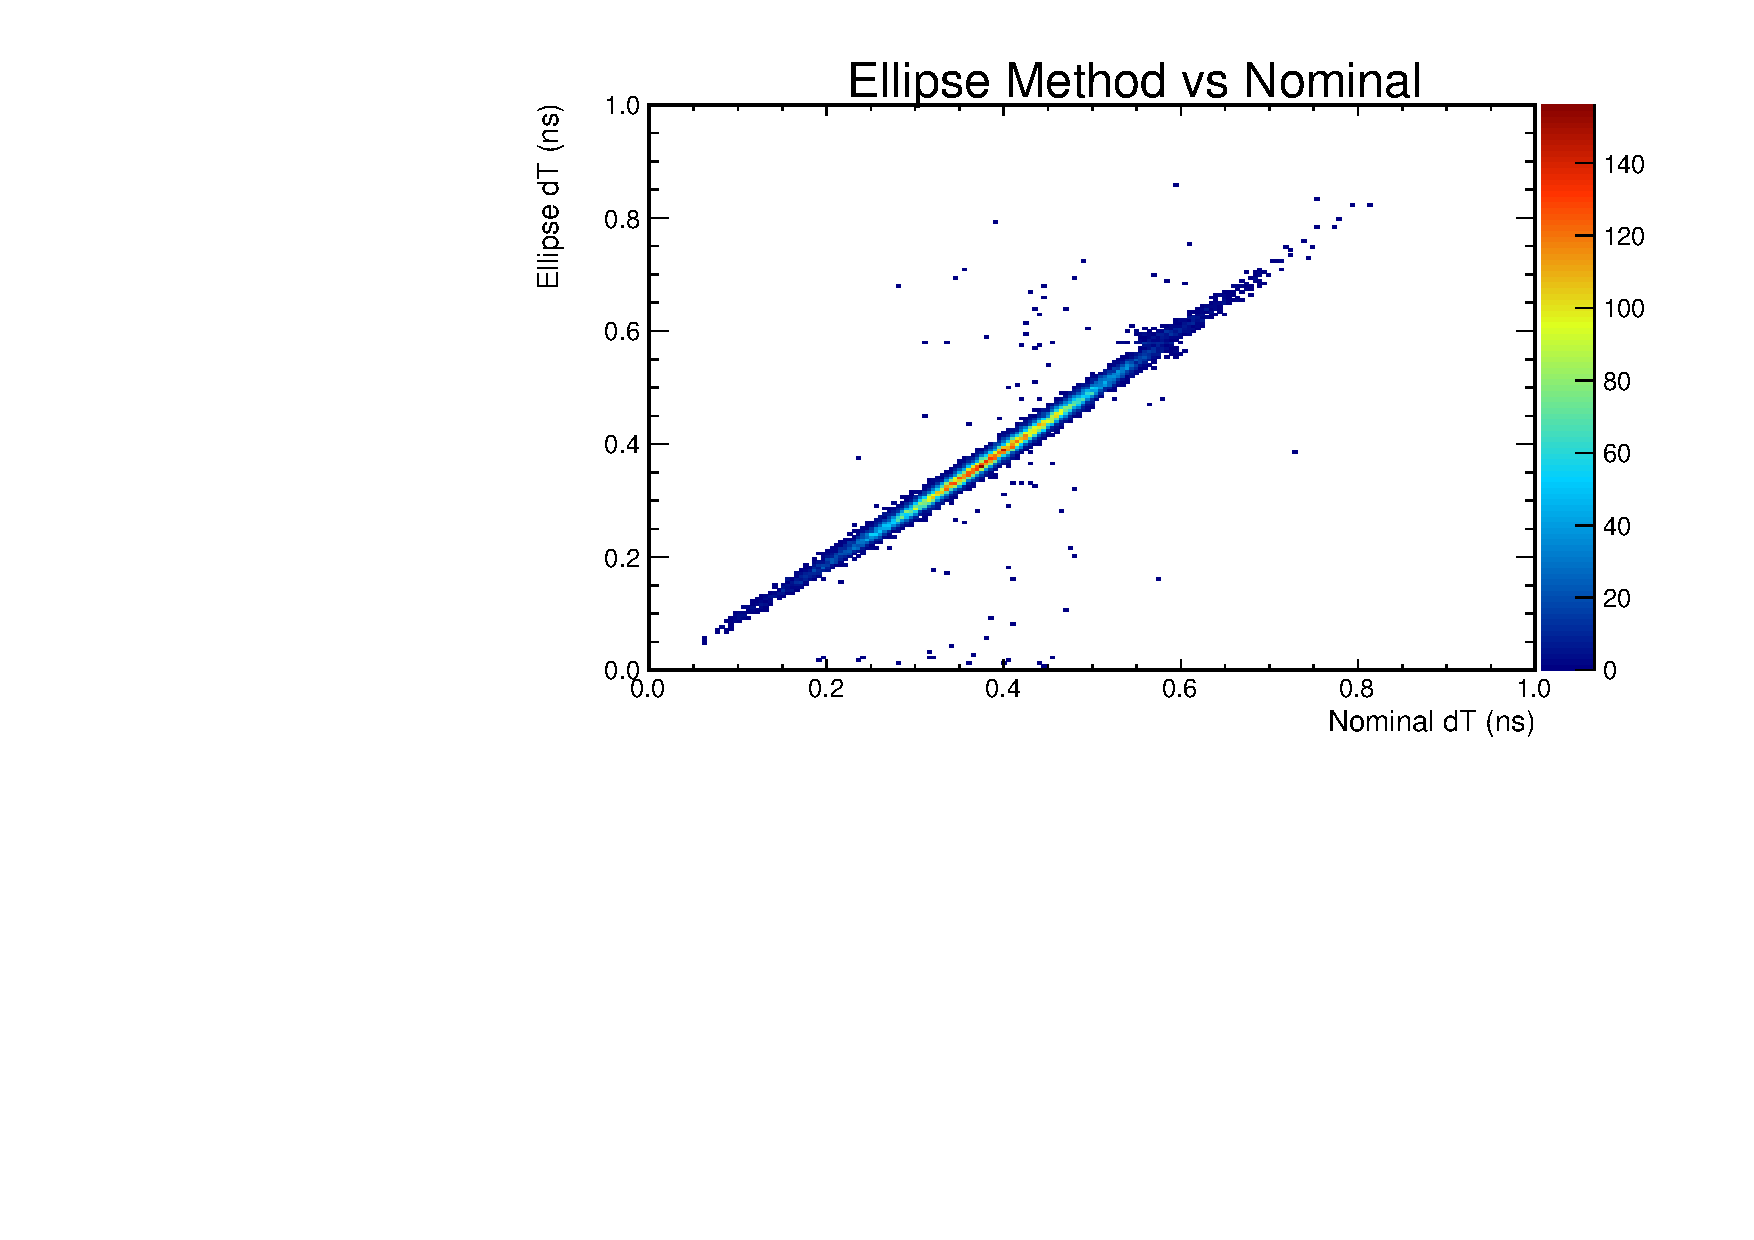
\includegraphics[width=\textwidth]{figures/ellipseComparison}
		\caption{}
		\label{fig:ellipseResults}
	\end{figure}


	\subsection{Sine Wave Fitting Method}
	
	There exists a third method for calibrating each digitizer bin's timing width, which is applying an iterative least-squares fit of the inserted sine wave and determining the relative phase offsets of the voltage of each recorded point versus the same value of the fit.  This was done as an additional method for determining the validity and event to event stability of the dT constants.  This method has the additional benefit of requiring extremely low statistics, with a measurement of the width possible on a single captured waveform.  Of course, the four LAB buffer and dual RCO phases results in each bin only being measured one eighth of the total event read out.  Additionally, the only periodic input function was a sine wave which has a large fractional region where small voltage offsets effect large timing offsets, or regions where the derivative is small.  The bin occupancy fraction method is in a way a simplification of this method, using only times where the derivative is largest.  
	
	


	\subsection{dT Variance and Timing Results}	
		The variance in the timing from bin to bin has a strong effect on the measured bandwidth of the system.  Due to the non-periodic nature of the signal, bins that are sampled too far apart will be unable to digitize frequencies that are higher than the Nyquist frequency of the pair.  Similarly, samples spaced closer together than the nominal sampling frequency will act to alias in high frequency noise and dilute the signal.  The nominal sampling variance between the ANITA1 and ANITA2 flights increased by a factor of 3.5 to 25\%, which reduces the signal power in the high end of the spectrum .  The cause of this change between the ANITA2 and ANITA3 flights is unknown.
		
		
	\subsection{Wraparound Time ($\epsilon$)}
		The propagation time of the write strobe between the end of the SCA and the beginning is longer than a single bin.  As the SCA acts as a ring buffer, and the pulse can occur at any time within the SCA, the write strobe must begin its transition back to the first bin before the end of the SCA, at bin 256.  The remaining four bins are then used to fill in the "wraparound" time, which has been colloquially called $\epsilon$.  These epsilon values also differ with each RCO phase, and so each chip receives two $\epsilon$ correction constants. In addition, four dT periods is often longer than the wraparound time, and as such the 260th sample is often treated as a duplicate and discarded.  
		
	\subsection{RCO Phase and Determination}
		The RCO phase is sent as an output to the FPGA as a buffered copy of the wraparound voltage.  Using this, it is possible to determine the current phase of the chip when a hold was placed.  This has issues at the boundaries of the SCA, as the FPGA may not have latch the current RCO value when returning the digitized values.  A correction for this can be made by measuring the period of the ninth channel sync clock, which will differ between each RCO phase.  Using the firmware reported value in conjunction with the sync clock period allows for correctly determining the RCO phase with high accuracy.

	\subsection{Temperature Dependance}	
		All transistors react differently to temperature, and those present in the time base generator are no exception.  As the payload cools and warms due to rotation, time of day, and latitude, the sampling frequency will increase and decrease.  To alleviate this, a temperature correction must be applied to the final data. This is done via an average of the CP30 number reported by the FPGA over multiple events.
		

		
	\subsection{Inter-SURF Timing for Waveform Alignment}	
		As each LAB3 runs independently of each other and each channel has different signal chain group delay characteristics, each channel must be aligned in time with each other to determine the precise timing of any digitized waveforms.  The delay between channels has both a time invariant and time varying component on an event by event basis.  
		
		The invariant term, caused by the path lengths of the digitization control signals between the TURF and SURF boards in addition to any group delay offsets introduced by the signal chain, can be initially calibrated out using coincident pulses inserted into multiple channels.  To measure and correct for this offset, an impulse was sequentially injected into each channel while a coupled impulse was simultaneously injected into an unchanging reference channel.  By measuring the difference between the observed arrival times of these pulses at each SURF, it is possible to develop a matrix of constant delay offsets between channels.  This calibration setup is described in Figure \ref{fig:calSetup}.  The results of this calibration are shown in Figure \ref{fig:delayOffsets}.
		

	\begin{figure}
		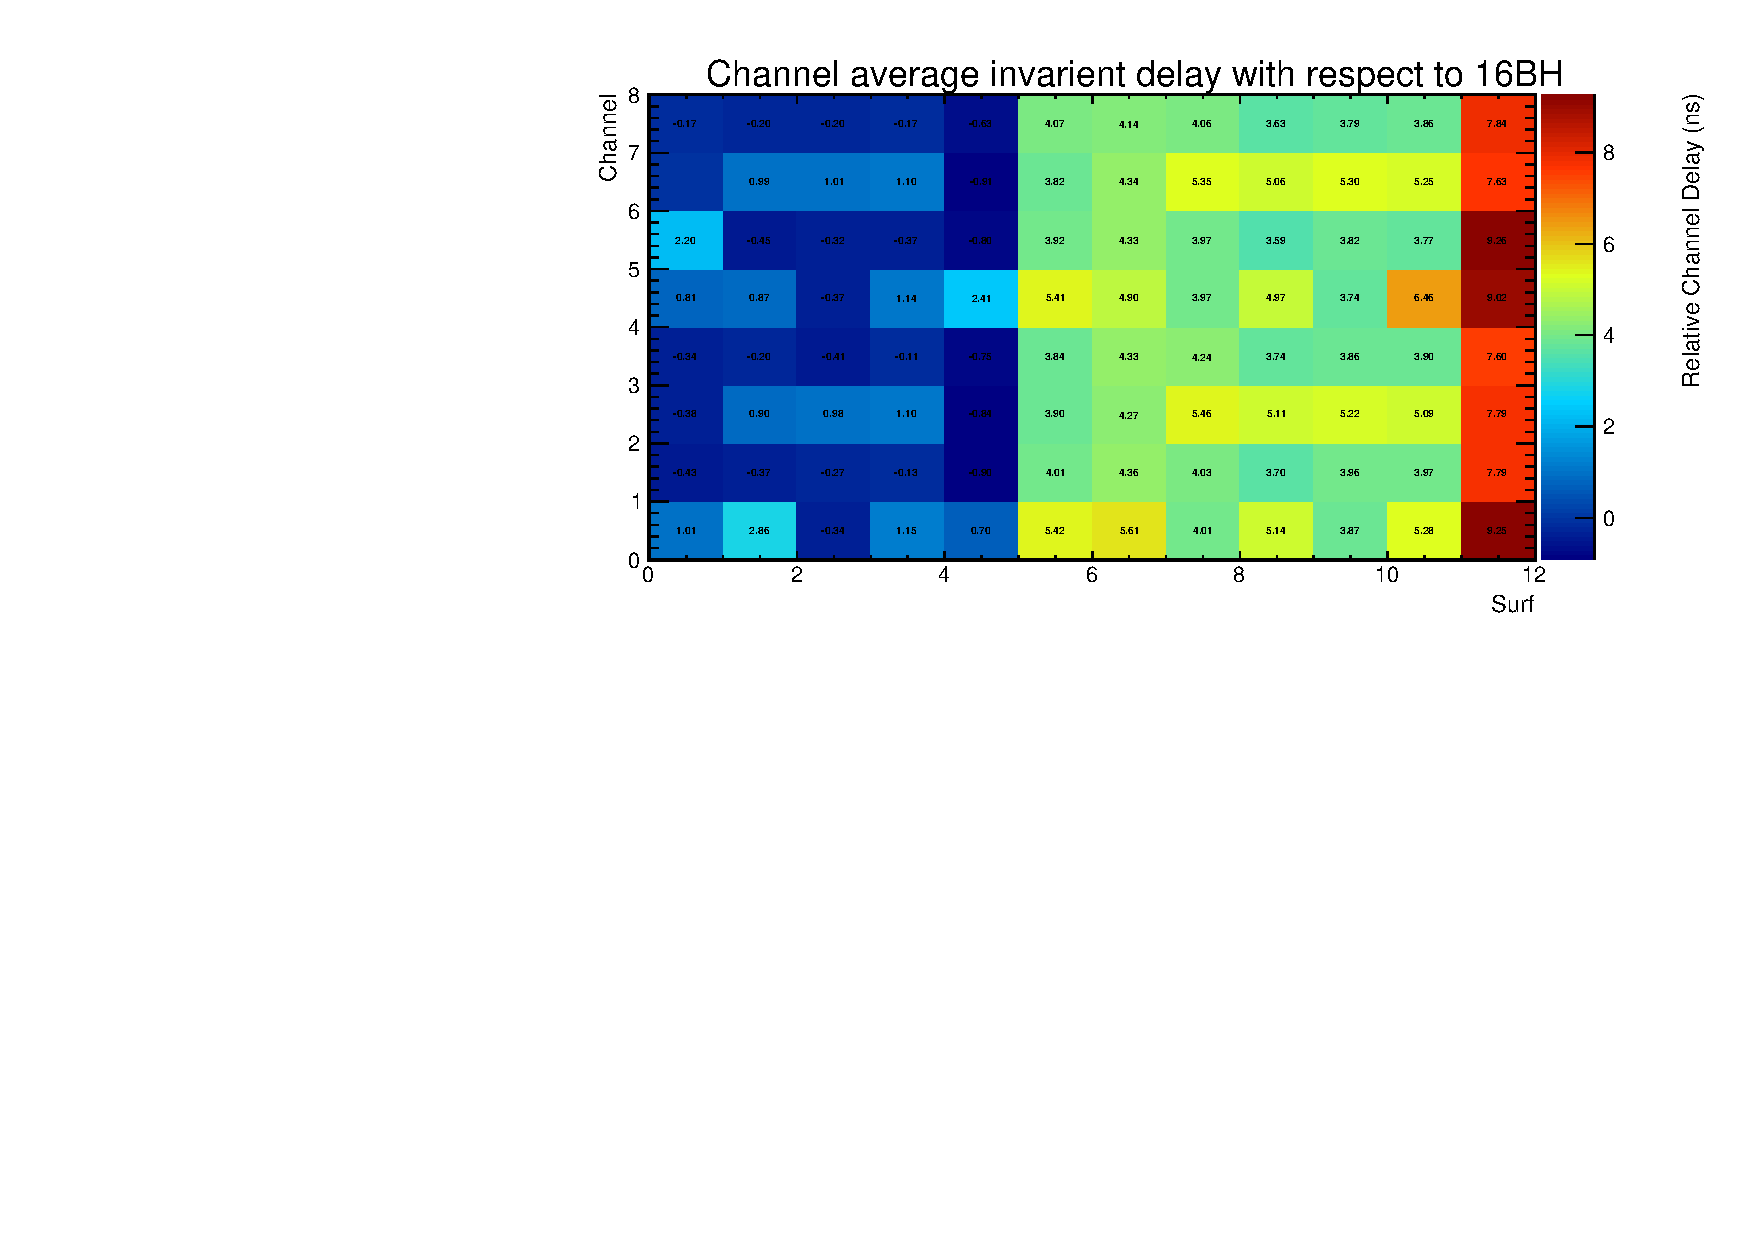
\includegraphics[width=\textwidth]{figures/averagedCableDelay}
		\caption{Channel}
		\label{fig:delayOffsets}
	\end{figure}
		
		
		The event by event time variance introduced by the nature of discrete clocked digital logic and the free-running sampling controls of the LABs, must be done at each event.  This is done with a "sync" clock that is propagated amongst the boards and constantly digitized in the 9th LAB3 channel.  This constant  33.3MHz analog clock is independent of any digital logic and thus should have a non-varying group delay offset between channels.  Any offsets of the digitized sync clock between LAB channels must then be an effect of the jitter in the HOLD command, and aligning these clocks post-digitization can be used to correct for this non-varient term.
		



\section{Ground based in-flight calibration pulses}
	Several ground pulser stations, and one trailing balloon source (HiCal), were set up on the Antarctic continent for the ANITA3 flight.  These transmitted a high power GPS synchronized broad spectrum pulse that closely mimics an EAS impulsive radiation signature.  These pulses can be used both for determining the overall sensitivity and efficiency of the trigger system, but can also be used as known-source measurements for doing precise in flight antenna phase center location calibrations.
	
	Two autonomous pulser stations were deployed at field camps in east Antarctica, and an additional manned pulser pulser was deployed at the launch site, also known as the Long Duration Balloon (LDB) facility.  The remote stations were located at WAIS Divide and Siple Dome, however the payload only passed within line of cite of the WAIS divide pulser location. 
	
	All ground based calibration pulsers and the payload timing were synchronized to the GPS second.  This was done to ensure that any calibration pulse signature could be discriminated from physics signal events easily.  The HiCal pulser system was unable to employ a GPS synchronization due to cost and weight limitations, and their existence can only be derived from the reported location telemetry from its payload.
	
	\subsection{WAIS Divide}
		The autonomous station deployed at WAIS divide consisted of two antennas, one vertically and one horizontally polarized, pulsing at a repetition rate of 1Hz.  An unknown system failure yielded only horizontally polarized pulses measured at the ANITA3 instrument.  The WAIS calibration pusles give us our best estimate for the locations of in flight antenna horizontally polarized phase centers.

	\subsection{LDB}
		The LDB pulser was observed twice during both the initial launch period, as well as during the second pass on the subsequent orbit around the continent.  This pulser provided the only vertically polarized calibration signals.  A drawback of this pulser location is the high level of non-thermal anthropogenic noise generated by McMurdo Station and the surrounding field camps.  Subsequently, a high power level and high repetition rate of the pulser was required in order for the payload to self trigger on the signals.  Additionally, as the signals were arriving from the same direction as the noise sources, trigger phi-masking had to be turned off for these measurements, a parameter not characteristic to the majority of the flight.  Figure \ref{fig:LDBPulserNsTimes} shows the 
		
	\subsection{HiCal}
		As real cosmic ray EAS radiation signals are emitted in the atmosphere, it is desired to have a calibration source that mimics this source location.  HiCal utilizes a piezoelectric spark generator driven by a small DC motor attached to a horizontally polarized fat dipole antenna hanging from a balloon payload.


\section{Antenna Phase Center Location Measurements}
	To accurately reconstruct the arriving electromagnetic wavefront it is extremely important to know the positions of the antennas to very high precision.   Using Equation \ref{eqn:lightTravel} for determining the distance traversed by a travelling wave, and unscientific imperial units, a wavefront traveling at the speed of light will traverse approximately one foot per nanosecond of time. 
	
	\begin{figure}[h]
	\begin{equation}
		\Delta x = \tau c
	\end{equation}
	\label{eqn:lightTravel}
	\end{figure}
	
	The timing limitation imposed by the inter-surf timing discussed above is on the order of 10ps, which would correspond to a 3.6mm maximum uncertainty on the phase centers of the antennas before the become the limiting measurement for coherent reconstruction of several digitized waveforms.  Measuring the relative positions of these with such accuracy, or assuming their positions from a design model, is unrealistic, and so several other methods have been employed to determine their positions.
	
	\subsection{Photogrammetry}
		An initial measurement of the antenna locations with respect to each other, to the instrument box, and to the GPS antennas (and thus recorded attitude heading, and position), was done by analyzing a series of standardized photos of the payload taken from a variety of angles and rotations.  Utilyzing this data coupled with precise measurements of single antenna dimensions, it is possible to arrive at a first order estimate of the antenna positions.  An example image and subsequent wiremesh model of the payload can be seen in Figure \ref{fig:photogram1}.
		
	\begin{figure}
	\label{fig:photogram1}
		\centering
		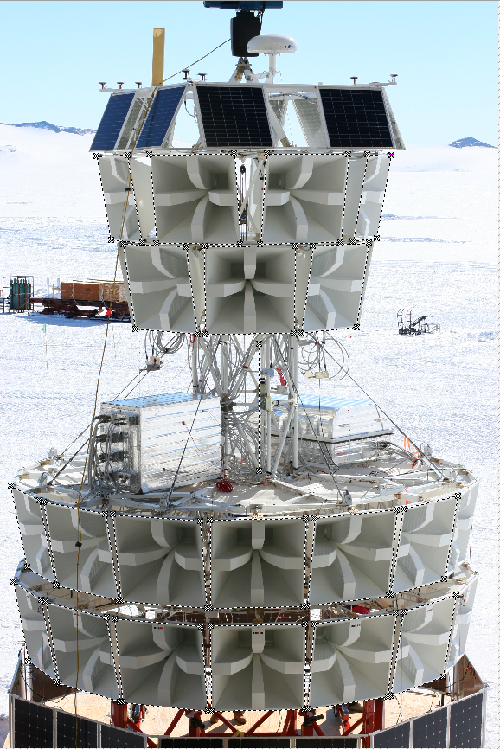
\includegraphics[height=0.5\textheight]{figures/KBelovANITA-III_photogrammetry_update-3}
		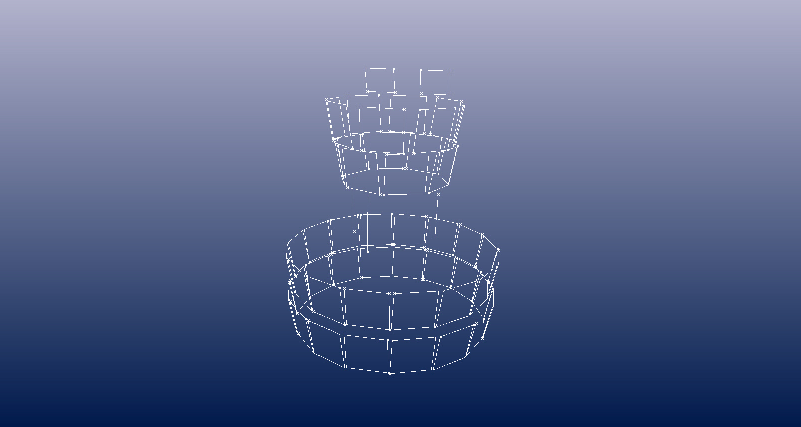
\includegraphics[width=\textwidth]{figures/KBelovANITA-III_photogrammetry_update-4}
		\caption{Top: Example photogrammetry image of the ANITA3 payload with markers drawn around the antenna face outlines.  Bottom: Subsequent wiremesh model of antenna positions derived from numerous combined images.  Thanks to Constantine for images.}
	\end{figure}
	
		
	\subsection{Calibration Pulse Timing Optimization}
		The electrical center-point of the antennas, though directly related to the physical position and orientation of the antenna, requires an additional calibration.  The phase center, or point at which the electromagnetic field couples to the antenna and begins propagating through the signal cables, is a function of frequency and incident wave direction, so the calibration must consider a large phase space.  The calibration measurements are done in-situo by a ground pulser at WAIS divide sending a pulse to the payload as it passes overhead.  This pulse can be used to determine  the relative phase center offsets between nearby antennas.  The positional error of the phase centers relates directly to the pointing error for events seen later in the flight.
		
		The two pulser locations discussed earlier provide two distinct timeframes during which to measure the phase centers of the antennas.  

\section{System Impulse Response}
		The signal observed by the digitizers is strongly effected by the band limiting filters and 
		
	\subsection{Effect of Signal Chain}
	
	\subsection{Convolution with Antenna Response}
		An important effect on the signal measured by the instrument is the angular response of the antennas.  First, there are a few considerations for determining what the optimal antenna response, the ratio of induced voltage on the 50-ohm output terminal of the antenna as a function of electric field on the front face, as a function of angle.  Firstly, it is important for the antennas to have some response outside of their specific 22.5 degree wide phi sector observations region in order to have baselines with measurable signal power (is this true?  It only is an effect if the source is exactly centered with the phi sector, but then you sort of know where it is because neither surrounding phi sector has any power...).  The antennas also need to have a high gain, aka a high directivity, in order to increase signal power as a function of noise power.  If we only used omni-directional antennas, the interferometry would have additional baselines (as additional antennas would observe any specific signal source), however each channel would have a reduced signal power with an identical noise power.  This also doesn't take into account the occlusion of signal by the gondola structure and discrete instrument packages residing ont the deck.  In addition, there exists no perfect antenna with a step function response, and as such we need to characterize the non-ideal antennas that fly on ANITA3.
		These antennas have several measurements that describe the complex response (antenna gain and group delay as a function of frequency) of the flight antennas.  One was done by the manufacturer, and several were done by us on the ground.  An additional calibration was possible in flight using the calibration pulsers and the random rotations of the gondola in respect to it.  The absolute measurements are most accurate in gain, as in the far field calibration measurements the absolute timing of the pulser was not synchronized.  However, both gain and phase have relative measurements as a function of angle.
		There are two measurements that go into the response of the antenna.  The first is the S11 (or VSWR) of the antenna.  This describes the amount of input power is actually transmitted radiatively out of the antenna as a function of frequency.  The second is the actual gain pattern, which describes \textit{where} that power is transmitted in space.  Both are invertible, and together can be used to determine the antenna height which is a relation between the electric field incident on the antenna and the voltage transmitted to the transmission line.
		Additionally there is a polarization component.  As we have interest in the polarization components (Stokes parameters) of the signal, the antennas are designed to be measure both vertical and horizontal polarizations independently.  Each polarization of the antenna has some non-trivial response in the opposite polarization however, especially in signals that have a combined vertical and horizontal component, which must be measured and factored out when for determining incident signal polarization.  For this, we have few measurements, and it may have to be done purely with in flight observations of known circularly polarized anthropogenic sources (such as satellites), thought that has an additional ionospheric component that would need to be measured.  In the end we may need to just extend error bars for this in leu of additional chamber measurements.
		
	\subsection{Effect of Uneven Time Sampling}
	The uneven sampling produced by the non-idealities of the LABRADOR sampling timebase requires the waveform to be evenly resampled before it can be properly compared to other waveforms in each event.  In addition, the timing offsets induced by the physical baseline delays between antennas as well as the internal asynchronous hold times are not quantized to the sample bins, and thus must be up-sampled to be properly correlated and averaged.  There are several methods that can be used to accomplish this, each with drawbacks and positives.

	

	
	
\section{Triggering Sanity Check}
		Before flight, a programmable delay line was used to input picosecond precision delayed impulses into channels within neighboring phi sectors to test for the true angular response of the payload.  Due to the opaque nature of firmware, it is important to discern the exact L0 coincidence regions in which a global trigger will be generated.
	\subsection{Angular Response Characteristics From Data}

\section{Non-uniform Channels and Outliers}
	There are several channels in the ANITA3 instrument that are non-uniform.  The first, and most obvious, is the channel in which the ALFA is digitized.  The desire to have a 97th low frequency drop down omni-azimuthal responce digitizing antenna required an additional channel, however there were none available.  To accommodate this, a modified filter was placed on channel 05TH that limited the nominal input signal to 800Mhz.  The low frequency (40-80MHz) antenna was then heterodyned with a 900Mhz local oscillator (LO) which produces a upsampled beat pattern at $f_(LO)-f_(ALFA)$ and $f_(LO)+f_(ALFA)$. This channel must be treated slightly differently than the rest in a few ways.  First, the signal must be digitally filtered to remove the ALFA component before it is correlated or averaged with similar antennas.  Secondly, in simulation the reduced bandwidth (and subsequent lower noise and signal power) must be taken into account.





%%%%%%%%%%%%% 4 %%%%%%%%%%%%%%%%%%%%%%%%%%%%%%%%%%%%%%%%%%%%%%%%%%%%%%%%%%%%%%%%%%%%%%%%%%%%%%%%%%%%%%%%%%%%%%%%%%%%%%%%
\chapter{Cosmic Ray Search with ANITA3 Flight Data}
%%%%%%%%%%%%%%%%%%%%%%%%%%%%%%%%%%%%%%%%%%%%%%%%%%%%%%%%%%%%%%%%%%%%%%%%%%%%%%%%%%%%%%%%%%%%%%%%%%%%%%%%%%%%%%%%%%%%%%%%
\section{ANITA3 Flight Overview}
	The data recorded by the ANITA3 flight instrument requires a significant analysis effort to extract a meaningful physics result.  In our case, we need to use the raw digital values read out for each channel to determine the analog electromagnetic environment surrounding the payload during brief moments the trigger system determined a physics event may be occurring.  From this, we can use an understanding of the physical geometry of the antennas mounted on the payload, including their orientation and electrical responses, to determine the cause of any incident wave patterns read out by the digitizers.  Once these wave patterns are identified and classified, they can be sorted into signal and background thermal or anthropogenic noise sources via a series of procedural cuts.  This section details the process and results of this analysis.
	
\section{Analysis Overview}
	The analysis for this flight was done with the premise that we are searching for "cosmic ray like" events.  As there are already published observations of cosmic rays from previous ANITA flights, I can reduce the workload of doing a full blind analysis with the consequence of excluding signals that do not fit into a measured and modeled EAS radiation pattern.  This still will allow us to search for two separate cosmogenic particles, cosmic rays and tau neutrino regeneration events.

	\subsection{In Flight Modifications}
		
	
\section{Blinding Procedure}

	\subsection{Philosophical Reasoning For Blinding}
	
	\subsection{Threshold for Unblinding Request}

	\subsection{Polarization Specific Blinding}

\section{Event Quality Cuts}

\section{Constant wave source filtering}
	Anthropogenic signals used for communications often take the form of high powered circularly polarized constant wave sources.  These signals are present in much of the data, and their effect on the trigger is twofold.  Firstly, they compress the tunnel diode by increasing the total power of the input signal, elevating the diode response out of the square-law range.  Second, they force an increase in the threshold voltage used on the comparator circuit used to trigger on the signals.  Despite these two effects, impulsive candidate signals can still be hidden superimposed on the CW source.  To remediate the effects of these signals on the pointing and post-flight analysis, we can apply a filter that only notches out a specific frequency band of the signal.
	\subsection{Bookkeeping and Filtering Decision Heuristic}
	\subsection{Fourier Domain Band Filtering}
			The easiest way to filter out CW signals is to set the magnitude of the complex Fourier phasors to zero in frequency bands that exceed some expected flat spectral slope.  Though this is computationally quite easy, this process is not causal, and will harm the integrity of the resultant signal.
		\subsection{Sine wave subtraction}
			A more computationally intensive method for eliminating CW sources is a method where a sine wave is fit to the measured waveform and iteratively subtracted.  This process preserves the causality of the signal, as it is done purely in the time domain, and also decreases the width of the band that will be filtered, preserving more total signal power if it exists in the measurement.  The drawback of this method is that it requires a fit, which is takes time and is prone to failure.


\section{De-dispersion}
	The antenna, filters, cables, and amplifiers are responsible for introducing a frequency dependent gain and group delay to the observed signals.  These elements act to disperse the power in the signal across tens of nanoseconds from what was emitted from the relativistic shower at the critical angle as a highly impulsive, picosecond length essential delta-function like electromagnetic field transient.  The impulse response, or complex phasor representation of this dispersive effect, was measured for the signal chain immediately preceding the flight for each of the 96 channels, and for all 48 antennas in a controlled manner in Palestine the summer beforehand.  These two effects are then combined and used to determine a whole system impulse response that relates the measured ADC values at the LABRADOR digitizer to an electric field incident at the payload.  By reversing the dispersive process, via Weiner deconvolution (described below), we can both increase the instantaneous power of a signal and compare it directly to the electric field radiation output of high energy particle shower simulations such as COREAS or ZHAires.
	\subsection{Generation of transfer function}
		The transfer function of the system was painstakingly developed and utilized a variety of both time domain and Fourier transformed frequency domain manipulations.  These each introduce their own errors, as many of them require assumptions about the incoming signal.  I'll detail the full process of generating the transfer function in an appendix.
	\subsection{Signal to noise ratio of impulse response}
		Any band limited deconvolution process requires a knowledge of the signal to noise ratio of the transfer function as a function of frequency (SNR(f)).  Since the transfer function merely relays the amplitude and phase differences between an input and output signal (represented in either a complex phasor or a time domain waveform), one must also have an understanding of the total power contained within the input and output signals.  If, for example, both the input and output signal contained very little power out of a specified band pass, it could be wrongly assumed from a transfer function that the signal chain was able to pass frequencies that are out of the band pass.
		The "signal" and "noise" of this must therefore be defined, as the spectral power has multiple sources.  The principle   
	\subsection{Weiner Deconvolution}
		The impulse response used to deconvolve waveforms is 

\section{Polarization cuts}

\section{Event Reconstruction}
	The major tool used in the ANITA analysis is a radio astronomy technique that uses the physical separation between the antennas and the correlations of waveforms from these antennas to generate a map of likely pointing directions.  ANITA has three vertical tiers of antennas, each separated from each other, and at least three co-pointing phi sectors that are expected to observe events from any angle.  Using the combined baseline offsets from these antennas, it is possible to overlay 9 different interferometric maps to create a pointing map.  By finding the peak of this map, a vector pointing away from the payload can be traced to the ice, where a map of the vertical height of the continent can be used to create a map of events on the ground.
	\subsection{Radio Interferometric Pointing}
	\subsection{Ray Tracing to Continent (with index of refraction)}
	\subsection{Log-Likelyhood Two Dimensional Gaussian Pointing Error}
	\subsection{Immediate Pointing Cuts}


\section{Known object categorization}
	Many bases on the Antarctic continent are already cataloged by the various national programs that operate them.  Using these known bases we can eliminate events that interferometrically point to objects of expected anthropogenic noise.  There also likely exist bases that are, for whatever reason, not included in our catalog.  We also use a list of "pseudo-bases" generated from clustered event lists from previous ANITA flights to eliminate possible anthropogenic interference.  The resulting effect these excluded regions have on the flight can be determined by its flight path and a log-likelyhood method for generating pointing error elipses around the bases.  I'll put a plot of that here.
	\subsection{Sun and Its Reflection, Thermal Noise Effect}
	\subsection{Satellites, Bases, and other Anthropogenic Sources}

\section{Thermal Noise Separation Results}
	\subsection{Cut Efficiency}
	\subsection{Cut Quality}


\section{Base and non-base clustering}
	\subsection{Clustering Purity and Efficiency}


	
	

%%%%%%%%%% 5 %%%%%%%%%%%%%%%%
\chapter{Simulation of Air Shower Event in Time Domain and Expected Event Rate from Analysis Techniques}
%%%%%%%%%%%%%%%%%%%%%%%%%%
\section{Air Shower Simulation Overview}
	The series of analysis procedures used to categorize events into signal and noise boxes
	\subsection{ZHAires Shower Modeling}
		Radio emission from cosmic ray air showers is accomplished by using the ZHS extension to the AIRshower Extended Simulations (AIRES) package.\cite{AlvarezMuñiz2012325}  This framework, developed by Jaime Alvarez-Muniz, Washington Rodrigues de Carvalho Jr. and Enrique Zas, generates a time varient electric field for a configurable incident particle at some instrumentation point in the atmosphere.  Recent work with ANITA in mind has further extended the simulation to accurately depict reflections off the ice sheet.
		
		Simulations provide an important method to determine the overall sensitivity of the ANITA instrument to air shower events as a function of incident angle and energy and payload location.  Due to the coherent beamed characteristic of air shower radio emmission, specifically a peak at the critical Cherenkov angle from the shower axis, ANITA is only sensitive to a small fraction of showers.
		
		The spectral content of EAS radiation falls off sharply as a function of offset from the critical Cherenkov angle.  Without being within a few degrees of the peak coherence angle, low frequency radiation, below the band of the ANITA instrument, dominates the spectrum.  This can be seen in Figure figure.  
		
\section{IceMC: ANITA Monte Carlo Simulation Package}
	
\section{Instrumented Volume Estimate}
			
			
%%%%%%%%%%%%% 6 %%%%%%%%%%%%%	
\chapter{Results of Analysis and Limits}
%%%%%%%%%%%%%%%%%%%%%%%%%%%%%
\section{Cut Event Results}

\section{Event Pointing Results}
	\subsection{Additional Pseudo-Base Candidates}


\section{Cosmic Ray Candidates}

\section{Cosmic Ray Flux Estimate}

\section{$\nu$-$\tau$ Candidates}

\section{$\nu$-$\tau$ Flux Estimates}

			
%%%%%%%%%%%%%%% 7 %%%%%%%%%%%%%%%
\chapter{Quick and Dirty Reanalysis of ANITA2 Data Using Corrected dTs}
%%%%%%%%%%%%%%%%%%%%%%%%%%%%%%%%%%
\section{Issues with previous analysis of ANITA2 flight data}
	The ANITA2 flight analysis contains a time base calibration with an unexpectedly and overlooked wide dT variance.  This has the effect of limiting the response from high frequency signals, an effect not taken into account when the analysis was completed.

\section{"Golden Event" Cosmic Ray Time Bin Correction}

\section{Effects on ANITA2 Flux Limits}
			
			
%%%%%%%%%%%%%% 8 %%%%%%%%%%%%%%%%%%%%		
\chapter{Conclusion and Discussion}
%%%%%%%%%%%%%%%%%%%%%%%%%%%%%%%%%%%%%
	UHECRs continue to present a variety of fundamental issues for the astrophysics community.  These include 
\section{Limits set by other experiments}

\section{Future Prospects for UHECR Detection}


	
			
			
			
			
%%%%%%%%%%%%%%%%%%%%%%%%%%%		
\chapter{Appendix A}
%%%%%%%%%%%%%%%%%%%%%%%%%%%
\section{Overview}
	This appendix deals primarily with the detection of Anti-Quark Nuggets, an exotic dark matter candidate particle, using the ANITA power monitor subsystem.
	
	
	\subsection{Sensitivity}
		The sensitivity of the power monitor is driven mainly by the digital averaging of the digitized signal done in firmware.
	\subsection{Improvement over ANITA2}
		The ANITA2 instrument did not have any digital averaging, and relied on a mal-designed analog low pass filter which significantly reduced both the sensitivity of the power monitor and the observed time.  Since the readout was only done at 10Hz, and the integration window was on the order of microseconds, a majority of time was left un-sampled.  This was improved in the ANITA3 flight to include a high factor of digital averaging.  This modification is discussed in detail in Appendix A.
	
	
	

